%%%%%%%%%%%%%%%%%%%%%%%%%%%%%%%%%%%%%%%%%%%%%%%%%%%%%%%%%%%%%%%%%%%%%%
%%  disstemplate.tex, to be compiled with latex.		     %
%%  08 April 2002	Version 4				     %
%%%%%%%%%%%%%%%%%%%%%%%%%%%%%%%%%%%%%%%%%%%%%%%%%%%%%%%%%%%%%%%%%%%%%%
%%								     %
%%  Writing a Doctoral Dissertation with LaTeX at		     %
%%	the University of Texas at Austin			     %
\documentclass[12pt]{report}	% The documentclass must be ``report''.

\usepackage{utdiss2}  		% Dissertation package style file.

\usepackage{natbib}
%%%%%%%%%%%%%%%%%%%%%%%%%%%%%%%%%%%%%%%%%%%%%%%%%%%%%%%%%%%%%%%%%%%%%%
% Optional packages used for this sample dissertation. If you don't  %
% need a capability in your dissertation, feel free to comment out   %
% the package usage command.					     %
%%%%%%%%%%%%%%%%%%%%%%%%%%%%%%%%%%%%%%%%%%%%%%%%%%%%%%%%%%%%%%%%%%%%%%

\usepackage{amsmath,amsthm,amsfonts,amscd} 
				% Some packages to write mathematics.
\usepackage{eucal} 	 	% Euler fonts
\usepackage{verbatim}      	% Allows quoting source with commands.
\usepackage{makeidx}       	% Package to make an index.
%\usepackage{epsfig}         	% Allows inclusion of eps files.
%\usepackage{epsfig}         	% Allows inclusion of eps files.
%\usepackage{cyrchar}
%\usepackage{citesort}         	% 
\usepackage{url}		% Allows good typesetting of web URLs.
\usepackage{draftcopy}	
\usepackage{graphicx}
\usepackage{amsthm}
%\usepackage{amssymb}
%\usepackage{epstopdf}
%\DeclareGraphicsRule{.tif}{png}{.png}{`convert #1 `dirname #1`/`basename #1 .tif`.png}

\usepackage[utf8]{inputenc}
\usepackage{CharisSIL}
\usepackage{booktabs}
\usepackage{topcapt}
\usepackage{subcaption}
%\usepackage{wrapfig}



\usepackage{leipzig}
\usepackage{gb4e}



\author{sally ransom}  	% Required

\address{305 E. 23rd Street STOP B5100\\ Austin, Texas 78712}  % Required

\title{becoming lyrics: how word prosody and musical meter negotiate the rhythmic terms of prominence}
                                                    % Required


%
% NOTE: Maximum three supervisors. Minimum one supervisor.
% NOTE: The Office of Graduate Studies will accept only two supervisors!
% 
%
\supervisor
	[Scott Myers]
	{Katrin Erk}

%%%%%%%%%%%%%%%%%%%%%%%%%%%%%%%%%%%%%%%%%%%%%

%%%%%%%%%%%%%%%%%%%%%%%%%%%%%%%%%%%%%%%%%%%%%%%%%%%%%%%%%%%%%%%%%%%%%%

\previousdegrees{B.A., Linguistics}
     % The abbreviated form of your previous degree(s).
     % E.g., \previousdegrees{B.S., MBA}.
     %
     % The default value is `B.S., M.S.'

%\graduationmonth{...}      
     % Graduation month, either May, August, or December, in the form
     % as `\graduationmonth{May}'. Do not abbreviate.
     %
     % The default value (either May, August, or December) is guessed
     % according to the time of running LaTeX.

%\graduationyear{...}   
     % Graduation year, in the form as `\graduationyear{2001}'.
     % Use a 4 digit (not a 2 digit) number.
     %
     % The default value is guessed according to the time of 
     % running LaTeX.

%\typist{...}       
     % The name(s) of typist(s), put `the author' if you do it yourself.
     % E.g., `\typist{Maryann Hersey and the author}'.
     %
     % The default value is `the author'.


%%%%%%%%%%%%%%%%%%%%%%%%%%%%%%%%%%%%%%%%%%%%%%%%%%%%%%%%%%%%%%%%%%%%%%
% Commands for master's theses and reports.			     %
%%%%%%%%%%%%%%%%%%%%%%%%%%%%%%%%%%%%%%%%%%%%%%%%%%%%%%%%%%%%%%%%%%%%%%
%
% If the degree you're seeking is NOT Doctor of Philosophy, uncomment
% (remove the % in front of) the following two command lines (the ones
% that have the \ as their second character).
%
\degree{MASTER OF ARTS}
\degreeabbr{M.A.}

% Uncomment the line below that corresponds to the type of master's
% document you are writing.
%
%\masterreport
\masterthesis


%%%%%%%%%%%%%%%%%%%%%%%%%%%%%%%%%%%%%%%%%%%%%%%%%%%%%%%%%%%%%%%%%%%%%%
% Some optional commands to change the document's defaults.	     %
%%%%%%%%%%%%%%%%%%%%%%%%%%%%%%%%%%%%%%%%%%%%%%%%%%%%%%%%%%%%%%%%%%%%%%
%
%\singlespacing
%\oneandonehalfspacing

%\singlespacequote
\oneandonehalfspacequote

\topmargin 0.125in	% Adjust this value if the PostScript file output
			% of your dissertation has incorrect top and 
			% bottom margins. Print a copy of at least one
			% full page of your dissertation (not the first
			% page of a chapter) and measure the top and
			% bottom margins with a ruler. You must have
			% a top margin of 1.5" and a bottom margin of
			% at least 1.25". The page numbers must be at
			% least 1.00" from the bottom of the page.
			% If the margins are not correct, adjust this
			% value accordingly and re-compile and print again.
			%
			% The default value is 0.125"

		% If you want to adjust other margins, they are in the
		% utdiss2-nn.sty file near the top. If you are using
		% the shell script Makediss on a Unix/Linux system, make
		% your changes in the utdiss2-nn.sty file instead of
		% utdiss2.sty because Makediss will overwrite any changes
		% made to utdiss2.sty.

%%%%%%%%%%%%%%%%%%%%%%%%%%%%%%%%%%%%%%%%%%%%%%%%%%%%%%%%%%%%%%%%%%%%%%
% Some optional commands to be tested.				     %
%%%%%%%%%%%%%%%%%%%%%%%%%%%%%%%%%%%%%%%%%%%%%%%%%%%%%%%%%%%%%%%%%%%%%%

% If there are 10 or more sections, 10 or more subsections for a section,
% etc., you need to make an adjustment to the Table of Contents with the
% command \longtocentry.
%
%\longtocentry 



%%%%%%%%%%%%%%%%%%%%%%%%%%%%%%%%%%%%%%%%%%%%%%%%%%%%%%%%%%%%%%%%%%%%%%
%	Some math support.					     %
%%%%%%%%%%%%%%%%%%%%%%%%%%%%%%%%%%%%%%%%%%%%%%%%%%%%%%%%%%%%%%%%%%%%%%
%
%	Theorem environments (these need the amsthm package)
%
 \theoremstyle{plain} %% This is the default

\newtheorem{thm}{Theorem}[section]
\newtheorem{cor}[thm]{Corollary}
\newtheorem{lem}[thm]{Lemma}
\newtheorem{prop}[thm]{Proposition}
\newtheorem{ax}{Axiom}

\theoremstyle{definition}
\newtheorem{defn}{Definition}[section]

\theoremstyle{remark}
\newtheorem{rem}{Remark}[section]
\newtheorem*{notation}{Notation}

\numberwithin{equation}{section}


%%%%%%%%%%%%%%%%%%%%%%%%%%%%%%%%%%%%%%%%%%%%%%%%%%%%%%%%%%%%%%%%%%%%%%
%	Macros.							     %
%%%%%%%%%%%%%%%%%%%%%%%%%%%%%%%%%%%%%%%%%%%%%%%%%%%%%%%%%%%%%%%%%%%%%%
%
%	Here some macros that are needed in this document:


\newcommand{\latexe}{{\LaTeX\kern.125em2%
                      \lower.5ex\hbox{$\varepsilon$}}}

\newcommand{\amslatex}{\AmS-\LaTeX{}}

\chardef\bslash=`\\	% \bslash makes a backslash (in tt fonts)
			%	p. 424, TeXbook

\newcommand{\cn}[1]{\texttt{\bslash #1}}

\makeatletter		% Starts section where @ is considered a letter
			% and thus may be used in commands.
\def\square{\RIfM@\bgroup\else$\bgroup\aftergroup$\fi
  \vcenter{\hrule\hbox{\vrule\@height.6em\kern.6em\vrule}%
                                              \hrule}\egroup}
\makeatother		% Ends sections where @ is considered a letter.
			% Now @ cannot be used in commands.

\makeindex    % Make the index

%%%%%%%%%%%%%%%%%%%%%%%%%%%%%%%%%%%%%%%%%%%%%%%%%%%%%%%%%%%%%%%%%%%%%%
%		The document starts here.			     %
%%%%%%%%%%%%%%%%%%%%%%%%%%%%%%%%%%%%%%%%%%%%%%%%%%%%%%%%%%%%%%%%%%%%%%

\begin{document}

\copyrightpage          % Produces the copyright page.


%
% NOTE: In a doctoral dissertation, the Committee Certification page
%		(with signatures) is BEFORE the Title page.
%	In a masters thesis or report, the Signature page
%		(with signatures) is AFTER the Title page.
%
%	If you are writing a masters thesis or report, you MUST REVERSE
%	the order of the \commcertpage and \titlepage commands below.

\titlepage              % Produces the title page.
%
\commcertpage           % Produces the Committee Certification
			%   of Approved Version page (doctoral)
			%   or Signature page (masters).
			%		





%%%%%%%%%%%%%%%%%%%%%%%%%%%%%%%%%%%%%%%%%%%%%%%%%%%%%%%%%%%%%%%%%%%%%%
% Dedication and/or epigraph are optional, but must occur here.      %
%%%%%%%%%%%%%%%%%%%%%%%%%%%%%%%%%%%%%%%%%%%%%%%%%%%%%%%%%%%%%%%%%%%%%%
%
\begin{dedication}
\index{Epigraph@\emph{Epigraph}}%

\begin{quotation}
{\scriptsize I think that when linguists discuss and dispute sound length and stress among themselves they would definitely benefit from inviting ethno-musicologists to join them. They could discuss the issues together, and not only based on written records but also sung records. \\ 
That what is written is fiction. Only that what is sung is truth. \\
\cite{tormisProblemsThatRegilaul2007} }



\end{quotation}

\end{dedication}


%\begin{acknowledgments}		% Optional
%\index{Acknowledgments@\emph{Acknowledgments}}%
%I wish to thank the multitudes of people who helped me. Time would
%fail me to tell of \ldots
%\end{acknowledgments}


% The abstract is required. Note the use of ``utabstract'' instead of
% ``abstract''! This was necessary to fix a page numbering problem.
% The abstract heading is generated automatically.
% Do NOT use \begin{abstract} ... \end{abstract}.
%
\utabstract
\index{Abstract}%
\indent
%
%
%This paper analyses the acoustic realizations of sung vowels in Estonian {\it regilaul} lyrical folksong performances to examine the effects of musical metrical structure on the word-prosodic level of the language. Estonian is of particular interest as it has a fixed, predictable word stress pattern and three  syllable weights. In light of these features, I compare documented acoustic correlates of both stress and syllable weight, and the effects of them falling ``on" or ``off" the beat within the trochaic tetrametric pattern of {\it regilaul}. Vowel space and duration of syllable nuclei is compared in stressed and unstressed syllables falling on and off the beat in song, and all three quantities in word-prosodic stressed position examined on and off the beat in the song. 


 \tableofcontents   % Table of Contents will be automatically
                   % generated and placed here.

\listoftables      % List of Tables and List of Figures will be placed
\listoffigures     % here, if applicable.



%%%%%%%%%%%%%%%%%%%%%%%%%%%%%%%%%%%%%%%%%%%%%%%%%%%%%%%%%%%%%%%%%%%%%%
% Actual text starts here.					     %
%%%%%%%%%%%%%%%%%%%%%%%%%%%%%%%%%%%%%%%%%%%%%%%%%%%%%%%%%%%%%%%%%%%%%%
%


%
\chapter{Introduction}
\index{Introduction@\emph{Introduction}}%is

\section{On words becoming lyrics}
to join song and become lyrics, meaningful linguistic utterances are modified to fit the strict temporal structure of music while preserving intelligibility sufficient for semantic interpretation of the whole. 

Estonian is famous for its ternary quantity distinction: both vowels and consonants have three distinct lengths or degrees. As can be seen in the examples in \ref{ternary}, the length of a given segment can indicate lexical contrasts as in sada vs saada (`hundred' vs `send') (root minimal pairs) and also indicate case: the difference between `receive' and `send' is in the quantity of the first syllable' or directional case marking `of' versus `'into' the cupboard. 



 \begin{table}[htb]
\centering
\begin{tabular}{lcc}
\hline

Q1 &		 sada 		& 	kabi  \\  
	&	 {\it `hundred'} 	&	 {\it`hoof' }\\
\hline
Q2 &		saada 		&	kapi \\
	&	 {\it`send' }		&	{\it`of the cupboard' }		\\
\hline
Q3 &		saada 	&	 kappi 	\\
	&	{\it`recieve' }	&	{\it`into the cupboard' }	\\
\hline
\end{tabular}
\label{qexamps}
\caption{ternary syllable weight contrast}
\end{table}

. If the performer wishes the audience to perceive meaningful lyrical content, these contrasts must be crystallized at some level of salience in the acoustic signal. 
%
%This project takes folksong performance as an opportunity to examine the interface of language and music. In particular, I investigate the acoustic manifestations of the word-prosodic features attested in spoken Estonian when they are sung in a temporally restricted domain such as music. 


here I define metrical as the mapping of the pattern on a frame formed of equal time intervals: such patterns have been demonstrated to be more easily replicated by humans, something that is necessary for both the synchronization of musicians performing together and for the transmission of an oral tradition of songs \citep{essensPovel1985}. 

%
%\subsection{song lyrics as the music-language interface}
%
%In order 


\subsection{Metrical Principles of Estonian folksong}


In music, the smallest prosodic constituent is an individual note event whose relationship to the other notes in the song are indicated by the time signature, i.e., 3/4 or 4/4. The denominator corresponds to the number of divisions of a ``whole'' note, while the numerator refers to the number of ``beats'' in a single measure. So the prosodic heirarchy in music begins at the note level, then to each measure as constituent, larger phrases and motifs, and eventually the highest level which is the entire song. 

In Eesti, attested segments are organized into syllables, which in turn combine in strong-weak relationships to form prosodic feet, which make up the words of phrases and so on. 
both regilaul and Eesti have heirarchichal metrical systems by which long and short, stressed and unstressed constituents are arranged. 
 In a regilaul verse line, each syllable corresponds to an eighth note in the measure, with every odd positioned syllable-note coinciding with the ``beat'' onset in a typical 4/4 measure. Falling on the beat in music generally coincides with increased prominence compared to notes occurring ``off'' the beat. This is acoustically manifested in increased duration of notes on the beat compared to nominally isochronous notes in other positions. That is, in a measure containing eight eighth notes, the absolute durations of the four eighth notes corresponding to the beat will be longer than the absolute durations of the four eighth notes in even positions, while maintaining the perception of the nominal isochrony. 


How do the word-prosodic requirements negotiate with the imposed prosodic hierarchy of music? The rhythmic organization of song is said to integrate the prosodic structure of the language with musical rhythmic principles \citep{palmer1992}. However, earlier studies of {\it regilaul} explored temporal aspects of the songs and found that duration characteristics that would usually indicate important semantic differences lost their distinctions partially or entirely. Assuming that the intention of the singer is for the lyrics to be understood, I hypothesize that if some durational correlates of contrasting word-prosodic constituents are made less distinct in the process of compromising with the song that some other acoustic correlate of the relevant contrast at the word-prosodic level will be present, if not enhanced.  


\begin{figure}[htbp]
\begin{center}
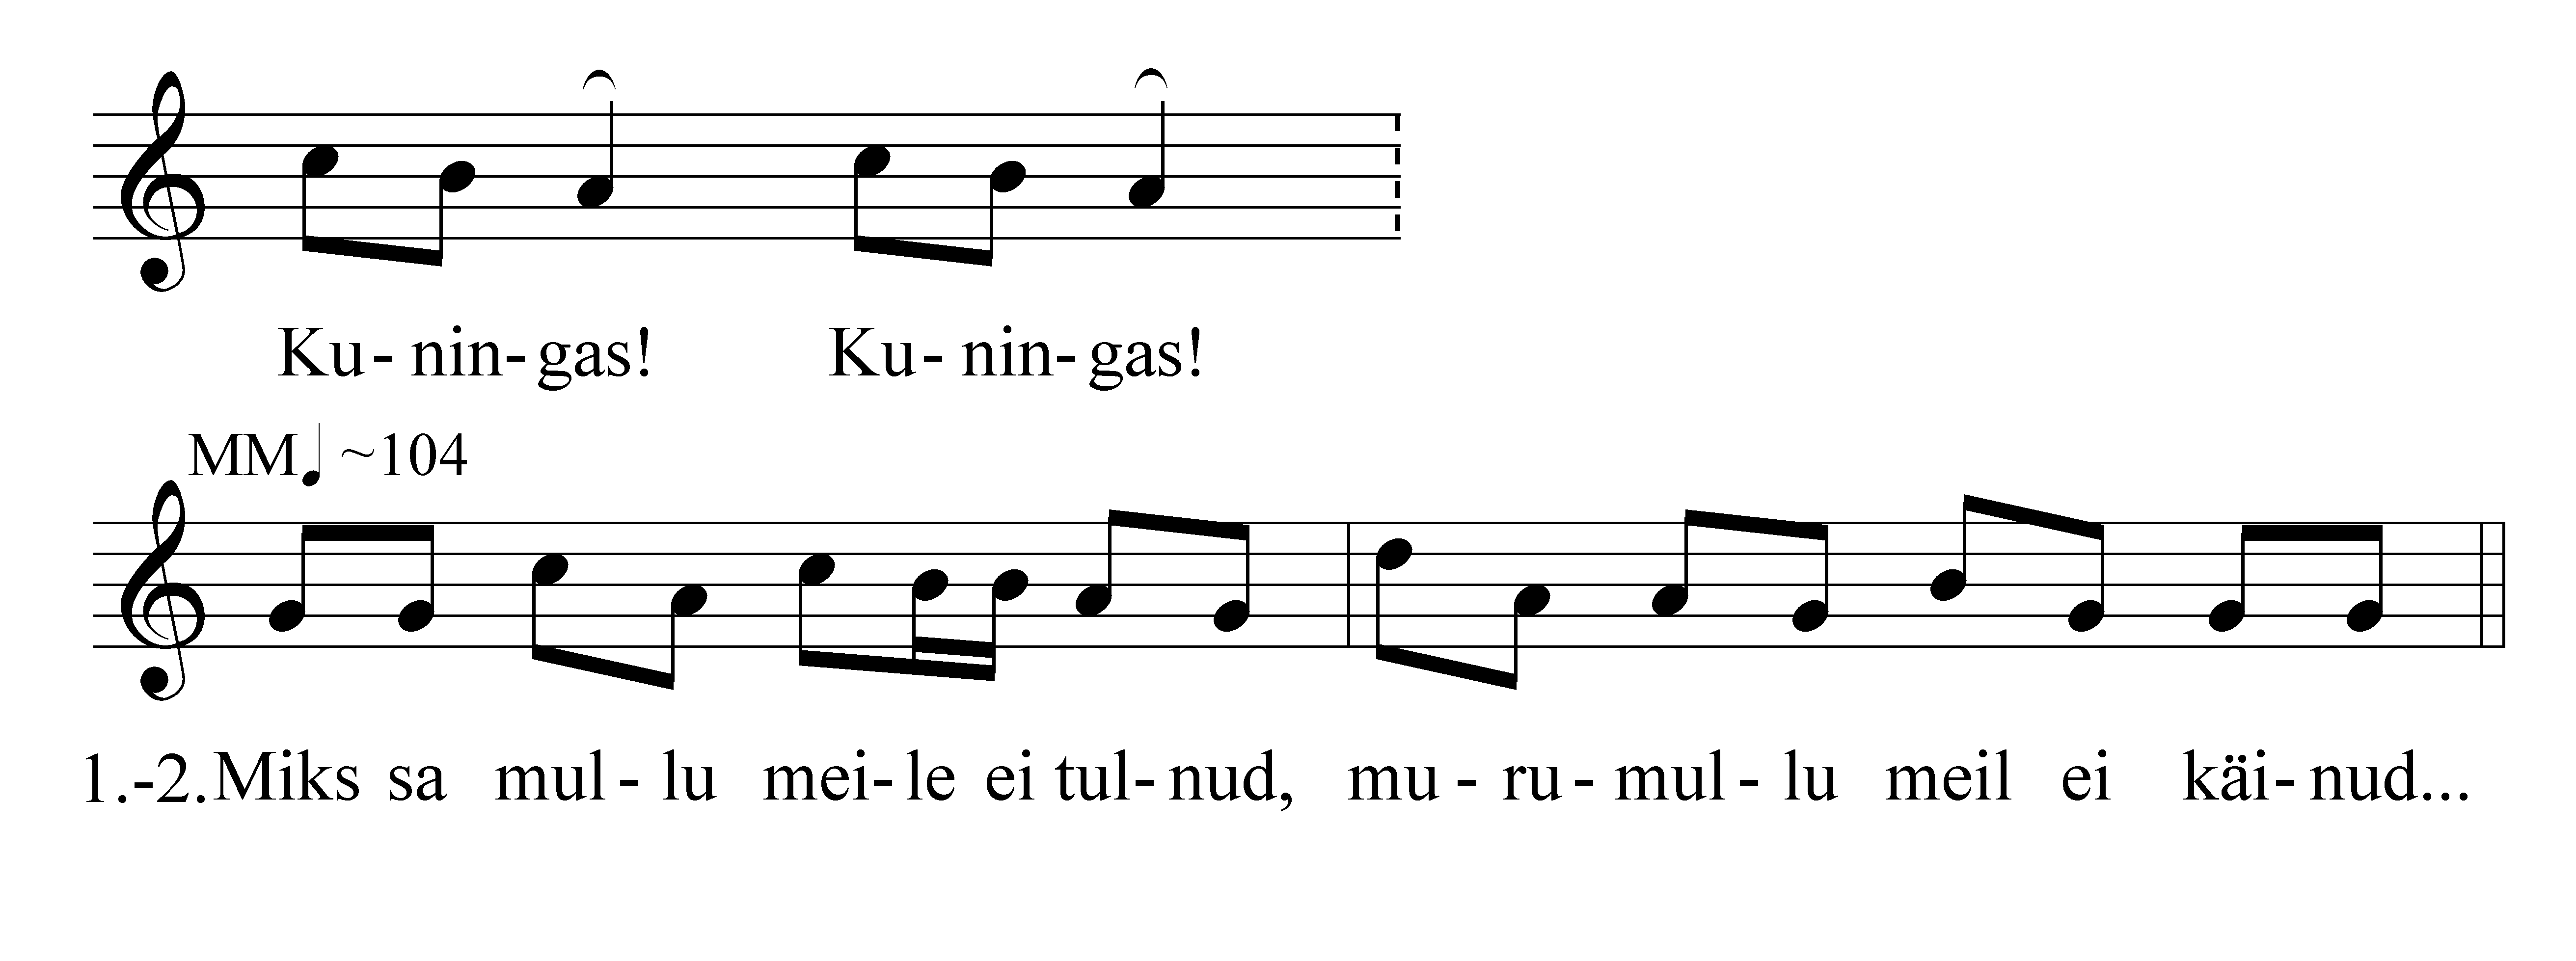
\includegraphics[width=300pt]{figures/094.png}
\caption{music notation of ``The King Game" as performed by Liisa Kümmel}
\label{The King Game}
\end{center}
\end{figure}

%\section{The Runic Song Tradition} 
%
%
%A given {\it regilaul} verse line contains eight beats, generally evenly divided into a single measure so that each of the eight syllables corresponds with one eighth note. The ictus position of a song's line is thus determinable by counting every other beat as ictus, starting with the first.
%
%The first song festival in Estonia held in \cite{ruutelTRADITIONALMUSICESTONIA2004}. 
%
%
%One runic invariant is that the tonal center is placed on ``the both syntactically stable 
%
%
%dominating pitch value of the most stable syntactical positions of a given melody's typological group
%
%
%the syllable-note is the basic unit of the melody-line. Thus syllables take up the space of the note in their position of the melody as prescribed. 

%Estonian, Finnish, Karelian, Ingrian runic songs
%
%whether it be Finnish, Estonian, Karelian, Votic, Ingrian and to same extent even Livonian an Veps)
%
%
the singable song \cite{tormis1985}
%
%
% ancient epic tale shared by many members of the Finno-Ugric language family
% 

 
 
 \cite{tormis2007}






 
\section{Previous Studies with regilaul}



The intuitions of ethnomusicologists who study the runosong tradition is that the burden of upholding the temporal structure of the song is the result of symbiosis between the musical rhythm and the natural prosodic features of the lyrical text \citep{ross1990, tampere1934}, inspiring over a decade of research at the interface of metrical phonetics and computational musicology. 
%
% 
%Melodic accents coincide with the stressed syllables, the pitch resolves as the phrase resolves. Said to be a musical abstraction of the natural prosodic intonation of the 8 syllable (spoken) runoverse \cite{ruutelResultsComputerizedComparative1999}.



\begin{figure}[htb]
\begin{center}
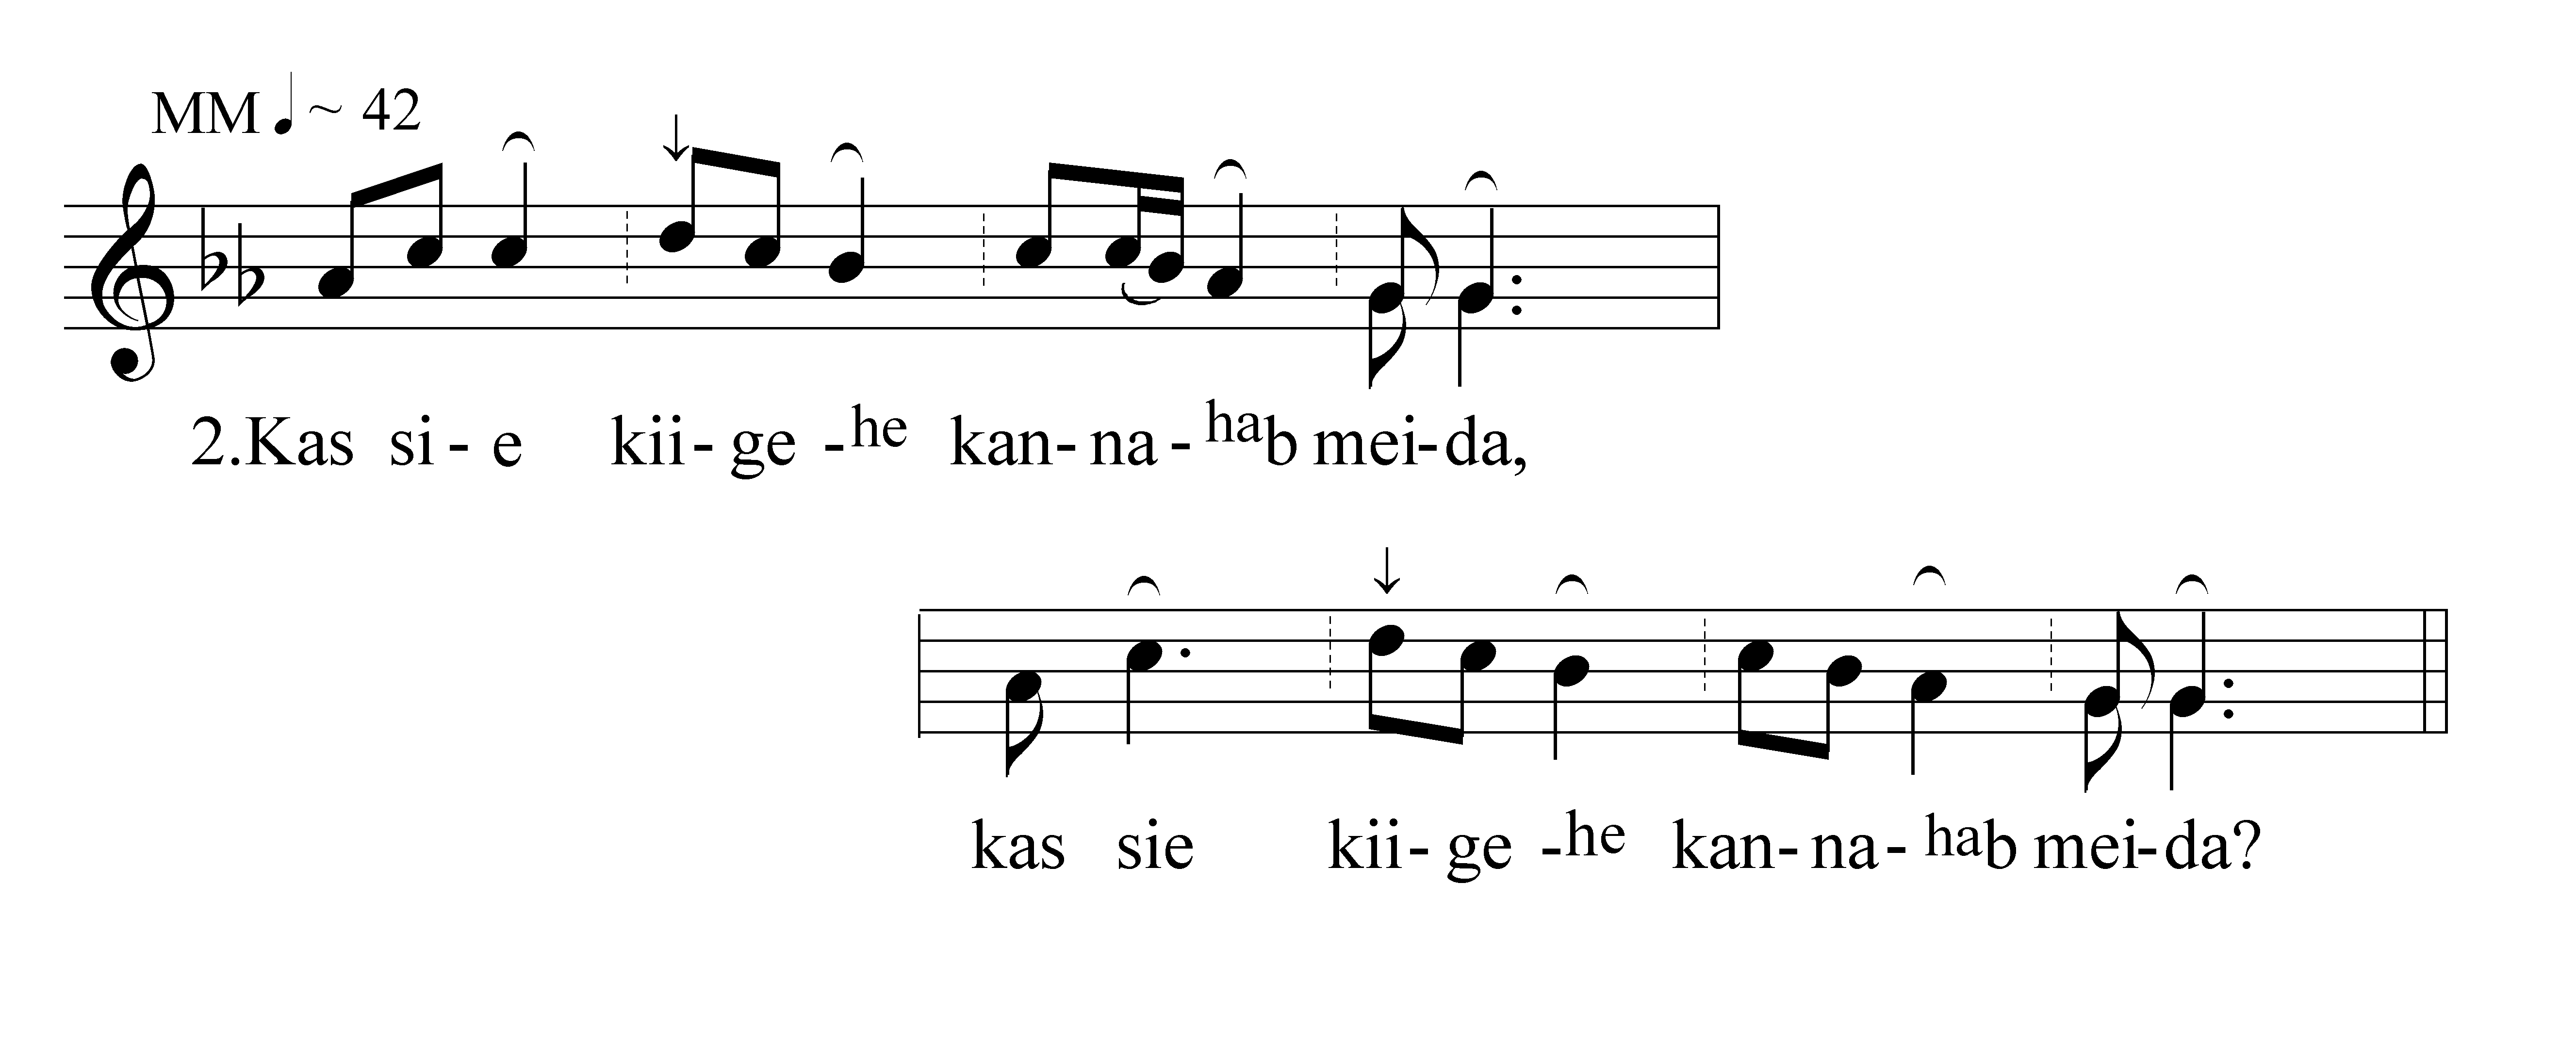
\includegraphics[width=300pt]{figures/022.png}
\caption{`Kiik tahab kindaid' \cite{}}
\label{022swing}
\end{center}
\end{figure}

Swinging songs are characterized by a swinging rhythm with alternating long and short notes, differing from the main body of {\it regilaul}'s iconic isochrony. 
Jaan Ross, a musicologist and native speaker of Estonian analyzed a 1936 recording of the swing song `Kiik tahab kindaid' \ref{022swing}, publishing results on syllable-note duration \cite{ross1989} and later the vowel quality of odd-numbered syllables \citep{ross90}. In the study on syllable-note durations, 

In the second, Ross measured formant frequencies f1 and f2, finding a reduced vowel space in song compared to measurements in spoken Estonian. However, upon examination of the song, it is clear that all the vowel space measurements are from syllable-notes in non-initial positions of Estonian words: that is, the sample of vowels taken from  the song were all unstressed, and compared to a mixed sample of spoken Estonian. Thus, the conclusion needs to be evaluated again with comparable samples. 

%
In 1992, Ilse Lehiste asked "Whether there is a correlation between poetic metre and the prosodic structure of a language.\citep{lehiste1992} by means of measuring the acoustic-phonetic realizations of so-called trochaic metrical poetic patterns across several languages including Estonian and Finnish. While these languages share in the more general Balto-Finnic tradition of {\it runosong} utlizing what is called the {\it Kalevala} meter, there were significant differences in the phonetic realizations of trochees in each language. 


In 1994, their collaboration begins. Ross and Lehiste published several papers examining the temporal dimensions of Estonian word prosody and metrical prominence in {\it regilaul} folksongs. In \citep{rossLehiste1994}, they conclude that duration differences ordinarily present at the word level (stressed-unstressed) are {\it ``lost"} to the temporal restrictions of the song. In another paper, syllable-notes are again measured, this time examining the role of syllabic quantity in the song. They likewise conclude that the duration of syllable-notes in {\it regilaul} match more closely with the metrical structure of the songs, that is, the durations of syllable-notes are best predicted by their beat position in the song: on the beat, syllables are longer, off the beat shorter. They extend this finding to conclude that the song "dominates" the metrical status of the words, claiming that the intelligibility of lyrics is enhanced more strongly by ``top-down" processes (i.e., semantic context). 

\citep{rossLehiste1996}. \\

%to paraphrase: Semantically relevant oppositions of word initial short-long and long-short disyllabic units in speech are not kept completely intact in folk songs. Short-long disyllables are treated in a different manner by the performer, depending on whether their initial syllable occurs at a rise or at a fall in a foot
\citep{rossLehiste1998} Analyzed and concluded that the {\it regilaul} lyrics are the result of an interaction between word and song prosodic hierarchies. This conclusion relied critically on measuring the durations of syllable-notes, where they found being on or off the beat was the better predictor for duration. \\


Finally, in %\citep{book_jril_2001} summarize their body of work until that point and extend their findings with fine-grained acoustic phonetic measurements of segment durations within syllable-notes. 

\section{The present study}

I do not dispute the findings that syllable-notes are best predicted by their position in the song. Instead, I argue that instead of an hierarchical interaction between language and music, what occurs is more akin to entrainment. Specifically, bidirectional entrainment of two oscillators. 

The syllable-notes, fit into the temporal structure of the music, still have possible acoustic-phonetic dimensions by which to indicate word boundaries (stressed-unstressed) and semantically-relevant quantity contrasts.  The durational differences of stress and quantity in spoken Estonian could be indicated either at another level of the prosodic hierarchy, i.e.,  the segment, or by enhancing another acoustic cue for prominence: i.e.,  vowel space dispersion. 


An EEG study of native Estonian speakers uncovered a perceptual asymmetry: shortening of constituents did not inducing MNN, but lengthening does \citep{eestiMNNasymmetry}. This suggests that stressed syllables, long in spoken Estonian, could be realized as shorter in a song without sounding ``off," but that lengthening of shorter elements would be less preferable. So long as syllable-notes maintain the relative durations in the song (i.e., heavy syllables are still longer than light ones), the metrical pattern of the musical phrase can be met. 

\subsection{Hypotheses}
Null hypothesis: on or off-beat position is best predictor for vowel duration of syllables in all categories: stressed, unstressed, short, long, and overlong. This would mean that the syllable nucleus is proportional to the total syllable duration, and that the duration contrast is indeed ``lost." 

H_{1}: duration contrasts for syllable quantity will be evident in the vowel duration, with vowel duration {\it decreasing} as syllable weight increases. Given the findings of \citep{rossLehiste2001}, isochronous syllable-notes would result in heavier syllables having shorter nuclei to accomodate for the coda and complex codas that distinguish the syllable weights from each other. 

H_{2}: stress/unstress contrasts will be evident in the nucleus in terms of hypo and hyper articulation. For this I measure both nucleus duration and vowel space dispersion. 

%\cite{rossStudyTimingEstonian1989,rossLostProsodicOppositions1994,rossTradeoffQuantityStress1996,sargDoesMelodicAccent2006, sargMelodicAccentEstonian2007,orasMusicalManifestationsTextual2011}

\chapter{Methods}
\index{Methods@\emph{Methods}}%


I first describe the source materials and the selection criteria for the sample corpus of {\it regilaul} folksongs. Following this, the annotation and measurement procedure is detailed. Then the procedure for assembling the corpus of songs and their text annotations is covered before proceeding to the inclusion criteria for vowel duration and dispersion measurements.


\section{Design of the Present Study}

autosegmental and segmental tiers

\subsection{Long Vowels and Diphthongs}
CV vs segmental dichotomy of CV phonology, as reflected in the suprasegmental aspects of vowels. 

An estonian word game supports the notion of many-to-one phonemes for long vowels, but a one-to-one status for diphthongs.



\begin{exe}

\ex  long vowels (Q1,Q2, Q3 contrast) 
	\begin{itemize} 
	\item sada `hundred' $\rightarrow$ sapida 
	\item  saada `send' (2nd sg. imp.) $\rightarrow$ sapiida (*sapiada)(*saapida)
	\item saada `get' , {\it -da} infinitive $\rightarrow$ sapii:da (*sapiada)(*saapida)
	\end{itemize}
\ex 	 diphthongs \\
laulus `in the song' (iness.sg) $\rightarrow$ lapiulus (*laupilus)
\end{exe}

In both cases, `pi' carries the prosodic characteristics of the displaced syllable. the stress is moved from first syllable to 'pi,' and also the length. crucially, the diphthong is split at the segmental level, while the long vowels are not. 

long vowels are treated as monophonematic, whereas diphthongs are treated as biphonematic. 

\cite{lehiste85, vago85}

As previous studies found that the durational properties of quantity contrasts were not found at the level of the syllable or the foot, I investigate the fine-grained acoustic-phonetic properties of these contrasts at the segmental level within the syllable-note of the song. 


To investigate the acoustic manifestations of stressed and unstressed syllables in {\it regilaul}, syllable nuclei from disyllabic feet in Q1 and Q2 are compared, as Q3 never appears in unstressed positions. 

Q1	CV 		CVC
Q2 	CVV		CVVC 	CVCC

The syllables are further compared by position in the song according to the beat: 

To investigate the question of quantity opposition in {\it regilaul}, disyllabic feet in Q1, Q2, and Q3 are examined according to their relationship to the beat. 



\subsection{segmentation criteria}

no syllables in verse-final or musical phrase-final position
vowel onset:
if sonorant onset, when intensity within 2 dB of steady-state/medial position of the vowel and intensity slope approaching zero
or the intensity slope approaching zero (less than or equal to one) for more drastic transitions such as obstruents
vowel offset intensity: before slope exceeds one (less than or equal to one) in transition to occlusion

primarily syllables with onsets

adjacent vowels across word boundaries, a glottal stop if present in the acoustic signal, otherwise omitted

lateral approximants in syllable onset usually easier to determine boundary, coda position /l/ no boundary definable and thus analyzed as a diphthong
in the case of intersyllabic long /l/, however, as there is no way to determine the end of the coda /l/ and beginning of the onset /l/, are excluded

song 41 contained churchbells
cases wherein word boundaries unclear due to transcription of the lyrics/poetic license

nonsense words

epenthesized vowels (i.e., pandi mind paju raiumaie) having mind(e) \\
word-final vowel next to word-initial vowel/difficult or impossible to determine end of preceding and onset of next across word boundaries


vowel onset and offset boundaries were determined using chiefly pitch and intensity contours in addition to the three first formants.



onsets: \\

plosive: not include burst. three first formants visible. slope of pitch and intensity contours encroaching on the respective steady state, with a slope less than or equal to one. 

liquids: formant steady state, steady pitch and steady intensity. 

nasals: intensity at least half of level within following vowel, antiformants, steady f0. intensity reduces in vowels. 

fricatives: following the end of the visible noise in the spectrum, at the point where intensity and formant contours are both visible and steady. The /s/  have reliable pitch carats immediately preceding vowels. \ref{spitch}. 

codas: \\

plosives: preceding fall in f0 and intensity
allow for more variation in formants of codas, other cues more consistent.

nasals: drop in f0, intensity less than half of the way to the level within-vowel. 

liquids: before drop in intensity 
before formant divergence.

across syllable and word boundaries: \\

adjacent vowels, when possible, segmented by presence of glotallization pulses and categorical changes in pitch. \\

In all cases, if the aforementioned cues are unavailable or ambiguous, the token is elided for this analysis. \\

A total of 757 individual vowel nuclei met the criteria for inclusion in duration measurements. After excluding diphthongs, a subset of _ met the criteria for inclusion in vowel space measurements. 


\subsection{Vowel Duration}
Why vowels and not entire syllables? The reason for this is twofold. First, measuring only the syllable nuclei affords more accurate automation. Were we to measure entire syllables, we would be limited to those with sonorant onset consonants, or in a restricted set of environments where consonant onset would be definable. By measuring only the syllable nuclei, we can reliably include more of the available vowel instances. Second, using the sonorant portions of the syllables makes way for the use of onset detection algorithms, so a strong beat is defined by a consistent threshold for each song, relative to the strength of the other beats in the signal. \\
The previous regilaul studies found evidence of syllable-note isochrony. So, if we see Q2 and Q3 vowels increasing in duration, this would be evidence against those findings. If, however, the long and overlong vowels have less duration than the short ones, this is evidence supporting syllable-note isochrony. Due to the structure of heavy syllables, the vowels must shorten in order to accommodate the additional coda segments within the note. 


\subsection{Vowel Space Area and Dispersion}

As a second measure of prominence, we include vowel space area and dispersion. Studies in English have shown that stress can be thought of as localized hyperarticulation or clear speech. \cite{deJong} Vowel space area and dispersion are well documented acoustic correlates of clear speech in English \cite{bradlow}, and has also been confirmed in cross-linguistic studies with Croatian \cite{rajka} and others. \\

While it has not yet been documented as an acoustic correlate of stress in Estonian, I have reason to believe that it will be an available cue for a singer to use, especially in the context of a song. While duration may or may not be an available prominence cue at the word level, vowel space area and dispersion are prominence cues that would not conflict with the prosodic hierarchy of the song. 

often, resonators or filters of musical instruments are solid or fixed. This is not the case with the vocal instrument.



then so long as the word-level categories of quality are preserved, the 


\section{Materials}

\begin{figure}[htbp]
\centering
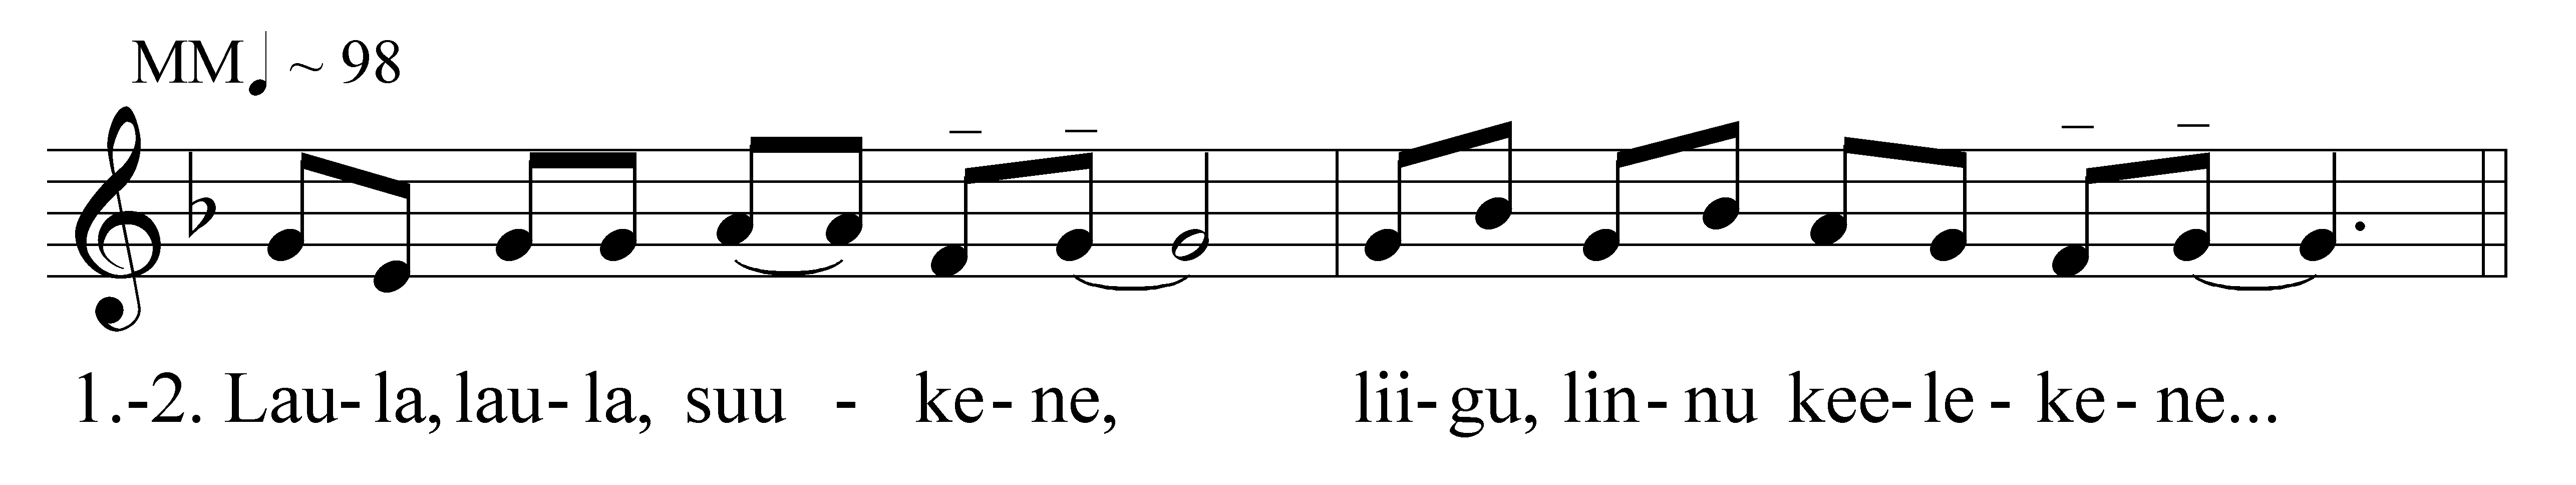
\includegraphics[width=300pt]{figures/055.png}
\caption{Laula! {\it Sing!}}
\label{default}
\end{figure}




The data for this study was sourced at the Estonian Folklore Archives (EFA). 
\citep{orasEstonianFolkloreArchives2022a}.



Until 1948, songs were collected on wax cylinders, then played on a phonograph and transcribed. shellac discs 1936-38, 746 recordings, 
analogue is the biggest collection in the archive, with over 80,000 individual recordings. Open-reel tape, cassette recordings since the 1970s. 
both wax and disc were re-recorded onto open-reel tape in 78-79.
Presently, the sound engineer Jaan Tamm has been working on preserving the earlier tape recordings in digital form for the EFA. WAV files are stored on CD-Rom at the EFA in Tartu, Estonia, while .mp3 and .ogg lossy formats are uploaded to the internet database. 
% collected by Herbert Tampere, Erna Tampere, and Ottilie Kõiva between 1912 and 1966 for the Estonian Folklore Archives in Tartu, Estonia. \\
%
% and   tunes
%the total number of song recordings is over 26,000. Of these, over 11,000 are from the beginning of the 20th century. Tampere did like 2,000 of them..
%
%%
%The need for writing the tunes live during fieldwork has reduced with the availability of analog and now digital audio recording equipment.




Songs for this paper were accessed via The Anthology of Estonian Traditional Music \citep{tampereAnthologyEstonianTraditional2016}. Originally published on four vinyl discs in 1970(\ref{vinyl1970}, the digital version showcases a robust sample of the massive collection of {\it regilaul} in Estonian Folklore Archives. In addition to audio, the  compilation includes  photographs, sheet music, and performer demographics of 98 {\it regilaul} songs and 17 instrumental tunes. 
These songs were compiled in part by Herbert Tampere, an early ethnomusicology field work organizer of the EFA, who along with Erna Tampere and Ottilie Kõiva collected these folk songs. Pictured in \ref{tampy} is a photograph taken of one of the very field trips to record songs studied in this paper. 

\begin{figure}[htb]
\centering

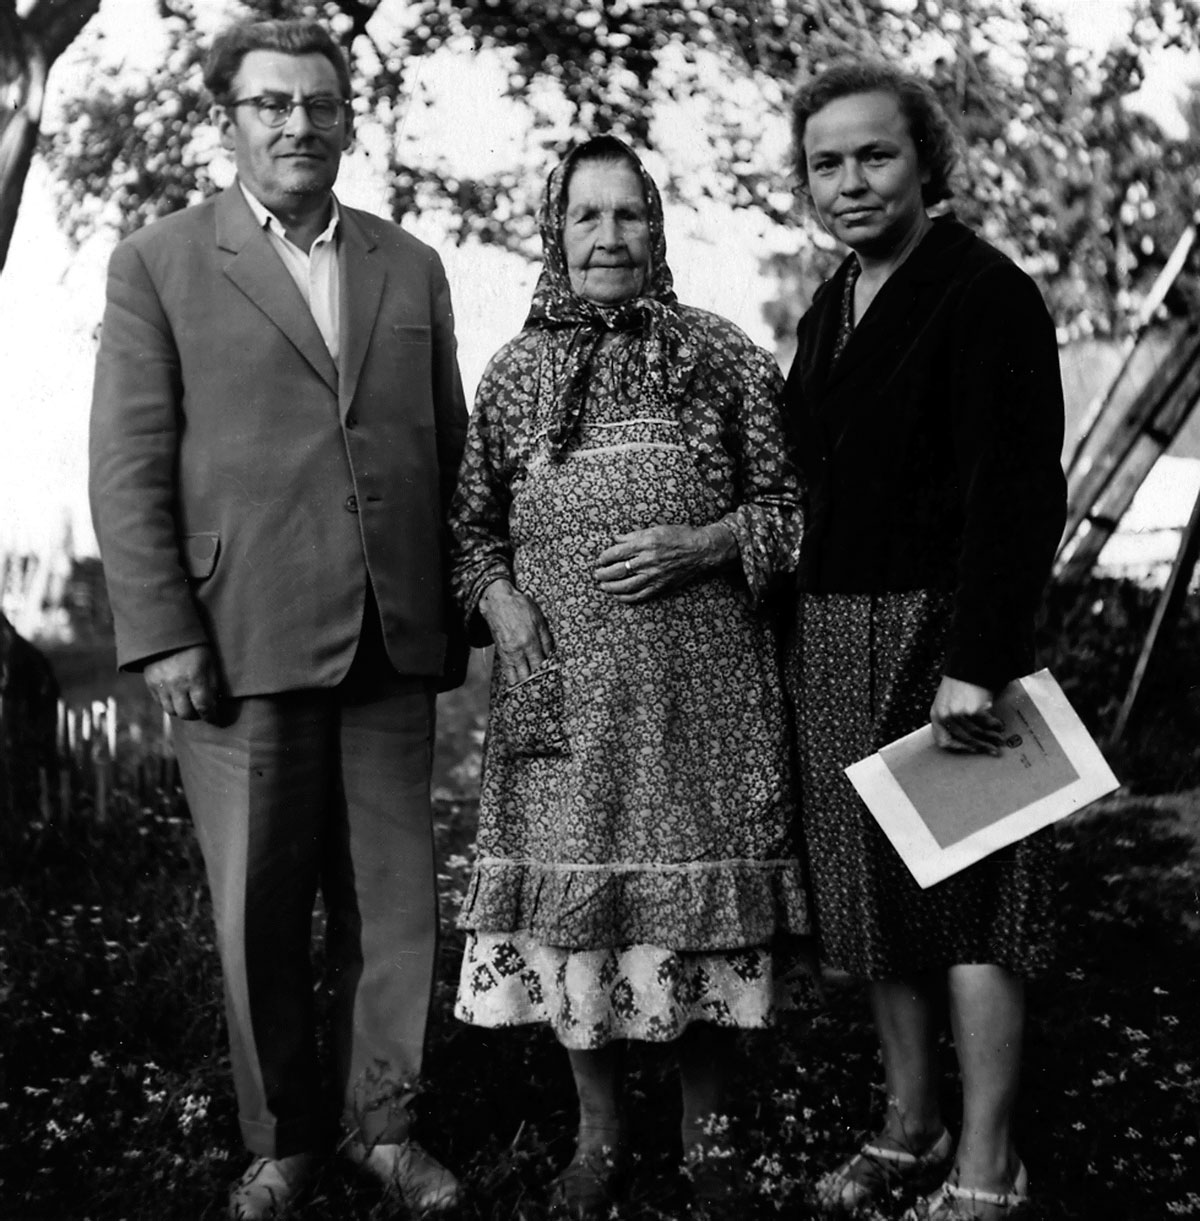
\includegraphics[width=200pt]{figures/Mf_07027_Tampered_Orik.jpg}
\caption{Herbert Tampere on a field trip}
\label{tampy}
\end{figure}


While the ultimate goal is to continue annotation of the entire available corpus of {\it regilaul}, for the initial analysis I chose a sample of songs all belonging to the same regional dialect and recording method. Once several regions were identified as possible candidates, a native Estonian speaker was consulted on the final selection. The nine songs analyzed in this study were all recorded in Parnümaa county from 1961-1966 by Herbert and Erna Tampere. 
% The first criteria is due to the lossy nature of some of the older files available on the site: the online versions are all compressed lossy, so the analog audio originally recorded on tape and then digitized have a higher resolution, even compressed, than songs that have been copied from wax cylinders or shellac discs onto open-reel tape and then digitizing. 


\section{Annotating the Song Audio }



 Each song's lyrics are copied from the site and saved as .txt files in Estonian orthography, each line of the file corresponding to one melody line.  
Audio files of the selected songs are downloaded from the archive in .ogg format, which is the highest resolution of the two lossy\footnote{define lossy} formats available from the digital anthology. Each song is then imported into a Logic Pro X \citep{b131156} session for beat detection, tempo mapping, and trimming. 
To make the tempo map, the session must be set to {\it flex tempo}. From here a beat onset detection algorithm \citep{robertsonBKeeperBeattrackerLive2007} is  given the transcribed bpm and time signature from the archived song data and run on the imported audio file. The result is an annotation of intervals in time, and the bpm for each measure is annotated according to the performance of the song.
The tempo map allows us to document when {\it exactly} in time the particular singer performed a given note, the duration of the sung note, and the acoustic threshold by which the note is defined as ``strong" relative to surrounding notes. The process is informed by the transcribed bpm and time signature included in the anthology. This is beneficial to my purposes in two ways: by accounting for the natural tempo variation in live performance, and by using a consistent metric to determine beat strength acoustically rather than just perceptually.

 From here, a MIDI track is programmed to create a metronome that is the length of a single syllable-note in the song. In most of these, a 4/4 measure contains eight eighth notes, so the metronome track contains four eighth notes indicating the ``ictus" beats. In flex tempo mode, the MIDI track adjusts note and measure length to match the fluctuations in tempo as documented in the map for the song. The metronome and the song audio file are trimmed to match exactly, and the metronome is converted into a textgrid in PRAAT\citep{boersnaPraatDoingPhonetics2022}, where the annotation process continues. 

 


The orthographic text phrases of the song lyrics are then inserted into each phrase interval with a script, and then eSpeak forced aligner for Estonian \citep{duddingtonESpeakSpeechSynthesizer1995} is run on each phrase to the word and phonemic level. Because this forced aligner is trained on spoken, not sung Estonian, the aligner sometimes tries to align words into the signal before they are uttered. In these cases, the word level tier is manually realigned so that it contains all and only the transcribed word, and then the forced aligner is re-run on this word to the segmental level. In the case of a vowel interval containing an obvious silent portion or occlusion, the boundary is manually adjusted to only include sonorant portions of the signal. 
% \begin{figure}[ht]
%\begin{center}
%			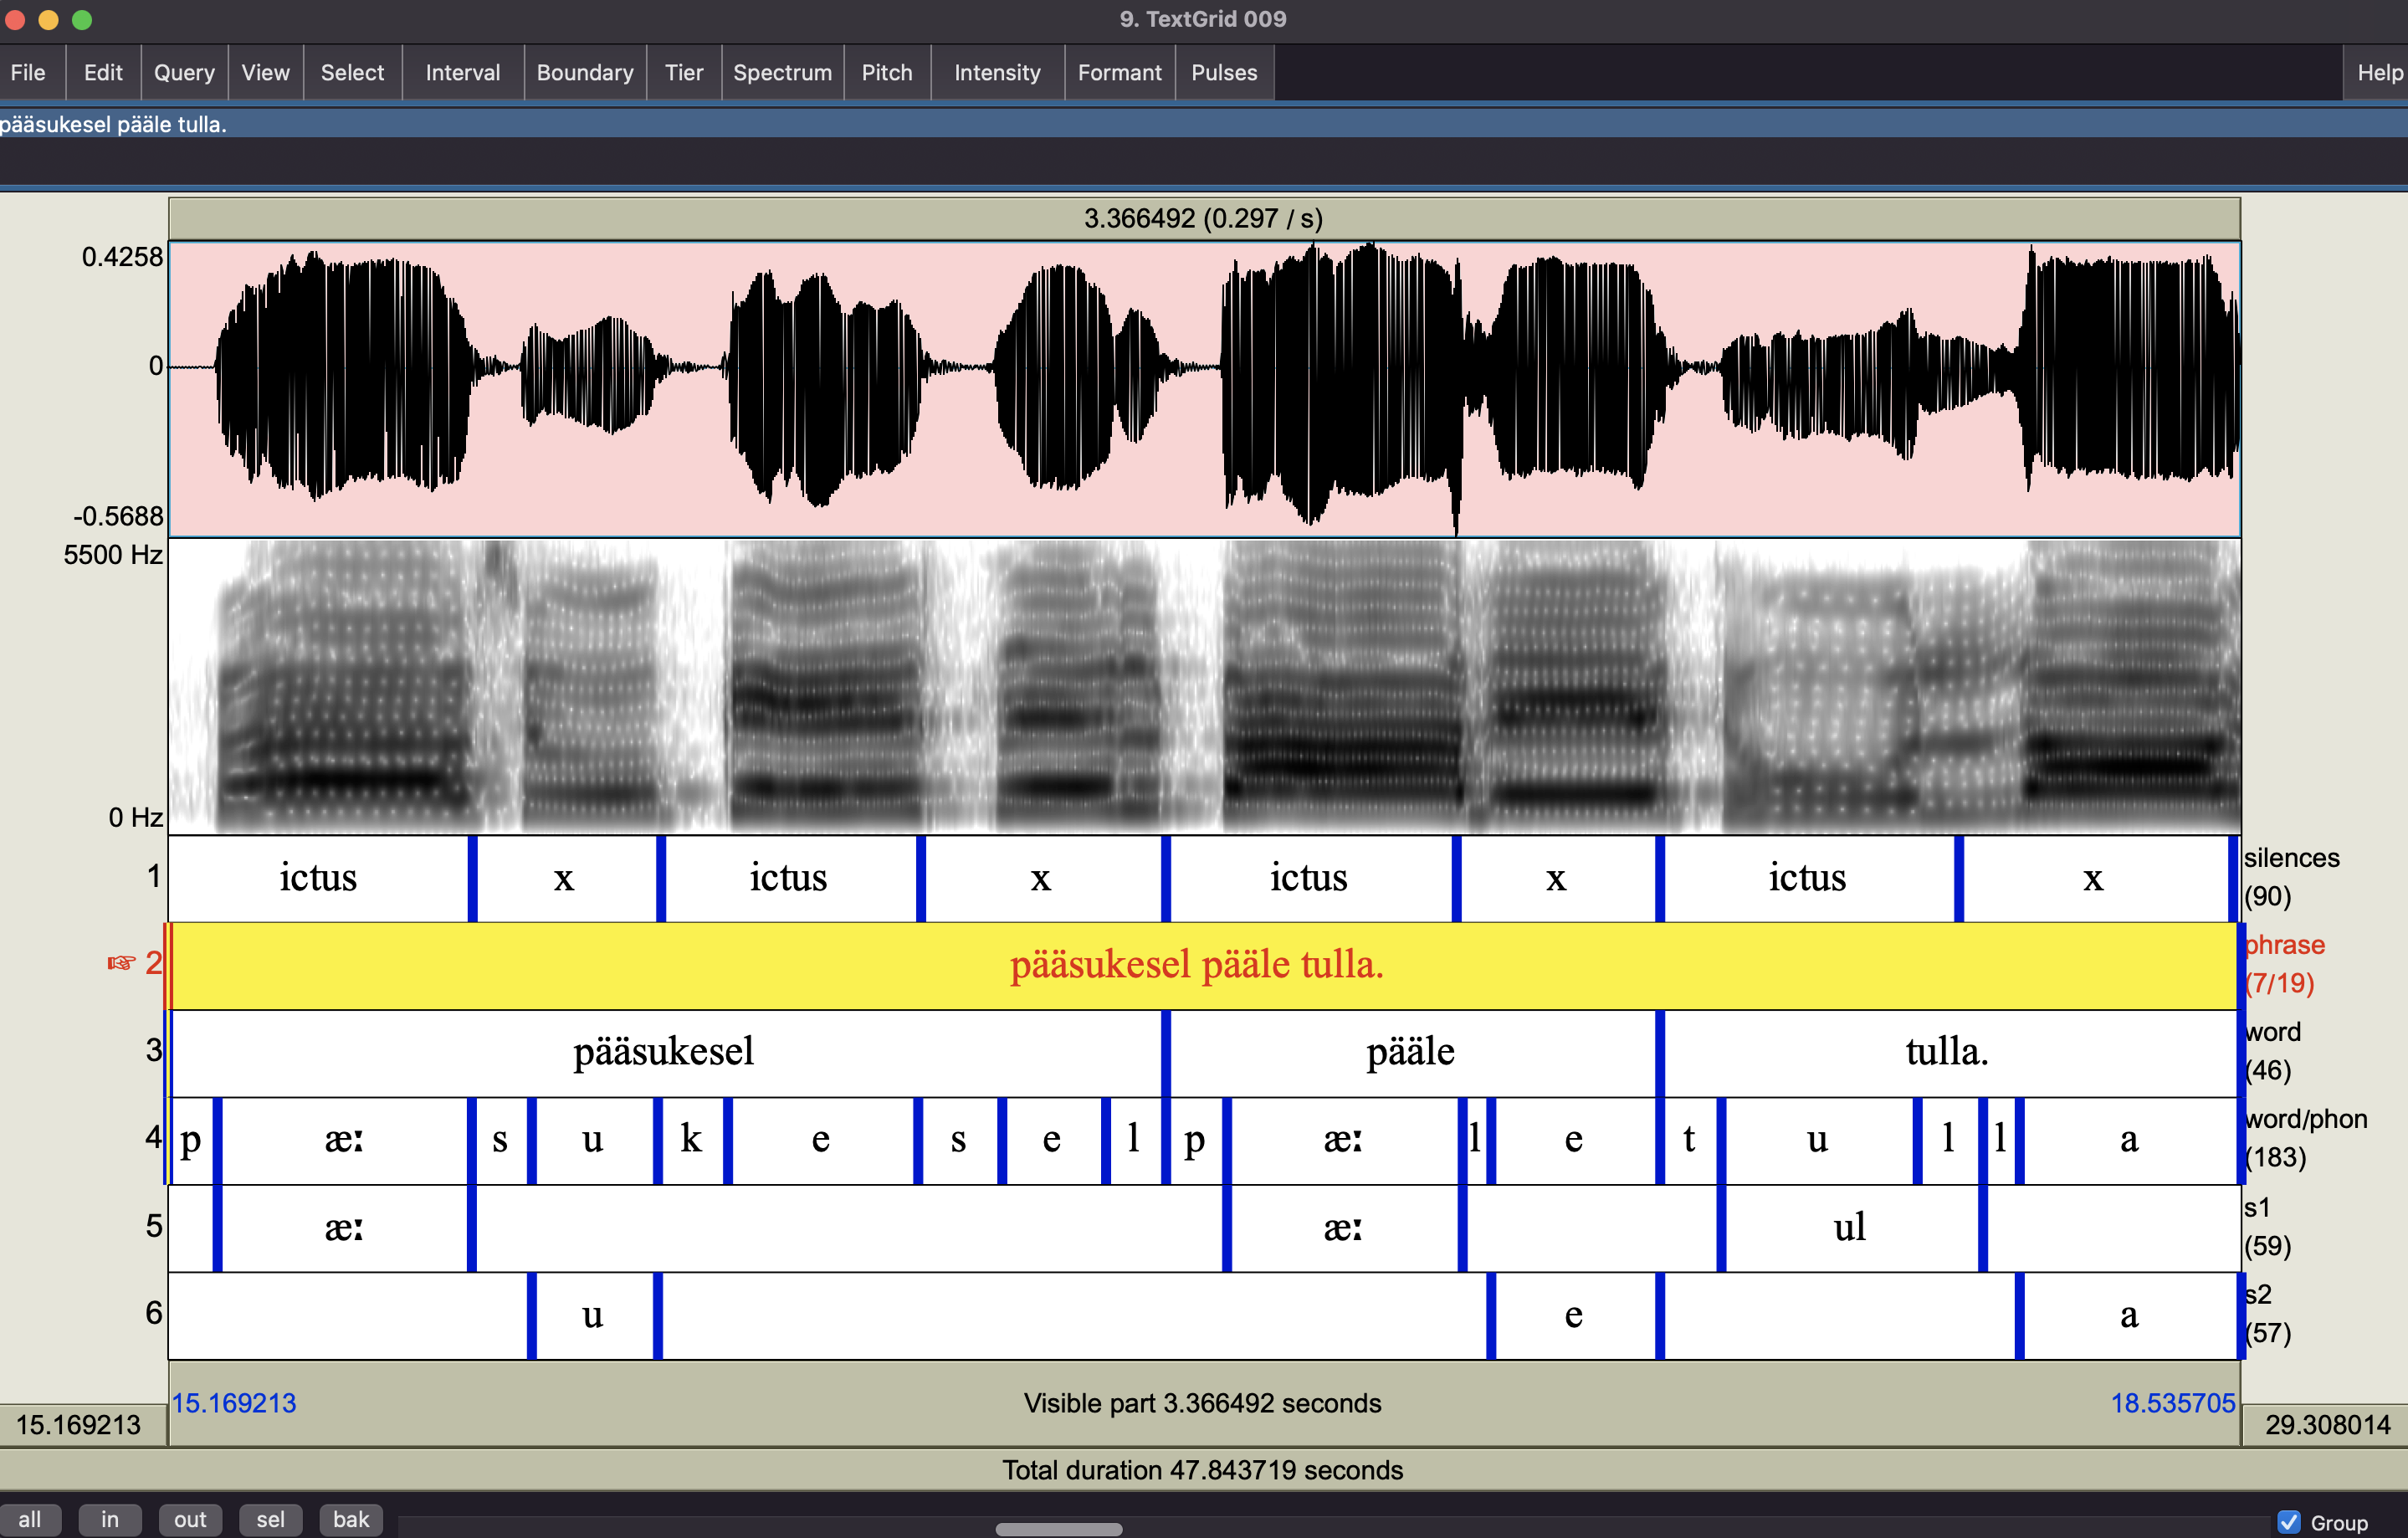
\includegraphics[width=300pt]{figures/phrase_grid.png}
%			\caption{single phrase annotation}
%\label{phrase}
%\end{center}
%\end{figure}
%\begin{figure}[hb]
%		\begin{center}
%			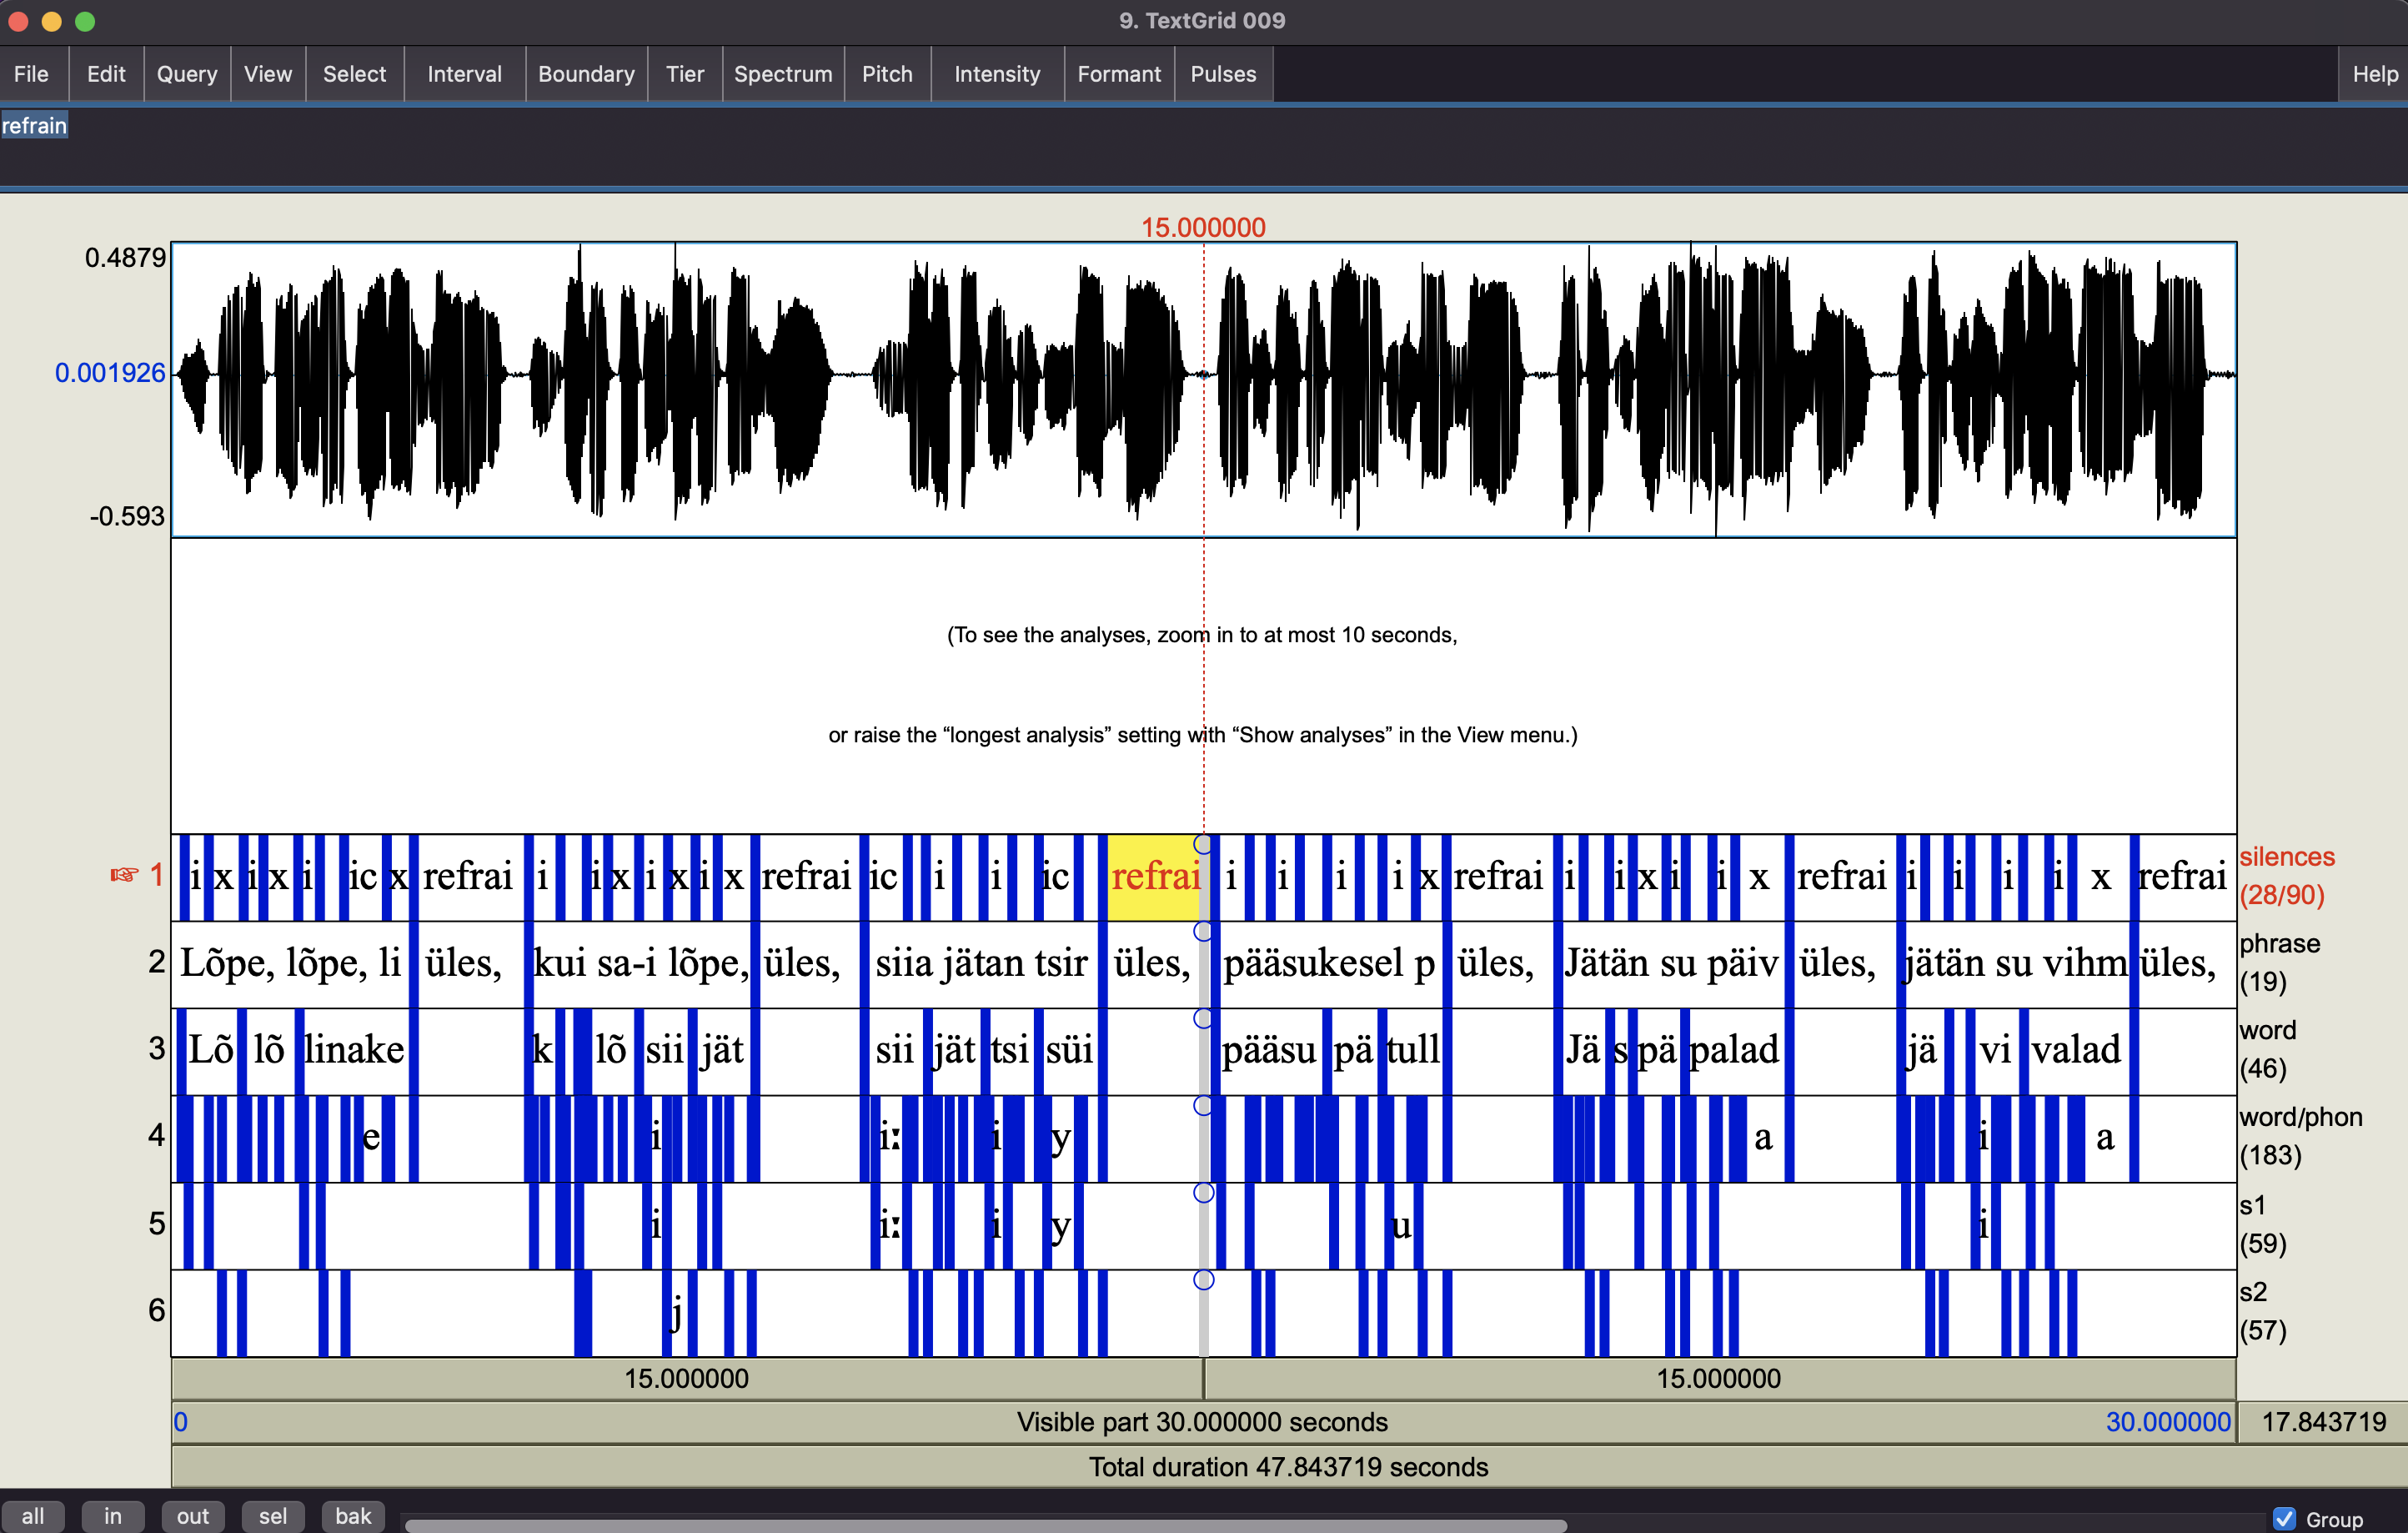
\includegraphics[width=300pt]{figures/big_grid.png}
%			
%			\caption{whole song annotation}
%			\label{songwhole}
%		\end{center}
%\end{figure}
%	
%	 In \ref{phrase} is a completed annotation of a single phrase from a song, and in \ref{songwhole} is an entire song file's interval annotation.

At this point, the audio recording of each song has tiers annotated for tempo and strong beat, verse line phrases, two interval tiers force-aligned to word and phoneme levels, and a separate tier with intervals of the individual vowel segments of interest copied from the phoneme tier.
\section{Assembling the corpus and annotations}
The last step in preprocessing is to integrate the annotation of the song audio with the lexical content of the song. This study accomplishes the task using an open-source natural language toolkit in python called estinltk \url{https://github.com/estnltk} \citep{laur-EtAl:2020:LREC}. Among other things, the toolkit has a robust dictionary of Estonian grammar, including phonetic transcription of syllables with quantity and stress data. 


Thus the data structure of this corpus offers two independent metrics of rhythmic prominence in these songs. From the audio recording and the beat detection, we have an annotation of strong beats based on replicable acoustic measurements, and from the dictionary in the natural language toolkit, we have native speaker intuitions about the lexical weight and prominence in the words of the text. While the stress system is generally predictable, the syllable quantity is not always apparent from the orthography, and not always detectible by a non-native listener. Linguistic descriptions of the Estonian language date back as early as the seventeenth century, but the ternary quantity contrast was not documented until native Estonian linguists contributed their intuitions. The non-native linguists had only described lexical stress \citep{sargEarlyHistoryEstonian2005a}. \\

Using onset detection algorithms such as these \citep{robertsonBKeeperBeattrackerLive2007} in phonetics research, especially in the interdisciplinary field of linguistics and musicology, will be particularly beneficial to answering questions about rhythm: finding a way to bring our intuitions and impressions about ``the beat" together with the acoustic phenomenon. By automating the annotation and measurement process using open source tools, the author hopes to share these machines with those who have similar research interests, and also to invite contributors to the data of this corpus of text data time-aligned to queryable audio signal data. 

\section{Study Design}
\subsection{Questions and Hypotheses}

\subsection{Inclusion Criteria for Vowel Measurements}

Once the annotations are complete, the corresponding text files are aggregated and, the corresponding measurements from PRAAT are concatenated via python using the parselmouth library python interface to PRAAT \citep{parselmouth, van1995python}. 
 I extracted vowel intervals which met the following inclusion criteria. For this study, we are interested in the durations of vowels in initial and pen-initial syllable-notes that are transcribed as isochronous in the melodic transcription. 

\subsection{Statistical Analysis} 
Linear mixed-effects model using lme4 in R \cite{rlme4}. 

For stress and ictus, only q1 and q2 syllables (Q3 never unstressed). \\
for quantity and ictus, only word-level stressed syllables



Design-based formula
Hierarchical Linear Model with group-specific terms

\cite{goodrichRstanarmBayesianApplied2020,brillemanJointLongitudinalTimetoevent2018}

\chapter{Results}
\index{Results@\emph{Results}}%

\section{Quantity Oppositions in Ictus position}


Ternary quantity contrast is only in primary stressed syllables. To analyze vowel duration measurements in all three quantities, a subset of only primary stressed syllables is taken from the dataset. 
At the song level, the kalevala meter avoids short stressed syllables (Q1) in ictus position, preferring Q2 or Q3 (long and overlong) syllables to fall on the beat. In off-ictus postion, short stressed (Q1) syllables are preferred while Q3 avoided.


\begin{figure}[htb]
\centering
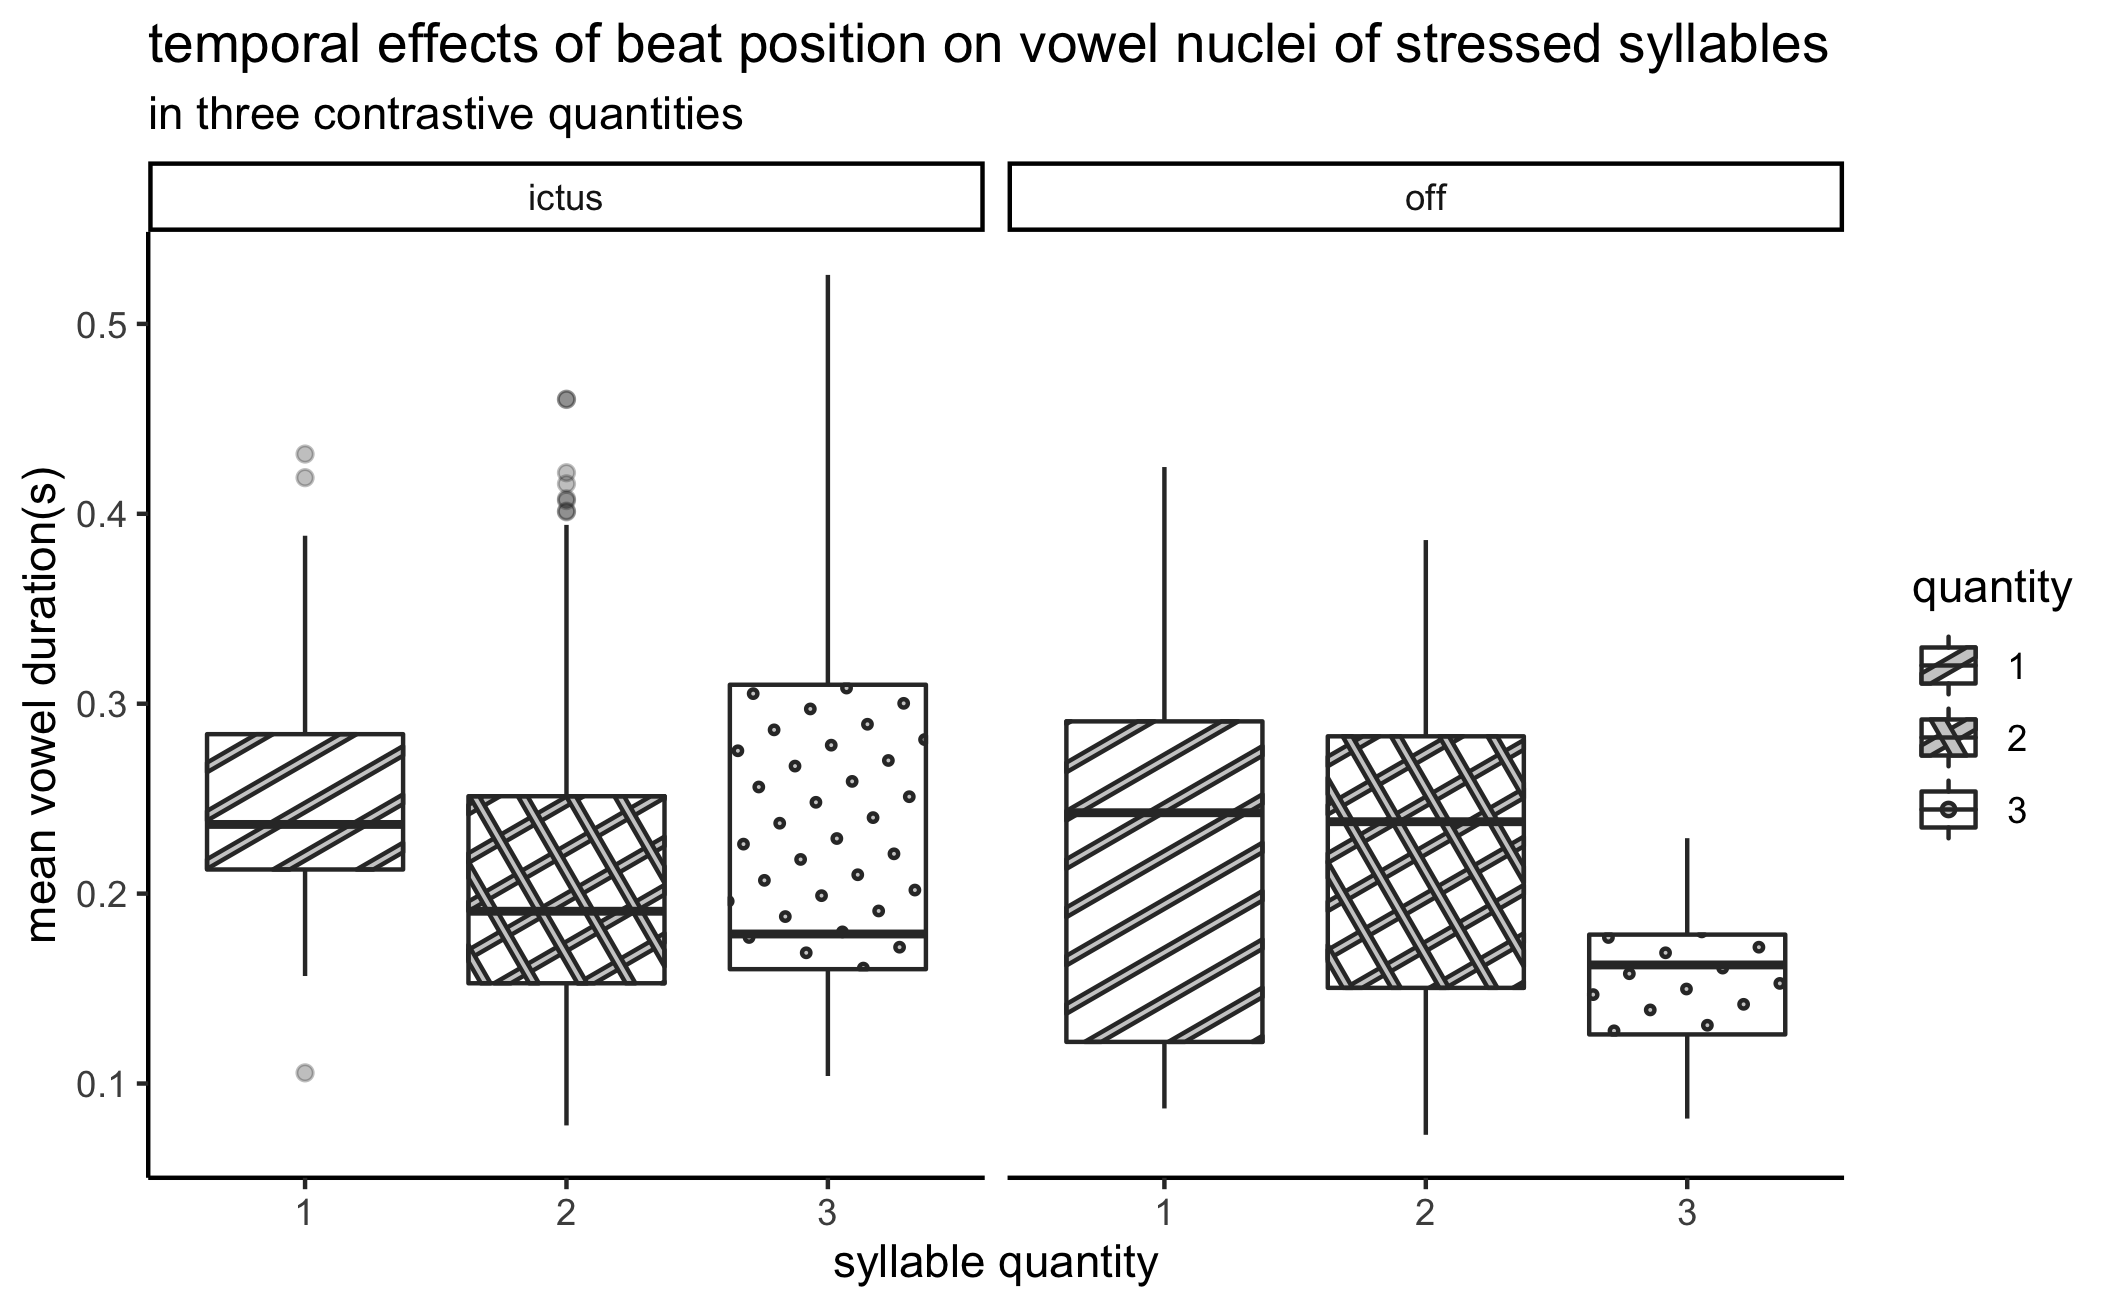
\includegraphics[width =\textwidth]{/Users/sarah/Git/regilaul_project/manuscript/results/q_dur.png}
\caption{density plot of vowel durations in three syllable quantities}
\label{qdur}

\end{figure}
%\begin{wrapfigure}{l}{\textwidth}
%\centering
%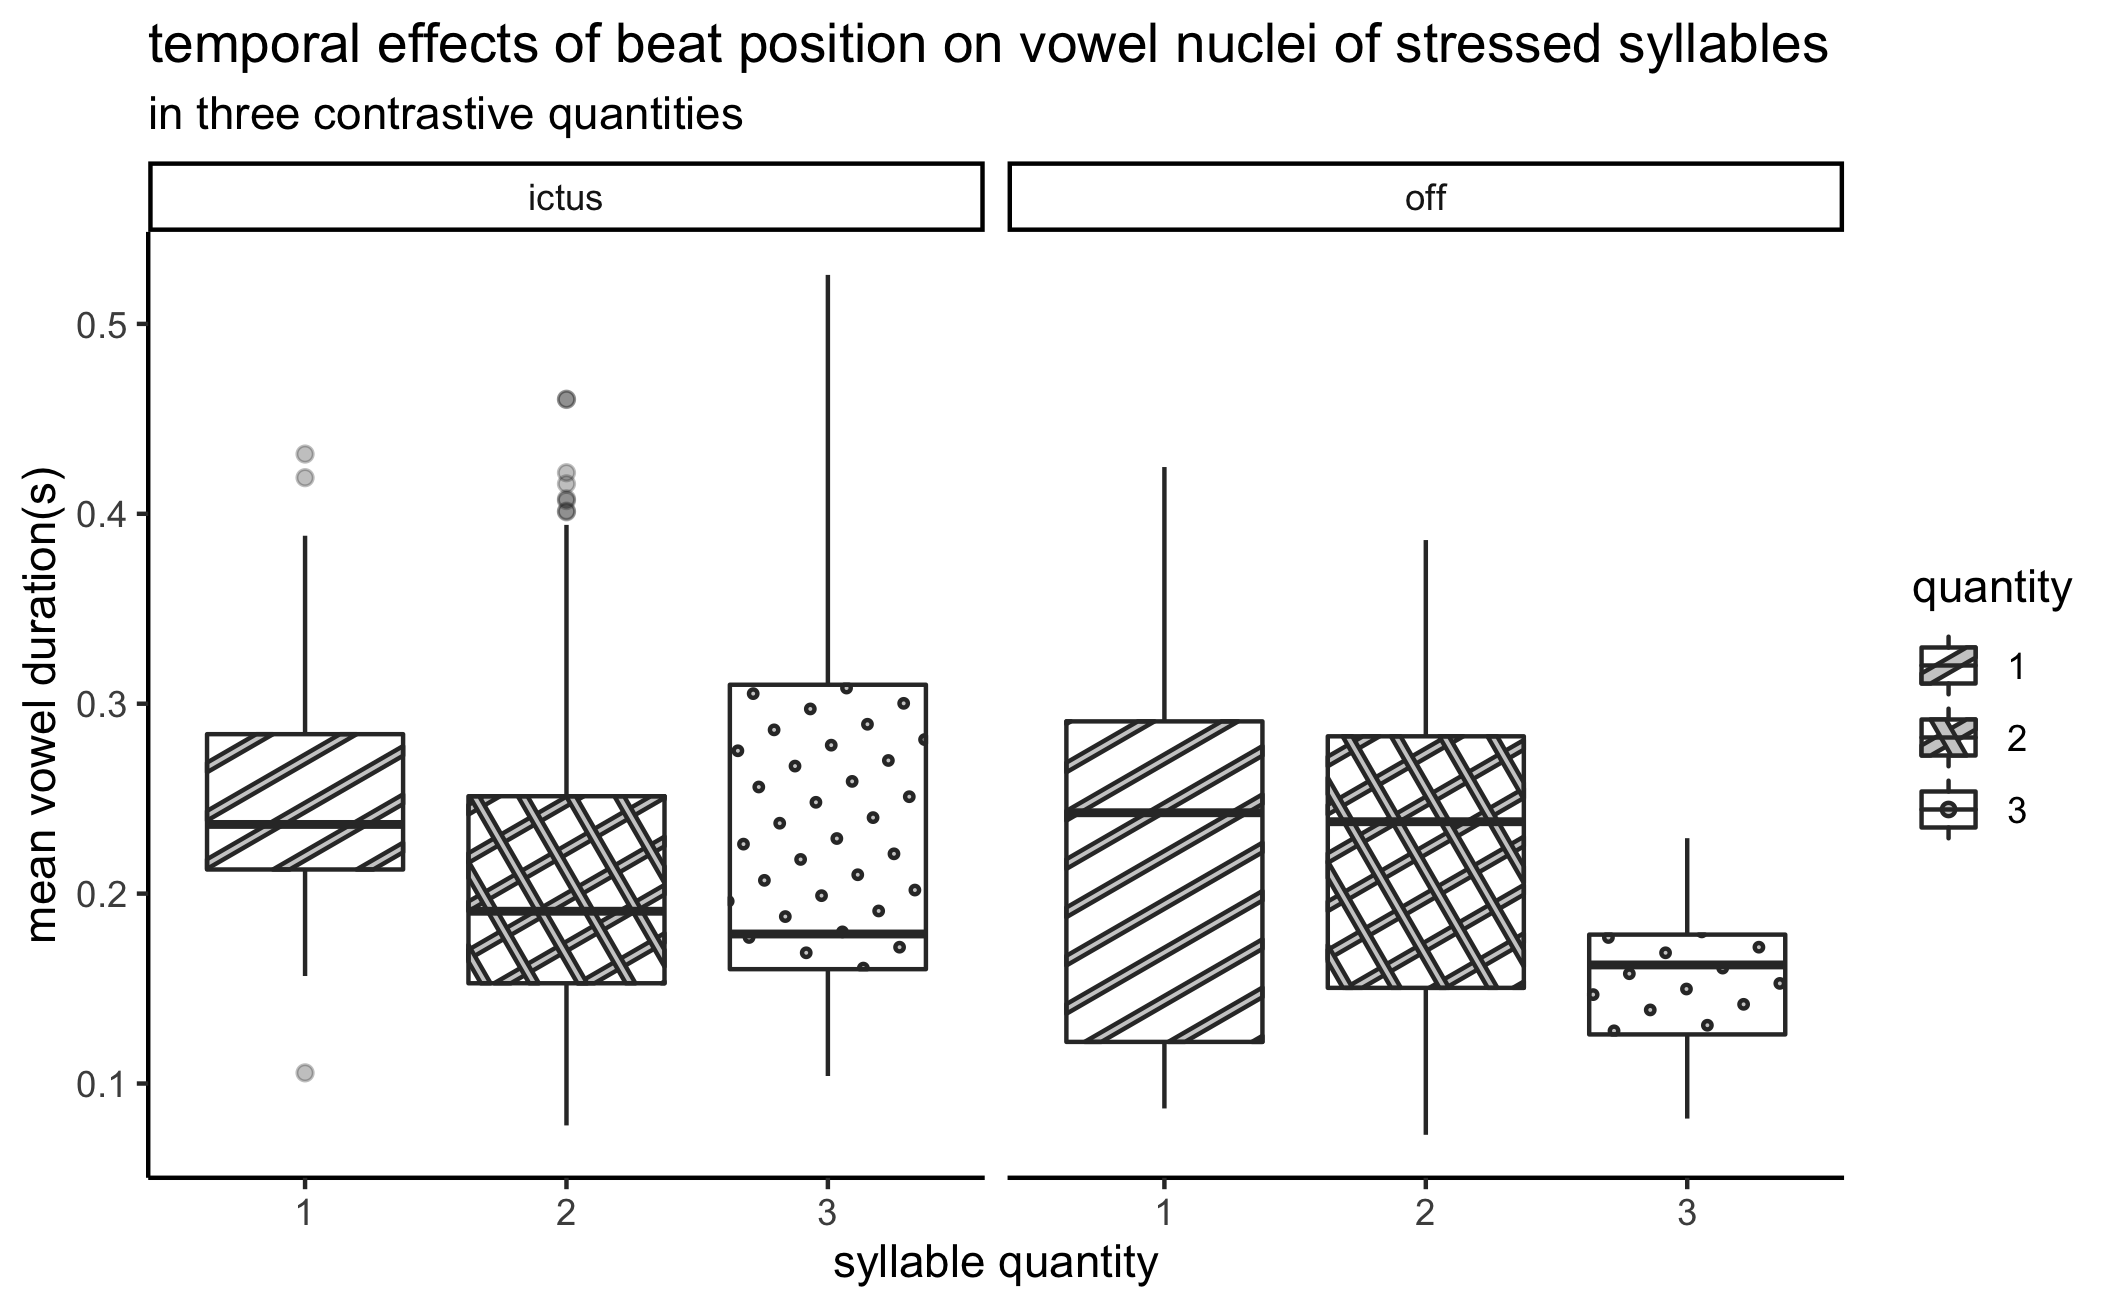
\includegraphics[width =\textwidth]{/Users/sarah/Git/regilaul_project/manuscript/results/q_dur.png}
%\caption{density plot of vowel durations in three syllable quantities}
%\label{qdur}
%
%\end{wrapfigure}


\ref{qdur} shows the vowel durations of all three syllable quantities, grouped by ictus and off-ictus positions in the song. In ictus position, median vowel duration descends as quantity increases, with the greatest difference between Q1 and Q2. Off the beat, a similar descending pattern is evident: however, in this case the largest difference is between Q2 and Q3 syllables. 
 The intercept is set at ictus position, Q1. Findings are significant results for Q2(p<0.001), Q3, and off-ictus positions (p< 0.05). Comparison with null model was statistically significant (p<0.001). For full model output see \ref{qdurfixed} and \ref{qdurrandoms} in Appendix A. In context of earlier findings that the quantity contrast was ``lost" at the syllable level, the decrease in vowel duration as syllable weight increases supports the notion that the contrast is preserved at the segmental level. That is, rather than the full syllable lengthening in duration, the song-level isochrony of syllable-notes results in vowel nuclei shortening to accommodate codas in Q2, and further for geminates and complex codas in Q3. 
 
 
A null model constructed containing only random effects was compared to the design model by two-way ANOVA. Results are significant for the design model (p < 0.001***), and so I reject the null hypothesis. 

These data and analysis support both syllable quantity and ictus as predictors for vowel duration. 



%\begin{equation}
%$$lmer(duration ~ quantity + ictus + quantity * ictus + (1 | song) + (1 | word) + (1 | performer))$$ \\
%
%$$lmer(duration ~ (1 | song) + (1 | word) + (1 | performer))$$
%
%
%
%\end{equation}
\section{stress and unstress}


\subsection{duration}

\begin{figure}[htbp]
\centering
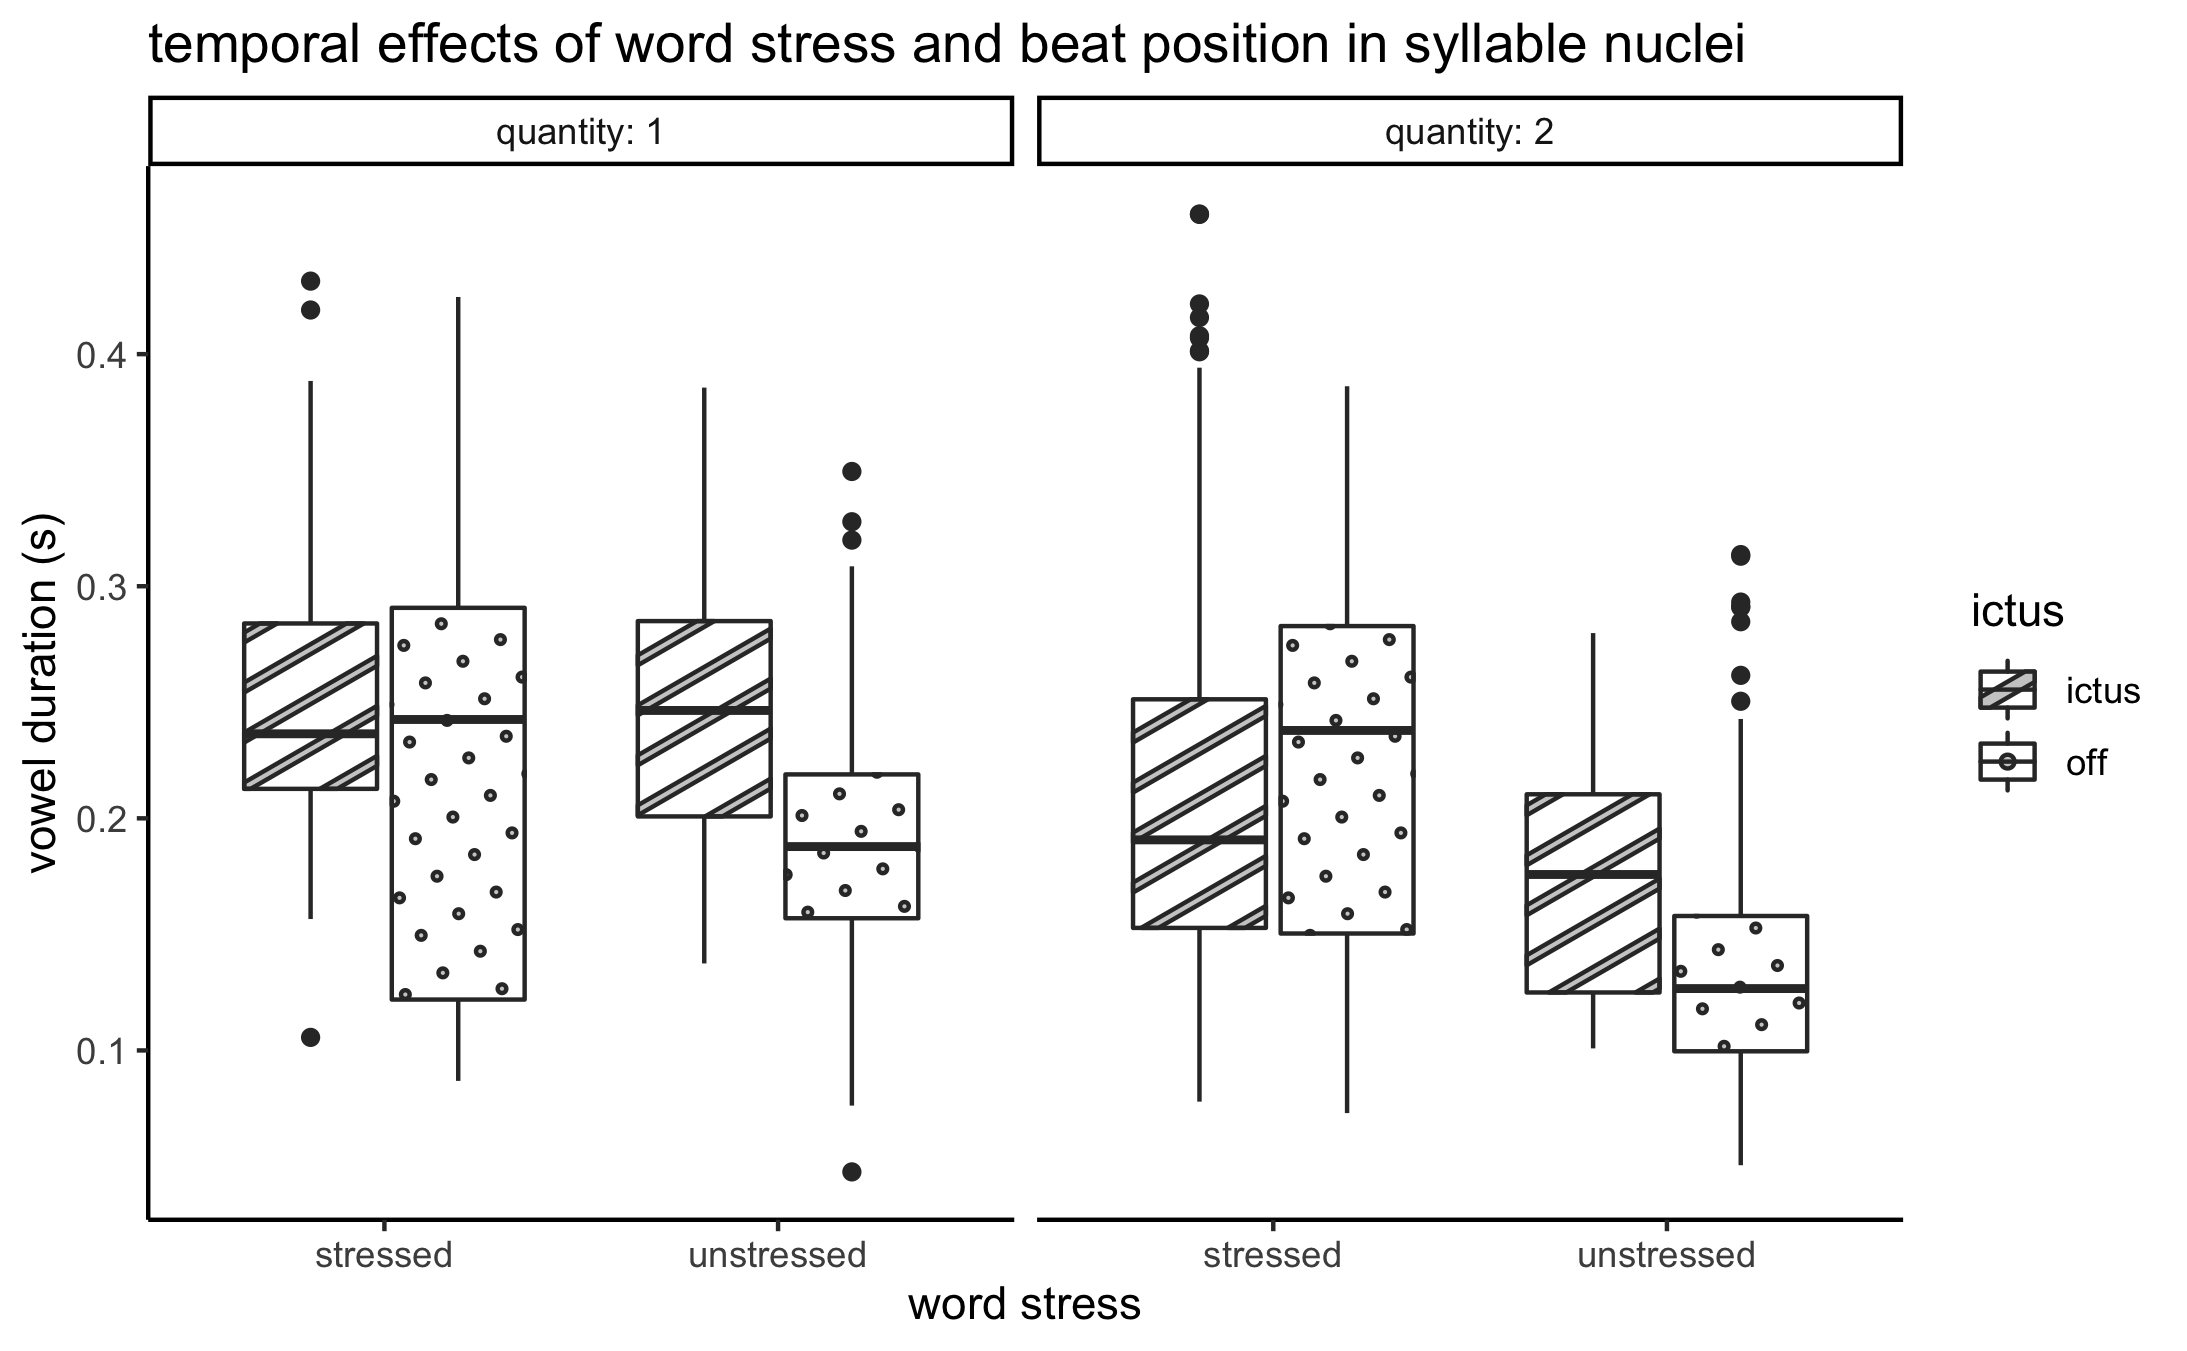
\includegraphics[width = \textwidth]{/Users/sarah/Git/regilaul_project/manuscript/results/dur_density_qfac.png}
\caption{vowel durations of stressed and unstressed Q1 and Q2 syllables falling on (ictus) and off the beat}
\label{durstrick}
\end{figure}

The two graphs in \ref{durstrick} illustrate the distribution of vowel durations in stressed and unstressed syllables falling on and off the beat. In Q1 syllables, ictus position predicts longer vowels in both stressed and unstressed syllables, while stressed syllables are longer overall than unstressed. In Q2, we see longer vowel durations for ictus position in stressed syllables, and higher means for ictus position in unstressed, though the distributions overlap much more here. \\

Linear mixed-effects model results are significant for off-ictus (p<0.05**), stressed (p<0.001***), and Q2 (p<0.001***). 

\begin{figure}[htpb]
\centering
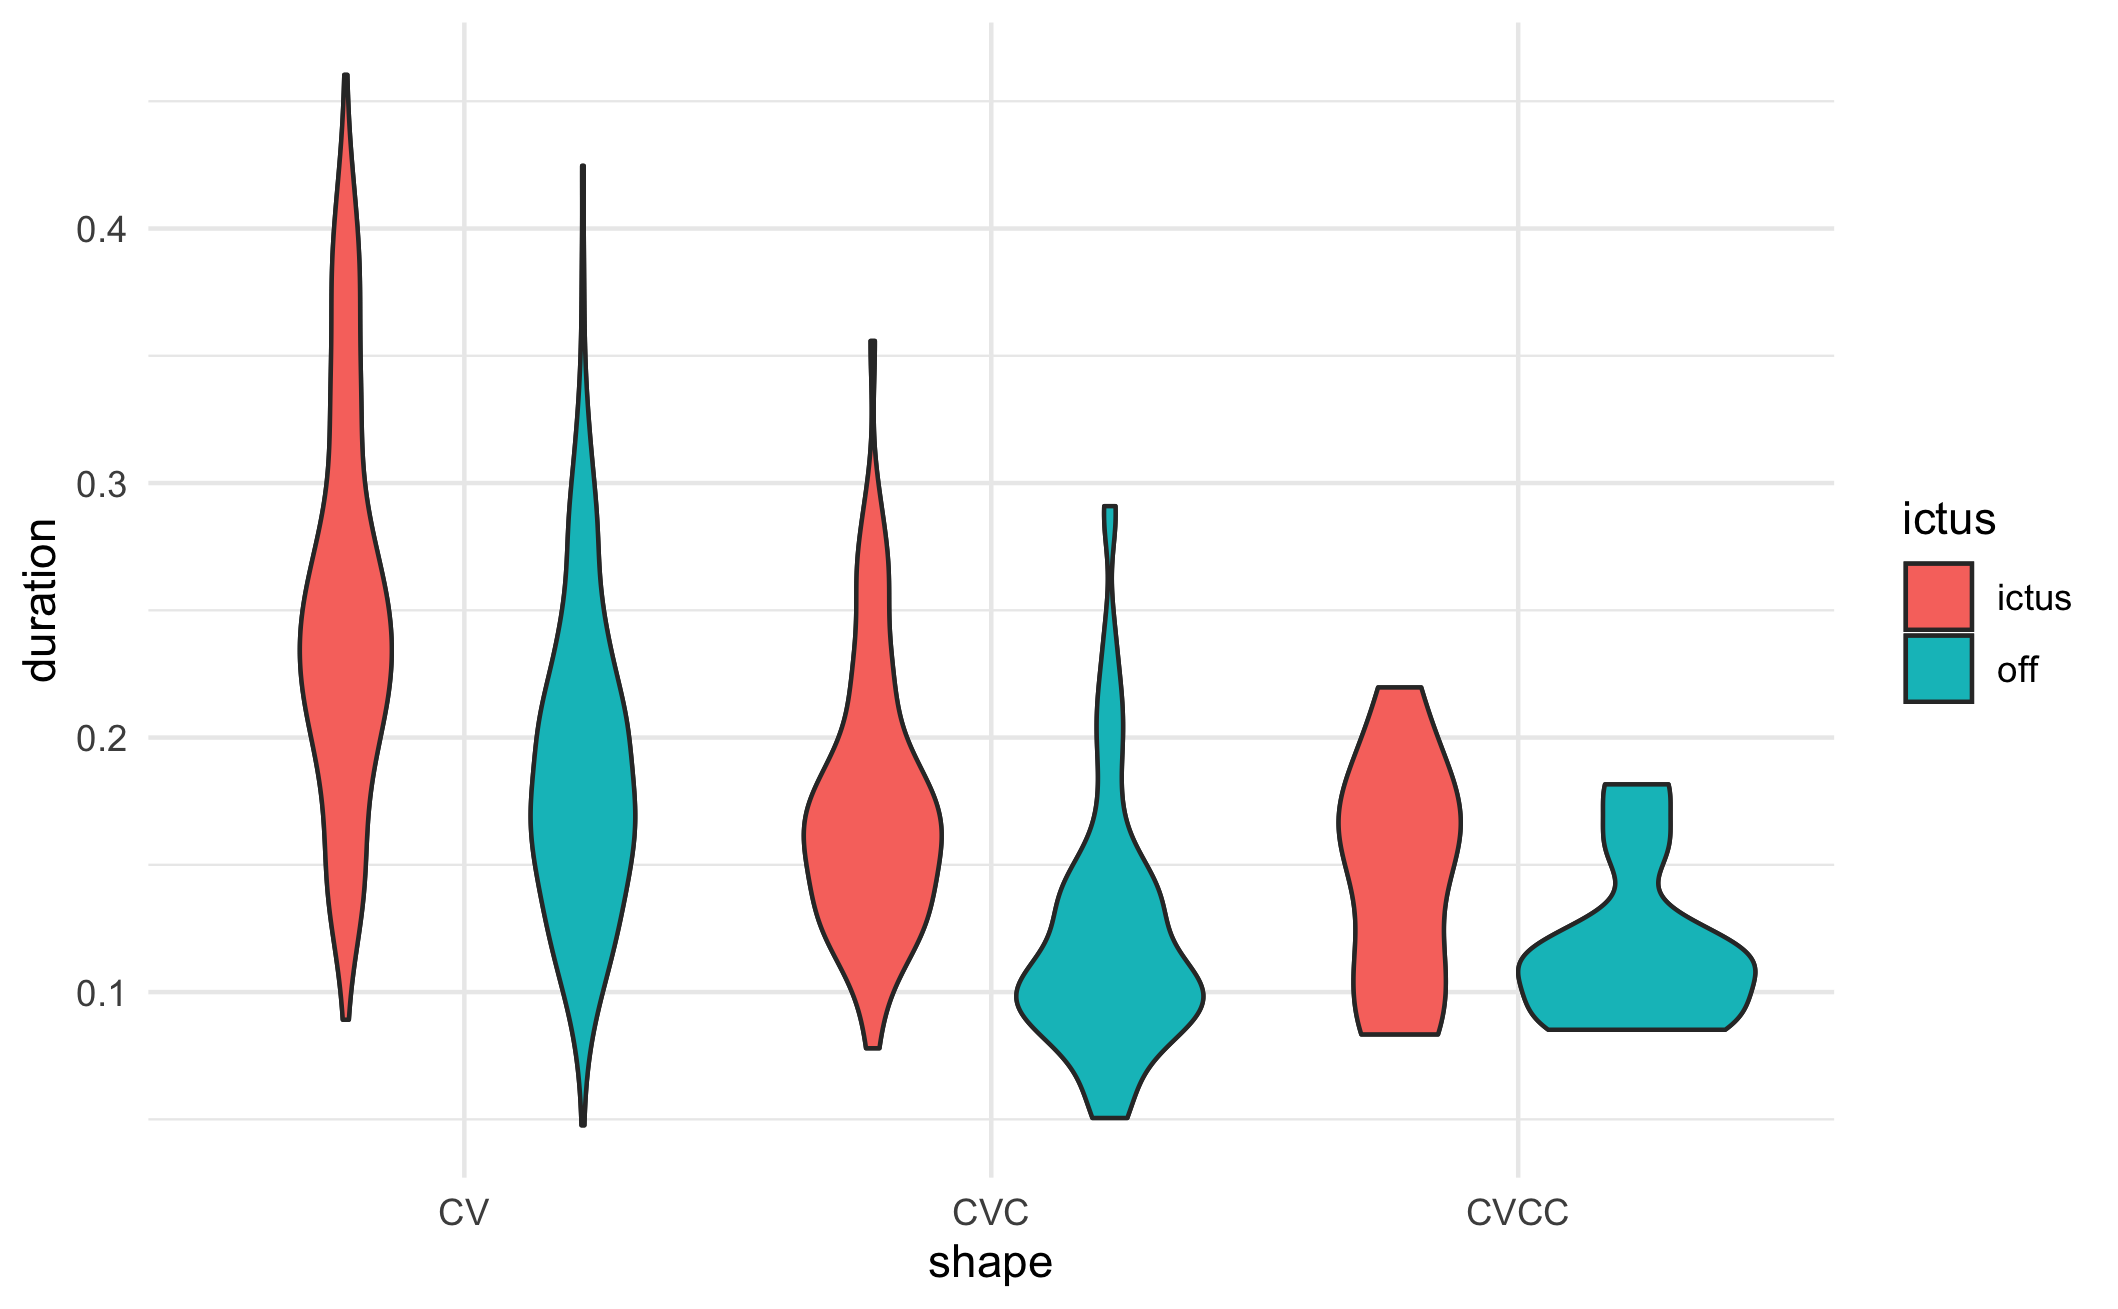
\includegraphics[width=\textwidth]{/Users/sarah/Git/regilaul_project/manuscript/results/dur_shape_ictus.png}
\caption{vowel dur(s) by beat position and syll. shape}
\label{ickdursh}
\end{figure}

Compared to Q1 unstressed syllables in ictus position (the intercept,  off-ictus positions have a negative slope and are overall shorter. Stressed syllables have a small positive slope, indicating longer vowel durations. Q2 syllables have a negative slope, highlighting the shortening of syllable nuclei to accomodate the codas of these syllables. 


\begin{figure}[htbp]
\centering
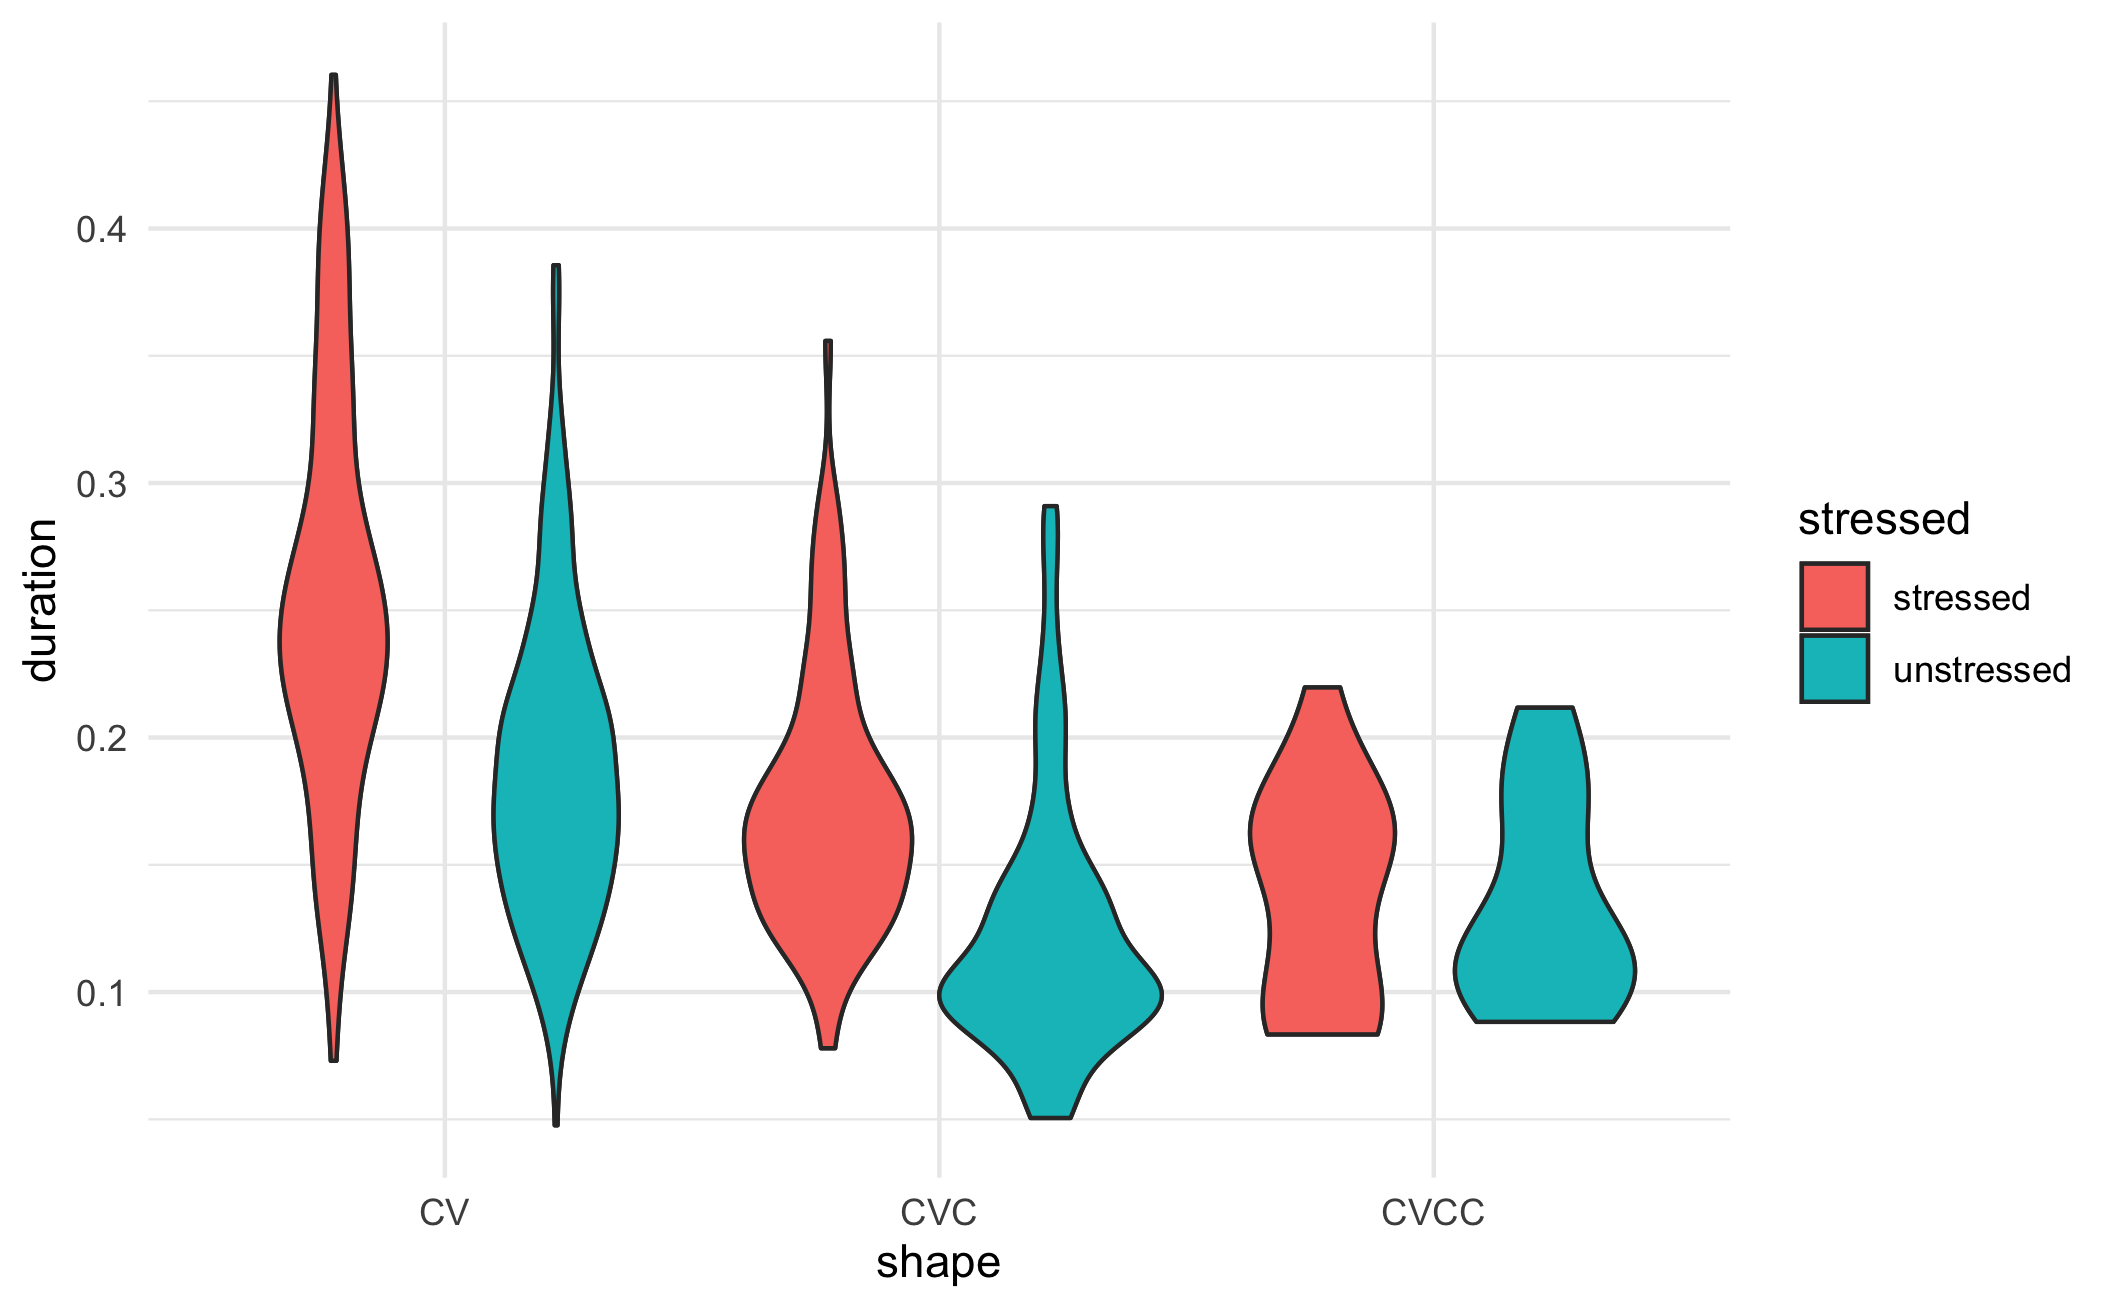
\includegraphics[width=\textwidth]{/Users/sarah/Git/regilaul_project/manuscript/results/dur_shapestress.png}
\caption{vowel dur(s) by word stress and syll. shape}
\label{strdursh}

\end{figure}
Anova comparison of the maximal design model with a null model is also statistically significant (p<0.001***). I reject the null hypothesis: these results support both word-level stress and beat position in song (ictus) as predictors for vowel duration. 

The graph in \ref{ickdursh} illustrates the distribution of vowel durations in different syllable shapes falling on and off the beat. 

A similar pattern can be seen in \ref{strdursh}, where the stressed or unstressed status is shown instead. At both song and word levels of prominence, CV or Q1 syllables are the longest, gradually decreasing in CVC and CVCC, both of which are Q2 syllables.  This further confirms the gradience of the quantity contrast at the segmental level. 



%%%%%%%%%%%%%%%%%%%%%%%%%%%%%%%%%%%%%%%%%%

%
%%%%%%%%%%%%

\subsection{Vowel Dispersion}
A subset of the Q1 and Q2 vowels used for duration measurements above is taken,  containing only those five vowel phonemes which occur in both stressed and unstressed syllables at the word level: \[a, e, i, o, u\]. The total number of vowels in this set is {\bf N}.
To account for physiological differences between singers, vowel dispersion is calculated as the euclidean distance of each token from the respective singer's vowel center in the (F1, F2) space. 


\begin{figure}[htbp]
\centering
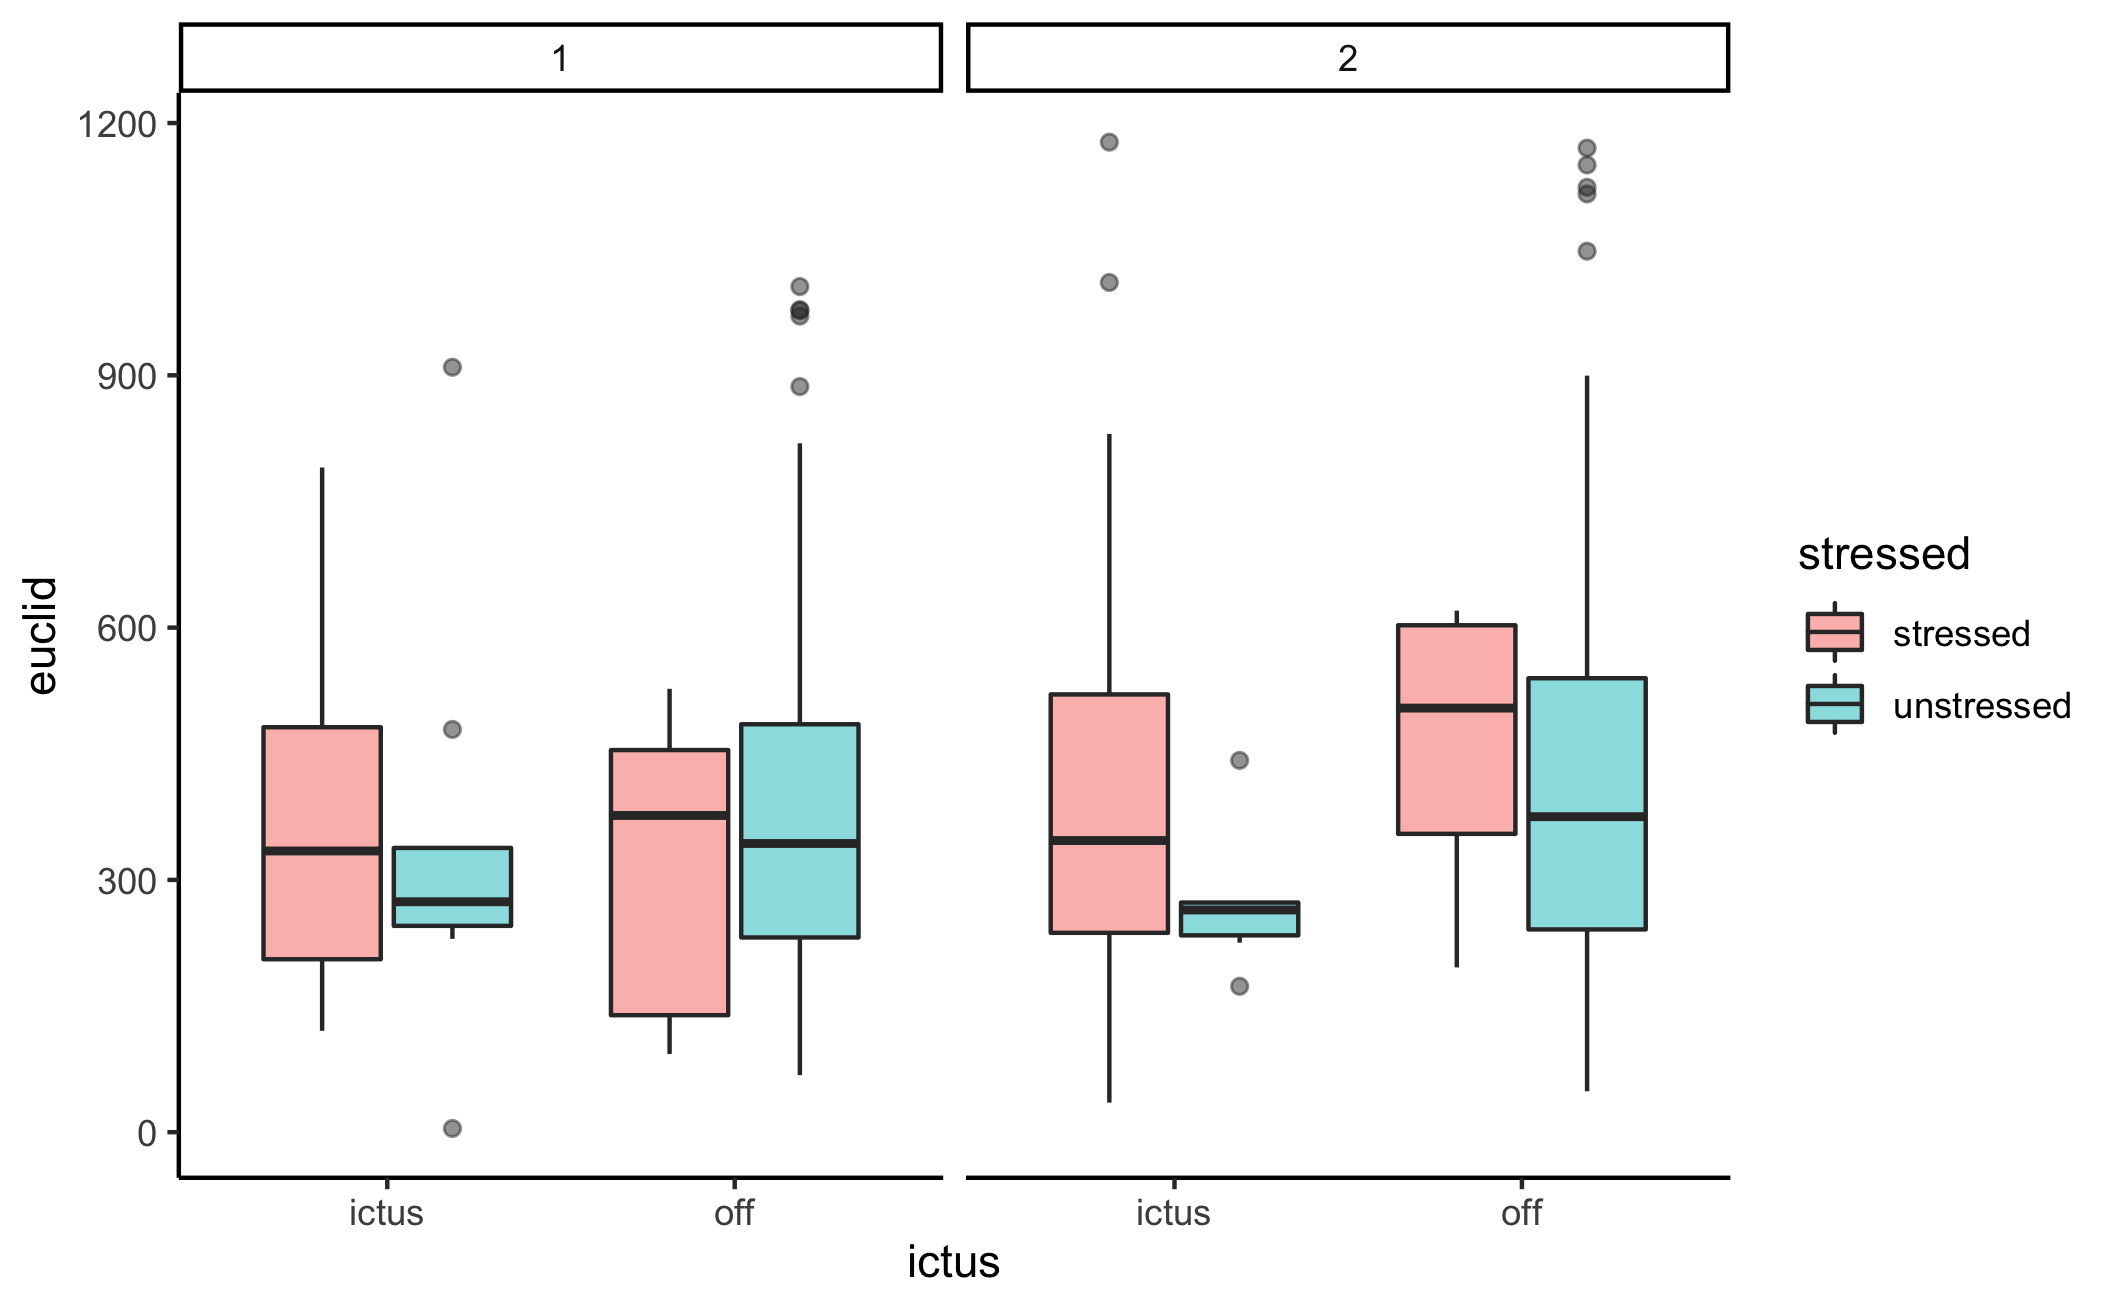
\includegraphics[width=\textwidth]{/Users/sarah/Git/regilaul_project/manuscript/results/space_strictus.png}
\caption{euclidean distance of vowels in stress and ictus}
\label{spcstrick}

\end{figure}
A pattern is marginally visible in the two graphs  \ref{spcstrick}, faceted by Q1 and Q2. Notice that in off-ictus position, vowel dispersion means of stressed syllables are higher than those of stressed syllables in ictus position. This indicates that stressed syllables falling off the beat are being compensated for their shortened vowels by way of increased articulation of quality. This pattern, however, doesn't shake out as statistically significant in the model. \\
A linear mixed effects model for vowel dispersion is constructed, but only the uninterpretable intercept shows significance. 
Comparison with null model is not statistically significant. Thus in the case of vowel dispersion, we fail to reject the null hypothesis. This could be due to the relatively smaller size of the data subset. 



%\chapter{Discussion}
\index{Discussion@\emph{Discussion}}%

\section{Temporal Prosodic Features Crystalized at Segmental level in isochronous syllables}

These results support the hypothesis that prosodic timing modifications resulting from the synchronization of independent rhythms (in this case, syllables and notes into syllable-notes) do not result in the subordination of one system to another. In this case, when syllables and notes become one timing unit, the temporal acoustic correlates often found at suprasegmental levels (syllable, foot, word) are found at the segmental levels. 

This interaction is then more analagous to entrainment of two independent rhythmic systems than to language being forcibly pigeon-holed into the metrical structure of music. 


%\section{Vowel Dispersion}
%Results for the predictive power of ictus and off-ictus, stressed and unstressed syllables and vowel space dispersion were not significant. The patterns that seem to emerge visually in the graphs of distributions suggest that the situation might be ameliorated by increasing the dataset. For this measurement, there were fewer available tokens than for vowel duration, and therefore less statistical power. Further examination is needed to determine whether or not the observed pattern is simply lacking in power or whether the premises that lead to this hypothesis are missing something entirely. 


\section{Future Studies} 

This study used a sample of nine songs and three singers, all recorded in the 1960s. Annotation has already begun on the remaining songs that fit into this sample's criteria: In total, there are seventeen songs and seven singers from Parnumaa county recorded in the 1960s.
% Increasing the size of the audio corpus would facilitate exploratory analysis in countless dimensions of music and language, and also shed light on the issue of vowel space unresolved here. 
Several of the singers featured in this sample set were also recorded speaking. Annotating their natural speech would provide a valuable contribution to the song corpus, as findings from the songs could be compared with speech of the same person.  

Extending the findings of vowel duration and the ternary quantity contrast has several obvious paths: synchronic analysis of with song samples from the same approximate time period but differing according to region, or even language: several other Balto-Finnic families have a trochaic tetrameter folksong tradition. Diachronic analysis with song samples of same singers in the same region at different points in time is another possibility with data from the Estonian Folklore Archives. Both these goals are achievable only with the continued annotation of the corpus of regilaul, which is quite demanding work. As I continue to build this corpus, I am also actively exploring ways in which to automate the process. The inclusion of beat tracking software eliminated much observer subjectivity, and also facilitated the forced-aligner: by automatically grouping verse lines into measures, the aligner was given phrase groupings to synthesize and compare, rather than attempting to align the entire song in a linear fashion. However, as the forced aligner used here was made specifically for speech, one way to improve the accuracy of the forced aligner (decreasing manual adjustment of annotations) would be to train a the aligner on sung material using supervised machine learning. As I plan to continue with the annotations either way, I can use the corrections I make as training material for the algorithm, with the hopeful result that the forced-aligner will eventually reach some threshold of accuracy, voiding the need for manual adjustments. 

\section{ML plans outline}
%Kaldi: uses DNN (Deep Neural Net) rather than linear model like MFA (montreal forced-aligner). 

%https://www.kaldi-asr.org/doc/
%https://www.eleanorchodroff.com/tutorial/kaldi/index.html

for several/general uralic languages \citep{leinonen2021}. 
Would be good to try for other runosongs! 

%https://github.com/lingsoft/aalto-kaldi-align-elg

for Estonian specifically \citep{ratsep2022}
\section{Conclusion}

This study examined fine-grained acoustic-phonetic features of Estonian prosody in the context of traditional folksongs known as regilaul. The data support the hypothesis that duration contrasts inherent in the ternary quantities of Estonian are still present at the segmental level, even after undergoing modification to fit syllables into isochronous notes of the song. The data also supports that the durational correlates of word-level stress are also crystallized and evident at the segmental level, so while it isn't lexically contrastive, the role of primary stress and unstress to mark word boundaries in spoken Estonian is still present in sung Estonian. 
%Vowel quality patterns were measured but not significant for this dataset. 

This indicates a relationship more akin to the collaboration of two independent rhythmic systems rather than one rhythmic system dominating the other. Combined with the fact that any regilaul text can be sung to any existing regilaul melody brings into question whether {\it spoken} metrical verse text is truly independent of the temporal constraints of the musical meter they are made with, or somewhere between language and music. 

%\chapter{Conclusion}
\index{Conclusion@\emph{Conclusion}}%

%Vowel Duration: \\
%We failed to reject the null hypothesis for vowel duration: while the song level does dominate the temporal domain, there is an inverse relationship to vowel duration and word-level duration contrasts for Q1, Q3, and stressed syllables. So while the song always wins, there is clearly something else going on. It is possible that it is as simple as note-syllable isochrony, and the vowel decrease is simply an accommodation to give the ictus level the appropriate duration syllable. 
%
%Vowel Space: \\
%
%After confirming that song position is the dominant hierarchy for temporal constraints, we continue on to see how vowel space plays out in different levels of prosodic prominence. We are able to reject the null hypothesis with data to support a clear relationship between prominence and vowel space, this time at both prosodic levels (song and word.) This suggests that for the song, ``preserve contrast" ranks lower than the temporal constraints, but that so long as the strong positions in the song are satisfied, prominence can be indicated by vowel space at multiple levels of the prosodic hierarchy.  





%\chapter{Background}
\index{Background@\emph{Background}}%is

\section{Meter and Rhythm}

Given the interdisciplinary nature of the research questions, an earnest attempt was made to find a suitable intersection in the literature from which to approach this. Computational studies of music, acoustic-phonetic studies of Estonian both proved useful, but it was in the specific domain of metrical prosody that problems arose. 

For one thing, the oft-cited \citep{essensPovel1985} offers a definition of metrical  temporal patterns according to what they call "integer ratios" such as 2:1, 3:1, etc, and nonmetrical patterns corresponding to "non-integer ratios," which they offer in the forms 1.5:1, 2.5:1, 3.5:1, and so on. This definition defies the principles of elementary number theory in several ways: 1.5:1, 2.5:1, and 3.5:1 are equivalent to 3:2, 5:2, and 7:2, respectively. In their simplest form, it is clear that they are in fact ratios composed of prime integers. Indeed the term "non-integer ratio" is a pecuiliar one, as integers are a subset of all rational numbers, who are defined by their representability as ratios. Outside the set of rational numbers are the irrationals: but if we are cognitively restricted to timekeeping with simple ratios only, we should have considerable difficulty reading time from a clock: the ratio of a circle's radius to its diameter is the transcendental \pi.  

The results of \citep{essensPovel1985} indicating subjects' difficulty in repeating these patterns compared to others can be explained by the fact that the stimulus design did not offer complete repetitions of this pattern, due to the authors choice to represent the prime ratios in this way. It also violates a basic understanding of human chronobiology more generally: extending their conclusions with respect to the 7:2 ratio would predict that the expression ``same time next week" should be incomprehensible. 


This brings forth another issue which I think is the result of a microscopic view of rhythm. There is a notion in the literature of timekeeping relying on "inducing" some sort of internal clock. This elides the fact that we are rhythmic biological entities. Our minds do not "make" a clock for external stimulus: we {\it are} the clock. Keeping time with external rhythms is the result of entrainment of our own rhythm to those in our environment. \citep{chronobiology, musicCognition} 

From the perspective of a percussionist, there is no issue with complex or odd meters. A novel pattern may be more difficult than a familiar one, but only while it remains novel: you might not produce a piece in 11/4 perfectly the first or second time you try it. Once had, it can be produced on demand: in synchronisation with others, and seemingly from ``thin air."







%\section{Phonetic Realization of Trochees in Spoken Verse} 


%In order to discuss questions regarding word-prosodic Estonian rhythm in the context of musical rhythm, I define the acoustic and perceptual notions of both domains, beginning with musical meter more generally, and continuing into the Estonian language and relevant verbal art forms. Once established, I then give a thorough overview of
% previous research in the domain of song and word prominence in Estonian {\it regilaul}. All this culminates into the research questions and hypotheses that are the subject of this paper. 
%\section{musical meter}
%
%
%
%
%\section{Estonian Word Prosody}
%
%
%
%The rhythmic organization of song integrates the prosodic structure of the language with musical rhythmic principles \citep{palmerLinguisticProsodyMusical1992}. 
%
%Duration can be a phonetic correlate of stress, and it can also be independently contrastive at the segmental level \citep{lehistePhoneticsMetrics1992}. 
%
%
%Whether there is a correlation between poetic metre and the prosodic structure of a language.
%
%
%
%
%
%\citep{lehistePhoneticsMetrics1992} investigated the actual phonetic realization of different metres in different languages, finding evidence for one language's trochee, for example, to be realized in a way that is systematically different from another language's trochee. 
%
%Ross found vowel reduction in certain notes, but they were all unstressed, off-ictus for that song\citep{rossFormants90}.
%
%
%The role of primary stress in Estonian is described by Ilse Lehiste as {\it identificational} rather than contrastive \citep{lehistePhoneticsMetrics1992}. In other words, there are no stress minimal pairs at the lexical level, so the prominence cue is to indicate the onset of a new word. This is sometimes also called {\it demarcative} stress.
%
%
%
%Three proposed levels of stress: primary stress, unstress, and secondary stress. \citep{lippusAcousticStudyEstonian2014a}
%
%Primary lexical stress in native Estonian words is fixed, falling on word-initial syllables. 
%\cite{eekmeisterUralica98}
%\begin{exe}
%\ex \gll laul-da \\
%	{[ˈlɑuːl.dɑ]} \\
%	sing-\Tr{} 
%	\glt	`singing'
%\ex 	ööbik \\
%	{[ˈøː.pikː]} \\
%	nightingale.\Nom{} 
%	\glt`nightingale'
%\end{exe}
%
%Estonian has three syllable weights, also called degrees or quantities, that are contrastive in primary stress position. The first degree or Q1 is described as short, 
%In \ref{quant_cont}, we see two minimal pairs illustrating this contrast. 
%
%This ternary contrast has long been the subject of debate in the phonological literature of metrics: Q3 syllables have been analyzed both as a monosyllabic foot \citep{princeMetricalTheoryEstonian1980} and as a trimoraic syllable \citep{hayesCompensatoryLengtheningMoraic1989, kuznetsovaEstonianWordProsody2018,prillopMoraeEstonianReply2020}. 
%
%
% \begin{table}[htb]
%\centering
%\begin{tabular}{lcc}
%\hline
%
%Q1 &		 sada 		& 	kabi  \\  
%	&	 {\it `hundred'} 	&	 {\it`hoof' }\\
%\hline
%Q2 &		saada 		&	kapi \\
%	&	 {\it`send' }		&	{\it`of the cupboard' }		\\
%\hline
%Q3 &		saada 	&	 kappi 	\\
%	&	{\it`recieve' }	&	{\it`into the cupboard' }	\\
%\hline
%\end{tabular}
%\label{qexamps}
%\caption{ternary syllable weight contrast}
%\end{table}
%
%
%Detail the acoustic-phonetic features of syllable weight and stress in spoken Estonian alongside the relevant findings from perception studies. 
% 
%
%
%
%
%
%Duration can be a phonetic correlate of stress, and it can also be independently contrastive at the segmental level \citep{lehistePhoneticsMetrics1992}. 
%
%
%only two quantity levels of syllables in monosyllables: function words (CV) are taken to be light, and lexical monosyllables (CV(V)C(C)) strong.
%
%\paragraph{INTO PROSE}
%domain of syllabic quantity is evident whre the first, stressed syllable increases in duration with increasing degree of quantity, the following unstressed syllable decreases. 
%Lehiste's duration ratios. 
%Different f0 patterns in Q2 and Q3: early peak, dramatic fall in 3, late peak and no fall in 2 (contradicts that asymmetry paper that still saw falls in all three... that could be related to the Q/A issue! Dang.)
%Laboratory speech usually confirms temporal and tonal characteristics, but conversational speech shows only duration (ratio) as stable, with Q3 fall often absent. 
%
%RQ: can quantities in conversational speech be distinguished by acoustics alone, or are listeners making use of semantic context. 
%
%disyllabic words from recorded conversational speech presented without context. 
%
%Q3: V1 durations had strongest influence on listener decisions, followed by f0 change within V1. duration ratio had a weaker influence, was only significant for stimuli of single speaker. f0 movement across intervo aclic consonant not significant in any case. similar results for recognition of Q3 when presented in combination.
%
%For combined Q1 and Q2, only duration of V1 significant across speakers, duration ratio only relevant for (same as earlier) speaker. 
%
%f0 peak position had no significant effect in the cases where it was present. 
%
%for good recognition of all three quantities, duration of first vowel important. 
%
%differences in V1 duration robust, even in changing speaking rate. ``characteristic" fall in f0 of Q3 neutralized. 
%
% listeners did not recognize the majority of Q3 syllables in the absence of context. 
% 
% certain minimum duration of V1 needed for high recog rate of Q3, 
% 
% these were all words that could change in meaning with degree of quantity,
%\citep{krullUralica98} 
%doctrine of ternary contrasts, lol 
%a: three contrastive segmental lengths
%b: segment structure {\it and} prosody of stressed syllable
%c: in the foot
%
%\par
%
%domain of prosodic patterns is the foot, but only the stucture of the primary stressed syllable is relevant in determining the Q degree of both syllable and foot. (i.e., there is no Q3 foot that does not contain a Q3 syllable as its initial.) 
%
%Q1 and Q2 must have at least two syllables, may have three (trochee, dactyl). Having a third syll does not effect quantity. This is in contrast to finnish trisyllables in folksongs, which were 40\% longer than disyllables. 
%
%Second syllable does not influence the quantity of the first. If the duration of second syllable is predictable from Q of first syllable, this is what phonologists refer to as dependent features. !!!RATIO ARGUMENT
%
%monosyllabic Q3 feet in succession in connected speech {\it `khev `kõhn `poiss `läks `kepp `käes; `tõu `suur `selts `kond `likkus}
%
%ratio theory initially proposed by Lauri Posti in 1950. 
%
%length of the vowel of the second syllable is redundant, dependent, and predictable. 
%
%Q3 is monosyllabic foot, making ``disyllables" technically trisyllables... 
%
%from segments toward long syllables is turning point, segments are a failure (lol) 
%\citep{hintUralic98}
%
%oot quantity paradigm
%short-long not separate phonological categories. long monophthongs behave like diphthongs, geminates as consonant clusters
%
%(in english, short and long vowels have different qualities: Wiik 1965
%
%(stressed syllables) Q3 largest area, Q1 most centralized in F1xF2 plane. 
%\par
%
%when f3 and f4 are removed from spectrum, /i/ is perceived as /ü/, /e/ as /ö/
%state that contrast twixt above two vowel pairs on basis of f3. authors say that f3 being close to the strong f2 in round-front is `amplified' the cumulative of f2 and f3.
%
%conclude perceptual param f2 describes well the perceptual phenom governing this contrast. 
%
%``effective" f2' values??
%calculate with: Bladon, Fant 1978: 3 
%
%long and short vary very little in quality, defining as different phonemes based on length is not justified. 
%
%Q3 more ``prototypical" or best-contrast version of vowel phonemes in space of stressed syll
%
%in unstress: 
%
%Q1 {\it least} central, unstressed following Q3 init most centralized. V in sylls following Q2 intermediate between others. (ok, they are analyzing these with the ``feet" as having the quantity.. 
%
%/i/ most resistant to centralization
%
%\citep{rossFormants90}
%REASON TO RE-EXAMINE VOWEL FORMANTS/SPACE IN  REGILAUL!!! 
%also, data to support ``vowel space" as an available acoustic modification (measurable) in 
%singing, evidence favors reduction in word-level-weak syllables AND off-ictus are reduced, 
%but to what extent, and how compared across ictus-stress and ictus-quantity?
%TLDR are vowels reduced in singing compared to speech, or were those vowels reduced compared with strong positions of song, of word? etc. 
%all these ``long" notes are off-ictus: so the shorter notes are corresponding to HEAVIER and STRONGER syllables. 
%singer's formant in untrained female voice very unlikely. measure: LTAS for /a/,/e/, /i/, /u/. SPL of peaks around 3kHz ~30-40dB less than that of the first formant in all four vowels. 
%
%
%
%HOWEVER all vowels selected were in off-ictus-- HUAT
%FIND THIS SONG NOW
%
%READING LIST: Rossing et al 1987- formant SPL in opera and choir singing: singer's formant usually closer to and sometimes converging on f1 SPL. 
%
%SAMEAUTHORSAMESONG: no significant timing differences between performers with respect to note durations (Ross 1989)
%*******Discussion similarity f3 in spoken and sung vowels 
%Ternström and Sundberg 1989: caution against using f3 and f4 standard deviations
%
%standard dev for third and fourth formants less vowel dependent, more ``personal," especially compared to standard dev of f2 and f2 f1 f2 which are {\it fairly} independent of subjects!!!
%
%
%inverse filter results to confirm T n S 87: f3 lower in singing? 
%saw some similar patterns in with spoken data studies, but overall the size of the variation was small. For the third formant, deviations of the sung vowels from spoken tend to be minor and irregular  n = 2
%
%overall f1/f2: sung vowels cluster compared to spoken, specifically:
%f1 raised in everything but /a/,
%f2 lower in front, raised in back. 
%
%So, gradient modification of vowel quality contrast (less different than in speech).. but I am getting an impression of a larger overall vowel space
%
%
%\subsection{syllable prominence}
%
%Three proposed levels of stress: primary stress, unstress, and secondary stress. \citep{lippusAcousticStudyEstonian2014a}
%
%Primary lexical stress in native Estonian words is fixed, falling on word-initial syllables. 
%\citep{eekmeisterUralica98}
%\begin{exe}
%\ex \gll laul-da \\
%	{[ˈlɑuːl.dɑ]} \\
%	sing-\Tr{} 
%	\glt	`singing'
%\ex 	ööbik \\
%	{[ˈøː.pikː]} \\
%	nightingale.\Nom{} 
%	\glt`nightingale'
%\end{exe}
%
%Some loanwords will allow primary stress to fall on a non-initial syllable: {\it example, example}. 
%Borrowed names occasionally shift stress to the typical Estonian position: for this reason one could find both {\it Maria} and {\it Maarja} in the same classroom. 
%
%The role of primary stress in Estonian is described by Ilse Lehiste as {\it identificational} rather than contrastive \citep{lehistePhoneticsMetrics1992}. In other words, there are no stress minimal pairs at the lexical level, so the prominence cue is to indicate the onset of a new word. This is sometimes also called {\it demarcative} stress.
%
%Spectral tilt suggested, but no
%\citep{sluijterSpectralBalanceAcoustic1996, lippusAcousticStudyEstonian2014a} \\
%
%
%\begin{table}
%\centering
%\begin{tabular}{lcccr}
%a & & & & u \\
%\end{tabular}
%\label{vowelinv} 
%\end{table}
%Vowels in this position are rarely reduced, and the full inventory of vowels is allowed. A total of 36 diphthongs are allowed in primary stressed positions. All nine vowels can be the first portion of a diphthong, but only [ɑ e i o u] appear as the second portion of the diphthong \citep{asuEstonian2009}. 
%
%\begin{itemize}
%\item diphthongs 
%\item example
%\end{itemize}
%
%
%Unstressed syllables, often have reduced vowels, and are more restricted in inventory: only three diphthongs [ɑi ei ui] are allowed in this position \citep{lippusAcousticStudyEstonian2014a}. 
%
%Examined the phonetic correlates of stress in Estonian, but it was small scale and dealt only with nasal flow, amplitude, and duration, and at multiple levels of prosodic hierarchy \citep{gordonPhoneticCorrelatesStress1997}, but with as few as two participants. 
%More recently and with more statistical power, researchers measured mean F0, standard deviation of F0, vowel duration, and spectral emphasis. They found increased vowel duration to be the most important acoustic correlate of primary stress in Estonian words, and that Unstressed syllables in Estonian have been documented to attract creaky voice \citep{lippusAcousticStudyEstonian2014a}. 
%Expound on this study a bit more
%Estonian facts \citep{alma991001659729706011} \\
%A pattern of secondary stress (neutral) has been attested, though phonetic evidence is limited \citep{asuAcousticCorrelatesSecondary2018}. Only initial and peninitial syllables are examined in the present study.
%
%studies on the perception of these contrasts to be inserted in prose: 
%
%\citep{meisterPerceptionShortVs2011a, kaskPerceptualAsymmetriesAuditory2021, eekSimplePerceptionExperiments1997}
%
%
%\subsection{syllable quantity}
%Primary stress position is where the well-known ternary syllable weight contrast in Estonian appears.
%
%
%About this section: flows well, contains good information. Needs a little more information, as indicated below.
%Missing in this section: there's no discussion of what syllable weight/quantity means, either generally or in relation to Estonian. We represent syllable in terms of moras. What would the moaic representations for Q1, Q2, and Q3 be? Your designations short, long and overlong aren't specific enough and it's ot clear what the basis for the ratio is.
%
%
%Estonian has three syllable weights, also called degrees or quantities, that are contrastive in primary stress position. The first degree or Q1 is described as short, 
%In \ref{quant_cont}, we see two minimal pairs illustrating this contrast. 
%
%This ternary contrast has long been the subject of debate in the phonological literature of metrics: Q3 syllables have been analyzed both as a monosyllabic foot \citep{princeMetricalTheoryEstonian1980} and as a trimoraic syllable \citep{hayesCompensatoryLengtheningMoraic1989, kuznetsovaEstonianWordProsody2018,prillopMoraeEstonianReply2020}. 
%
%
%
%
% \begin{figure}[htb]
% \begin{center}
% 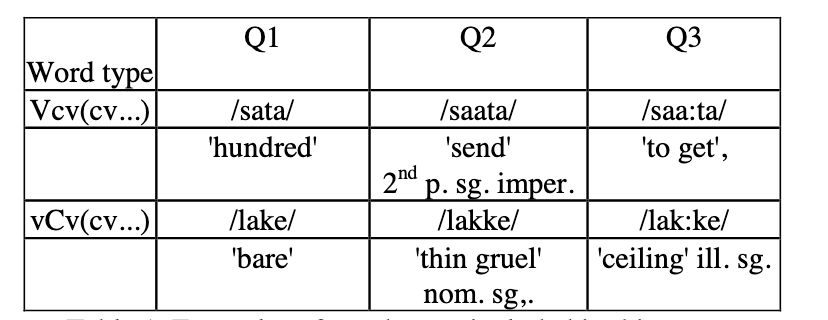
\includegraphics[width=200pt]{figures/Quantity.png}\\
%
% \caption{Ternary Quantity Contrast {\citep{krullFOOTISOCHRONYESTONIAN1999}}}
% \label{quant_cont}
% \end{center}
% \end{figure}
%
% \begin{table}[htb]
%\centering
%\begin{tabular}{lcc}
%\hline
%
%Q1 &		 sada 		& 	kabi  \\  
%	&	 {\it `hundred'} 	&	 {\it`hoof' }\\
%\hline
%Q2 &		saada 		&	kapi \\
%	&	 {\it`send' }		&	{\it`of the cupboard' }		\\
%\hline
%Q3 &		saada 	&	 kappi 	\\
%	&	{\it`recieve' }	&	{\it`into the cupboard' }	\\
%\hline
%\end{tabular}
%\label{qexamps}
%\caption{ternary syllable weight contrast}
%\end{table}
%
%
%\gll valge lauade vahele, \\
%white boards between \\
%\glt in between white boards, \\
% 
%Syllable weight or quantity also influences the otherwise predictable stress pattern. When a Q3 syllable is not in the first position, primary stress falls on it: this usually happens in the case of borrowed words. Otherwise, primary word stress is on the first syllable \citep{lehisteFunctionQuantityFinnish1965}. 
%  
%  \begin{table}[htb]
%\centering
%\begin{tabular}{lcr}
%\hline
% 	 Q1 – short 	&	ratio ~2/3 \\
%	 Q2 – long		& 	ratio ~3/2	\\
%	 Q3 – overlong	&	ratio ~2/1 	\\
%	 \hline
%\end{tabular}
%\label{stressick}
%\caption{c}
%\end{table}
%
%In the initial syllable of a word, syllable duration increases with syllable quantity, while the second syllable in the foot decreases as the first syllable's quantity increases. 
%
%It has been suggested, that the duration of the second vowel is a diagnostic of the quantity of the preceding syllable (duration ratios) \citep{lehisteFunctionQuantityFinnish1965, lehisteProsodicChangeProgress2003}. It has been suggested that this is due to the 
%a documented tendency for foot isochrony, wherein the total duration of disyllabic feet varies little in both spontaneous and read speech \citep{krullFOOTISOCHRONYESTONIAN1999, traunmullerEffectLocalSpeaking2003}resulting in the inverse relationship between the durations of the two syllables in a foot: the longer the first syllable, the shorter the second. More specifically: a second syllable that follow an overlong syllable will be realized shorter than a second syllable that follows a long syllable, with the longest second syllables following short (Q1) first syllables.  
%%\footnote{further discussion of perception of ternary quantity and duration ratios to put into prose \citep{foxDiscriminationDurationRatios1987,foxDiscriminationDurationRatios1989}}
%
%
%Duration ratios, but all proportionally 50\% differences. The ``long" second syllable of Q1 is shorter still than the ``short" second syllables of Q2 and Q3 feet. 
%\citep{lehiste1960segmental}
%\subsection{perception of word prosody}
%
%
%
%
%suggested analysis as types of foot accents rather than syllable degrees. 
%rising or falling f0 alone was insufficient to change the perceived category of all three weights.
%lengthening V2 of third quantity, but maintaining its reduction, did not suffice to change the perceived cat of A3 to A2: only when the tone contour also changed to rising did the nucleus duration facilitate. 
%reducing quality and shortening duration of nucleus V2 of an A2 alone also did not change perception to A3: only when falling tone added.
%\citep{eekSimplePerceptionExperiments1997}
%
%
%
%
%foot isochrony resulting in inversely proportional duration ratios of S1:S2 syllables, or more plainly that as S1 increases in quantity, S2 nucleus decreases. \citep{eekSimplePerceptionExperiments1997}
%
%Q3 vowels described as having especially large standard deviations \citep{eek1975}. 
%
%\section{Emphasis in Songs}
%\subsection{strong beats}
%
%\section{Template for {\it runosong}} 
%Kalevala and regilaul 
%\citep{sarv1998language}\\
%The singing of folksongs has long been an important part of the Estonian national heritage, and large scale community gathering to sing traditional {\it regilaul} songs is argued to have aided the preservation of Estonian cultural and linguistic heritage through long periods of occupation. \citep{bruggemannSingingOneselfNation2014}. The first documented song festival in Estonia was held in the seventeenth century \citep{ruutelTRADITIONALMUSICESTONIA2004}.
%
%Most descriptions of {\it regilaul} will describe it as ``non-western" folk music, though the definition of western escapes the author. It is perhaps the reduced use of tempered scale, although the songs have distinct tonal centers, and the melodies rise and fall in intervals from it.  The ``non-western" ness could equally be the lack of ``end-rhyming," a signature innovation in newer Estonian songs, as traditional {\it regilaul} rhymes little in favor of alliteration and parallelism. If you listen to them, though, even completely naive of the Estonian language, you will not mistake them for anything but a folksong, and a strictly structured one at that. 
%
%A song called {\it regilaul} is a type of Estonian folksong, found within the greater songwriting tradition of Balto-Finnic language family: variations on these songs are found in Finnish, Karelian, Votic, and Ingrian traditions \citep{tormisKalevalaEstonianPerspective1985}. 
%
%Collectively, songs in this tradition are often referred to as ``runosongs" or ``runic songs." 
%
%These runic songs are set in what scholars refer to as The ``Kalevala" metre, named for the title of the epic poem in Finnish; Estonia's own version is called ``Kalevipoeg" {\it Kalev's son}. 
%
%In the story, Kalevipoeg is a giant with a hedgehog for a companion. 
%
%The poem contains songs, too: a consistent theme across these poems and Estonian folklore generally has protagonists requesting song lyrics and incantations from deities, often in pursuit of skill in dance or music. 
%
%In studies of metre, a trochee is a disyllabic sequence with a strong first syllable and a weak second. In {\it regilaul} songs, the strong position of a two note sequence is called ``ictus," and the weak position is called ``off-ictus"
%
% The basic template of the Kalevala metre is four trochees per line, for a total of eight syllables. There are of course variations, but the basic invariant {\it regilaul} verse line will contain eight beats evenly divided into a single measure: in a 4/4 song, each of the eight syllables corresponds with one eighth note. In this case each eighth note will correspond to one syllable in the text, the constituent henceforth referred to as the ``syllable-note" \citep{ruutelResultsComputerizedComparative1999}. The late composer and {\it regilaul} revitalist Veljo Tormis referred to the runic songs as ``singable songs" \citep{tormisProblemsThatRegilaul2007}. 
% 
% ``collaborative outcomes" 
% in regilaul, the musical rhythm is directly connected to the verse structure \citep{orasMusicalManifestationsTextual2010}
% 
% Due to the strict metrical parametres of the form, any runosong text can be sung to any runosong melody. An example of this in English: one can sing {\it Amazing Grace} to the tune of {\it House of the Rising Sun}, and vice a versa.\footnote{Also try TLC's ``Scrubs" exchanged with America's ``Horse With No Name"}. 
%\begin{figure}[htb]
%\begin{center}
%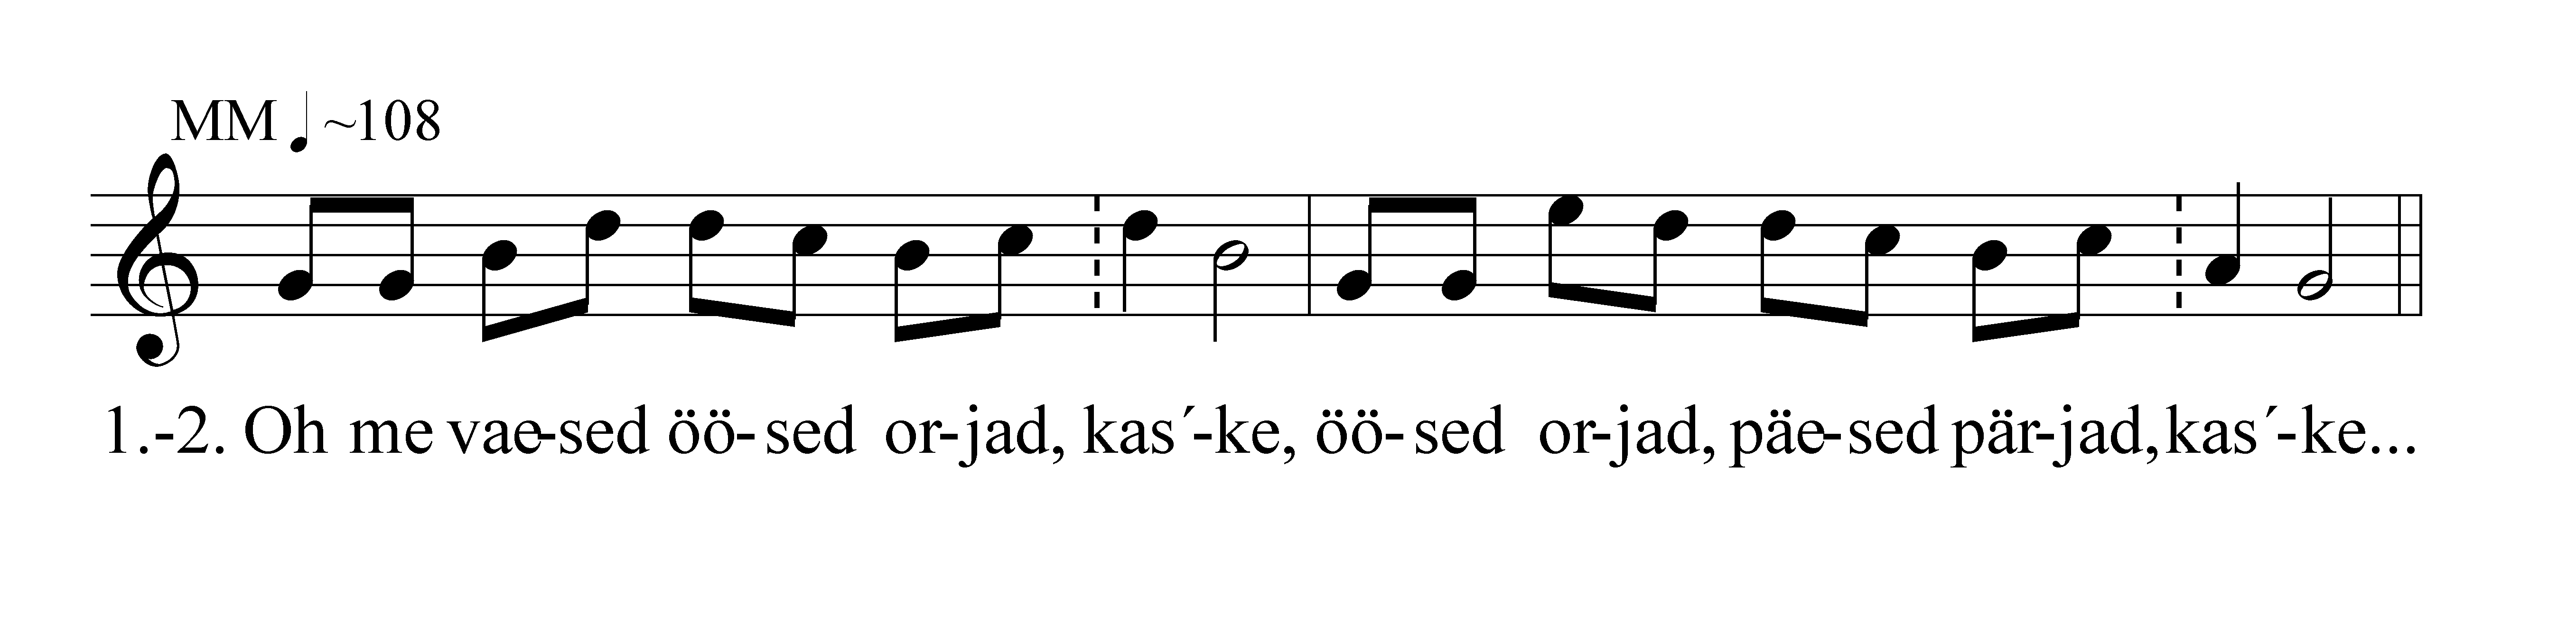
\includegraphics[width=300pt]{figures/069.png}
%\caption{Öised orjad, performed by Liisu Orik}
%\label{song69}
%\end{center}
%\end{figure}
%
%In \ref{song69}, we see the musical notation of a typical {\it regilaul} verse: eight notes evenly divided into a measure (eight eighth notes) and corresponding one syllable per eighth note as indicated by the text. The refrain {\it kas`-ke}, which is repeated after every verse line, is part of a separate musical phrase, though it is not a full measure on its own (it contains only three beats). This is indicated by the dashed line following the first measure of the verse. The solid bar after the {\it kas`-ke} refrain indicates the onset of a new ``regular" measure, another {\it regilaul} verse line of eight syllables evenly divided into eighth notes in the measure. 
%
%\begin{figure}[htb]
%\begin{center}
%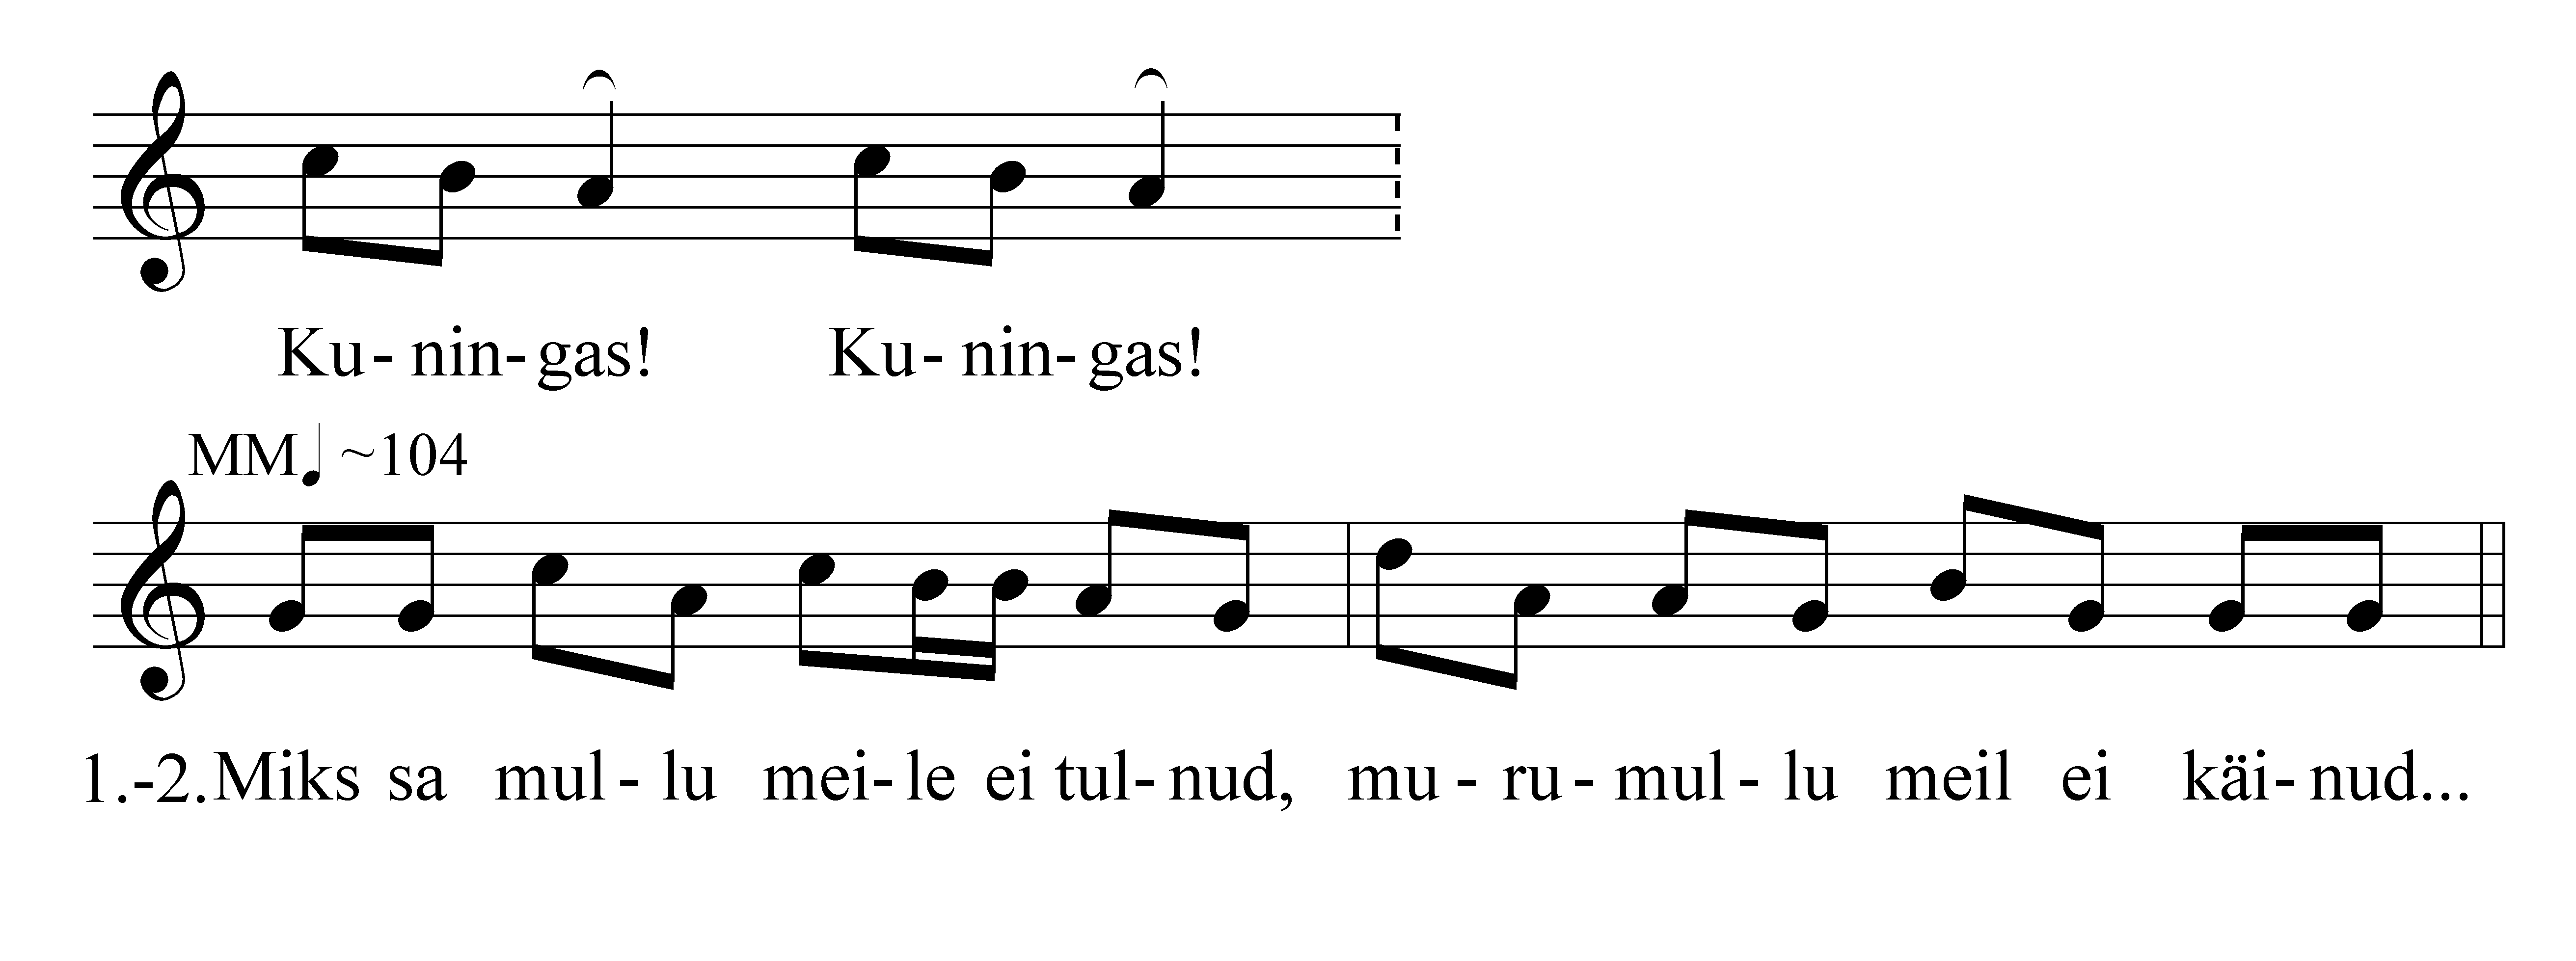
\includegraphics[width=300pt]{figures/094.png}
%\caption{`The King Game" as performed by Liisa Kümmel on track 94 of the anthology}
%\label{kinggame}
%\end{center}
%\end{figure}
%
%In \ref{kinggame} we see an example of extra syllables fit into the Kalevala metre. The first measure in the figure is another refrain. Looking at the verse annotation, we see that there are in fact nine syllables instead of the requisite eight. The measure accomodates the extra syllable by dividing one of the eighth notes into two sixteenths. Thus, the one to one ratio of syllable to note remains, but only seven of the syllable-notes are annotated as isochronous. 
%
%Only those syllable-notes which are in evenly divided verse measures are the subject of this study. Non-verse notes, such as those in refrains, as well as notes in verses that occupy a different categorical duration than other notes in its measure are not included. 
%
%
%The composer Veljo Tormis refers to folksongs in this tradition as ``singable song," 
%
%shared structure of other Finno-Ugric language family, i.e., %
%%
%the singable song 
%
%
% ancient epic tale shared by many members of the Finno-Ugric language family
% 
% The common folklore of Finno Ugric language family: Kalavala in Finland, Kalevipoeg (Kalev's son) in Estonia. Kalev is a giant. His companion is a hedgehog.  
% many stories involve a character seeking incantations (song lyrics) to acquire some skill
% 
%
%
%\subsection{Previous phonetic studies of Estonian metrics and {\it regilaul}}
%
% \citep{palmerLinguisticProsodyMusical1992} hypothesize that prosodic stress and musical metre align in song, but their measurements were only of English vocalists and ``western" music. 
%English vocalists were asked to perform songs in which stressed syllables aligned or clashed with the musical meter, finding relative increases in syllable duration in at both word-level and song-level positions of prominence \citep{palmerLinguisticProsodyMusical1992}, suggesting that the two systems contribute separately but use similar organizational properties.
%
%Ilse Lehiste analyzed spoken poems in Estonian and Finnish, examining the differences in quantity relations under metrical subjugation and found that in strict metrical forms (i.e., the Kalevala metre), the absolute durations of Q2 and Q3 metrical feet lost their contrast, but retained the approximate ratio of durations between the first and second syllable. In freer verse, the differences in absolute durations remained, suggesting that the duration ration between Q2 and Q3 is an important cue for contrast, especially in the contexts of temporal demands of an imposed paralinguistic metre. 
%\citep{lehistePhoneticsMetrics1992} Later, in collaboration with Jaan Ross, three papers examined the phonetics of metrics in old Estonian {\it regilaul} folksongs. The first (Funeral laments study )\citep{rossLostProsodicOppositions1994}, finding that duration was best predicted by metrical position and not syllable quantity. 
%
%
%
%
%They later found that duration was a better predictor of ictus  than of word stress: stressed syllables in off-ictus lost their durational contrast with unstressed syllables.  \citep{rossTradeoffQuantityStress1996} 
%
%In \citep{rossTimingEstonianFolk1998} Ross and Lehiste measure syllable duration ratios for Q1 initial syllables of disyllabic feet: falling in ictus position and falling in off-ctus position. They found that the duration ratios of Q1 syllables in ictus were greater than those in off-ictus. In ictus position, Q1 syllables were roughly the same length as each other, while those in off-ictus were shortened. They conclude the duration cue for contrastive stress is subordinated to the song. 
%This paper aims to extend the findings of the aforementioned studies \citep{lehistePhoneticsMetrics1992, rossLostProsodicOppositions1994,rossTradeoffQuantityStress1996,rossTimingEstonianFolk1998} by annotating a larger corpus of {\it regilaul}, to compare conflicts of song stress (ictus) and word stress 
%and investigate whether syllable quantity contrast is preserved in song. Vowel duration is an acoustic correlate of both syllable stress and quantity, and so I measure vowel duration in the context of performed {\it regilaul} songs. 
%
%Vowel duration, if subordinated to the metre of the song, would confirm Ross \& Lehiste's results \citep{rossLostProsodicOppositions1994, rossTimingEstonianFolk1998, rossTradeoffQuantityStress1996}. 
%
%If this question has already been investigated, what motivates the author to pursue it further? First, the aforementioned studies were limited in sample size: each one examined only one word-level interaction with song-level prominence, when both are well documented to influence duration in spoken Estonian, and with each other. Thus, the present study examines all three predictors of prominence: song ictus, word stress, and syllable quantity. I also exponentially increase the {\it n} of trials for increased robustness, and then analyze the dataset using Bayesian modeling techniques to capture the nuanced covariance of the three predictor categories. In addition to replicating duration measurements undertaken in earlier studies, I also introduce vowel space as a potential predictor for word-level prominence. 
%
%more recently, text setting in regilaul
%\citep{orasMusicalManifestationsTextual2010}
%
%
%
%
%A good deal of literature has been devoted to the classification of languages by typological rhythms: in particular, ``stress-timed," ``syllable-timed," and ``morae-timed" systems have been proposed. An extremely reductionist description of these typologies would assert a relative isochrony of the named constituent. That is, a language that has been described as ``stress-timed" is said to be "timed" according to, and having relative isochrony of stressed syllables. Likewise, a syllable-timed language would be described as having syllabic isochrony, and so on. Many of these notions are based on the intuitions of native speakers, however, supporting phonetic data is limited  \citep{kohlerRhythmSpeechLanguage2009}. 
%%add later!!: (Bertinetto 1989) (Kohler 2009a, b). 
%More recently, alternate rhythmic metrics have entered the discussion in support of timing classes: i.e., Pairwise Variability Index (PVI), normalized Pairwise Variability Index (nPVI), both of which use the relationship of durations of adjacent syllables to describe their timing classes.\citep{arvanitiRhythmClassesSpeech2012}. English, for example, has higher syllable PVI (Pairwise Variability Index) than Estonian, due to English's drastic reduction of weak syllables, and the presence of prominent short syllables ( i.e., syllable durations in English are more variable than in Estonian)\citep{asuEstonianEnglishRhythm2006}. 
%
%
% 
% 
%\begin{itemize}
%\item is stress or ictus a better predictor of vowel duration?
%\item is the ternary syllable quantity contrast preserved in {\it regilaul} songs?
%\end{itemize} 
%
%\subsection{Design of the Study}
%
%Measurements:
%
%vowel duration
%
%vowel dispersion
%
%stressed syllable less reduced, more intelligible, 
%
%Fine-grained acoustic-phonetic cues to stress (cross-linguistic) 
%\citep{lindblom1990,moonInteractionDurationContext1994, de1995supraglottal, bradlowIntelligibilityNormalSpeech1996,smiljanicProductionPerceptionClear2005} \\
%\subsection{On foot isochrony and duration ratios} 
%
%However, in both cases, the presence of foot isochrony and consistent duration ratios across these three types of feet would not indicate that the foot is the domain of the contrast, nor that the ratio itself is the measurement of importance. Instead, these two findings point to the level of contrast between Q1, Q2, and Q3 syllables at the level of the syllable, and the resulting fluctuations in ratios of first and second syllables as inevitable consequences of preserving the contrast in initial position. 
%
%Another consideration is that the three quantities are not restricted to length contrasts of identical segments, in the case of the geminates seen in minimal triads, but also can be comprised of diphthongs and complex codas {\it in addition} to geminates. 
%, i.e., ui: (diphthong ending in long V), diphthong complex coda geminate consonant, etc. \\ 
%
%
%contain more phoneme segments. The minimal triads illustrate the segmental length contrasts that provide evidence for the three weights of syllables in primary stress position, but they do not adequately convey that the different quantities are not simply different lengths of segments, but that with an increase syllable quantity comes an increase in the quantity of segments contained within that constituent. To illustrate this, the table in \ref{} contains representations of available segment combinations in each syllable, and examples of Estonian near-minimal triads in disyllabic words. 
%

%\chapter{Handout}


The rhythmic organization of song integrates the prosodic structure of the language with musical rhythmic principles \citep{palmerLinguisticProsodyMusical1992}. 

Duration can be a phonetic correlate of stress, and it can also be independently contrastive at the segmental level \citep{lehistePhoneticsMetrics1992}. 


%Whether there is a correlation between poetic metre and the prosodic structure of a language.

%A trochee is a strong, stressed syllable followed by a short(er), weak syllable. 




\citep{lehistePhoneticsMetrics1992} investigated the actual phonetic realization of different metres in different languages, finding evidence for one language's trochee, for example, to be realized in a way that is systematically different from another language's trochee. 

Ross found vowel reduction in certain notes, but they were all unstressed, off-ictus for that song\citep{rossFormants90}.


The role of primary stress in Estonian is described by Ilse Lehiste as {\it identificational} rather than contrastive \citep{lehistePhoneticsMetrics1992}. In other words, there are no stress minimal pairs at the lexical level, so the prominence cue is to indicate the onset of a new word. This is sometimes also called {\it demarcative} stress.



Three proposed levels of stress: primary stress, unstress, and secondary stress. \citep{lippusAcousticStudyEstonian2014a}

Primary lexical stress in native Estonian words is fixed, falling on word-initial syllables. 
\cite{eekmeisterUralica98}
\begin{exe}
\ex \gll laul-da \\
	{[ˈlɑuːl.dɑ]} \\
	sing-\Tr{} 
	\glt	`singing'
\ex 	ööbik \\
	{[ˈøː.pikː]} \\
	nightingale.\Nom{} 
	\glt`nightingale'
\end{exe}

Estonian has three syllable weights, also called degrees or quantities, that are contrastive in primary stress position. The first degree or Q1 is described as short, 
%In \ref{quant_cont}, we see two minimal pairs illustrating this contrast. 

This ternary contrast has long been the subject of debate in the phonological literature of metrics: Q3 syllables have been analyzed both as a monosyllabic foot \citep{princeMetricalTheoryEstonian1980} and as a trimoraic syllable \citep{hayesCompensatoryLengtheningMoraic1989, kuznetsovaEstonianWordProsody2018,prillopMoraeEstonianReply2020}. 


 \begin{table}[htb]
\centering
\begin{tabular}{lcc}
\hline

Q1 &		 sada 		& 	kabi  \\  
	&	 {\it `hundred'} 	&	 {\it`hoof' }\\
\hline
Q2 &		saada 		&	kapi \\
	&	 {\it`send' }		&	{\it`of the cupboard' }		\\
\hline
Q3 &		saada 	&	 kappi 	\\
	&	{\it`recieve' }	&	{\it`into the cupboard' }	\\
\hline
\end{tabular}
\label{qexamps}
\caption{ternary syllable weight contrast}
\end{table}

%\chapter{Regilaul: Estonia's {\it runosong} tradition}
\index{Runsong and the Kalevala}@\emph{Runosong and the Kalevala}



\begin{figure}[htbp]
\begin{center}
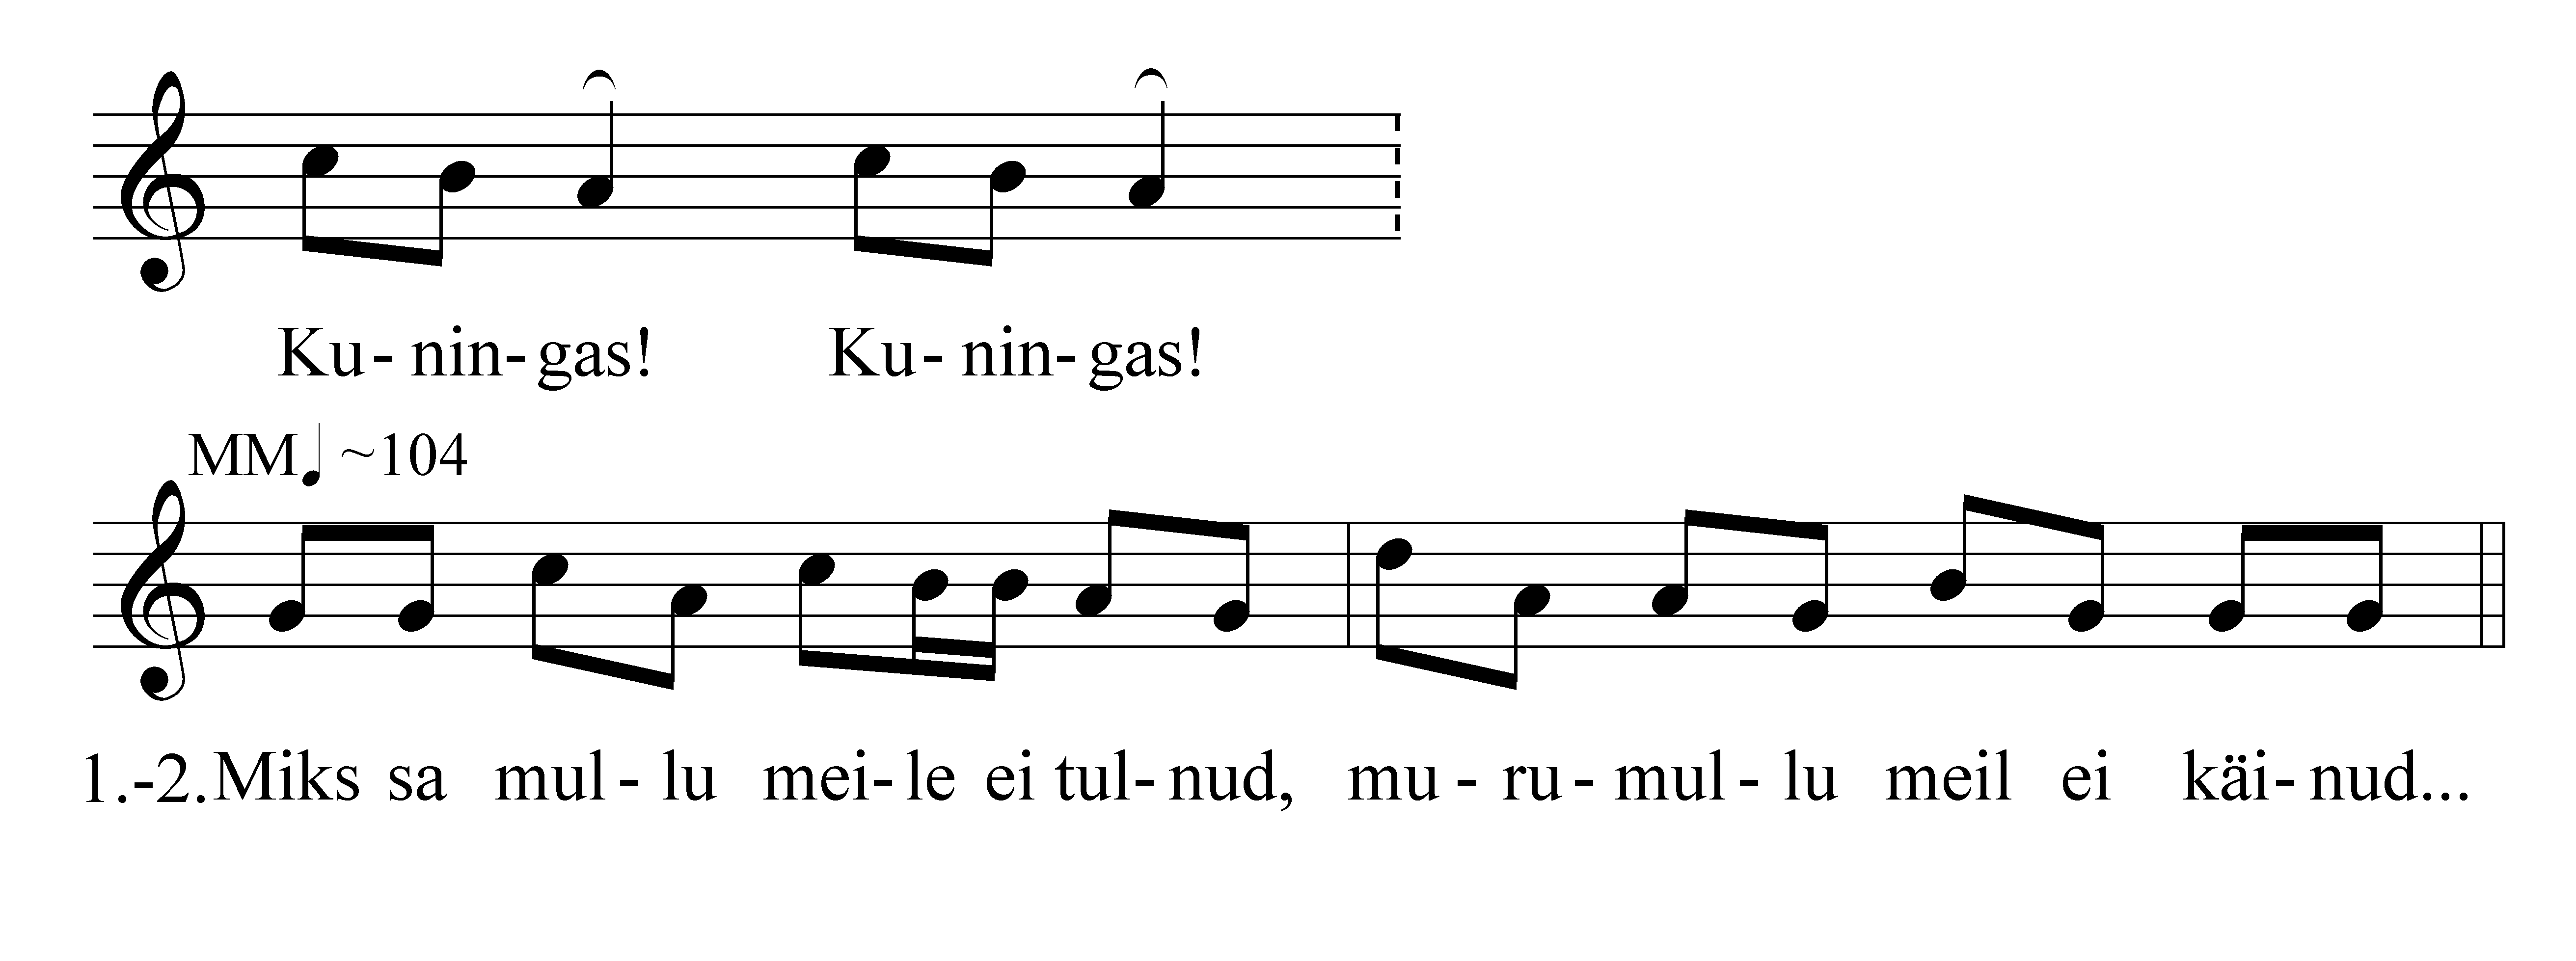
\includegraphics[width=300pt]{figures/094.png}
\caption{music notation of ``The King Game" as performed by Liisa Kümmel}
\label{The King Game}
\end{center}
\end{figure}

\section{The Runic Song Tradition} 


A given {\it regilaul} verse line contains eight beats, generally evenly divided into a single measure so that each of the eight syllables corresponds with one eighth note. The ictus position of a song's line is thus determinable by counting every other beat as ictus, starting with the first.

The first song festival in Estonia held in \cite{ruutelTRADITIONALMUSICESTONIA2004}. 


One runic invariant is that the tonal center is placed on ``the both syntactically stable 


dominating pitch value of the most stable syntactical positions of a given melody's typological group


the syllable-note is the basic unit of the melody-line. Thus syllables take up the space of the note in their position of the melody as prescribed. 


Melodic accents coincide with the stressed syllables, the pitch resolves as the phrase resulves. Said to be a musical abstraction of the natural prosodic intonation of the 8 syllable (spoken) runoverse. 
\cite{ruutelResultsComputerizedComparative1999} 

%
%\section{The singing giant: a common folklore epic} 
%Estonian, Finnish, Karelian, Ingrian runic songs
%
%whether it be Finnish, Estonian, Karelian, Votic, Ingrian and to same extent even Livonian an Veps)
%
%
%the singable song \cite{tormisKalevalaEstonianPerspective1985}
%
%
% ancient epic tale shared by many members of the Finno-Ugric language family
% 
% The common folklore of Finno Ugric language family: Kalavala in Finland, Kalevipoeg (Kalev's son) in Estonia. Kalev is a giant. His companion is a hedgehog.  
% many stories involve a character seeking incantations (song lyrics) to acquire some skill
% 
 
 \cite{tormisProblemsThatRegilaul2007}
\section{regilaul in prosodic contexts}



\cite{lehistePhoneticsMetrics1992}








 
 
\section{Previous Studies with regilaul}

\begin{figure}[htbp]
\begin{center}
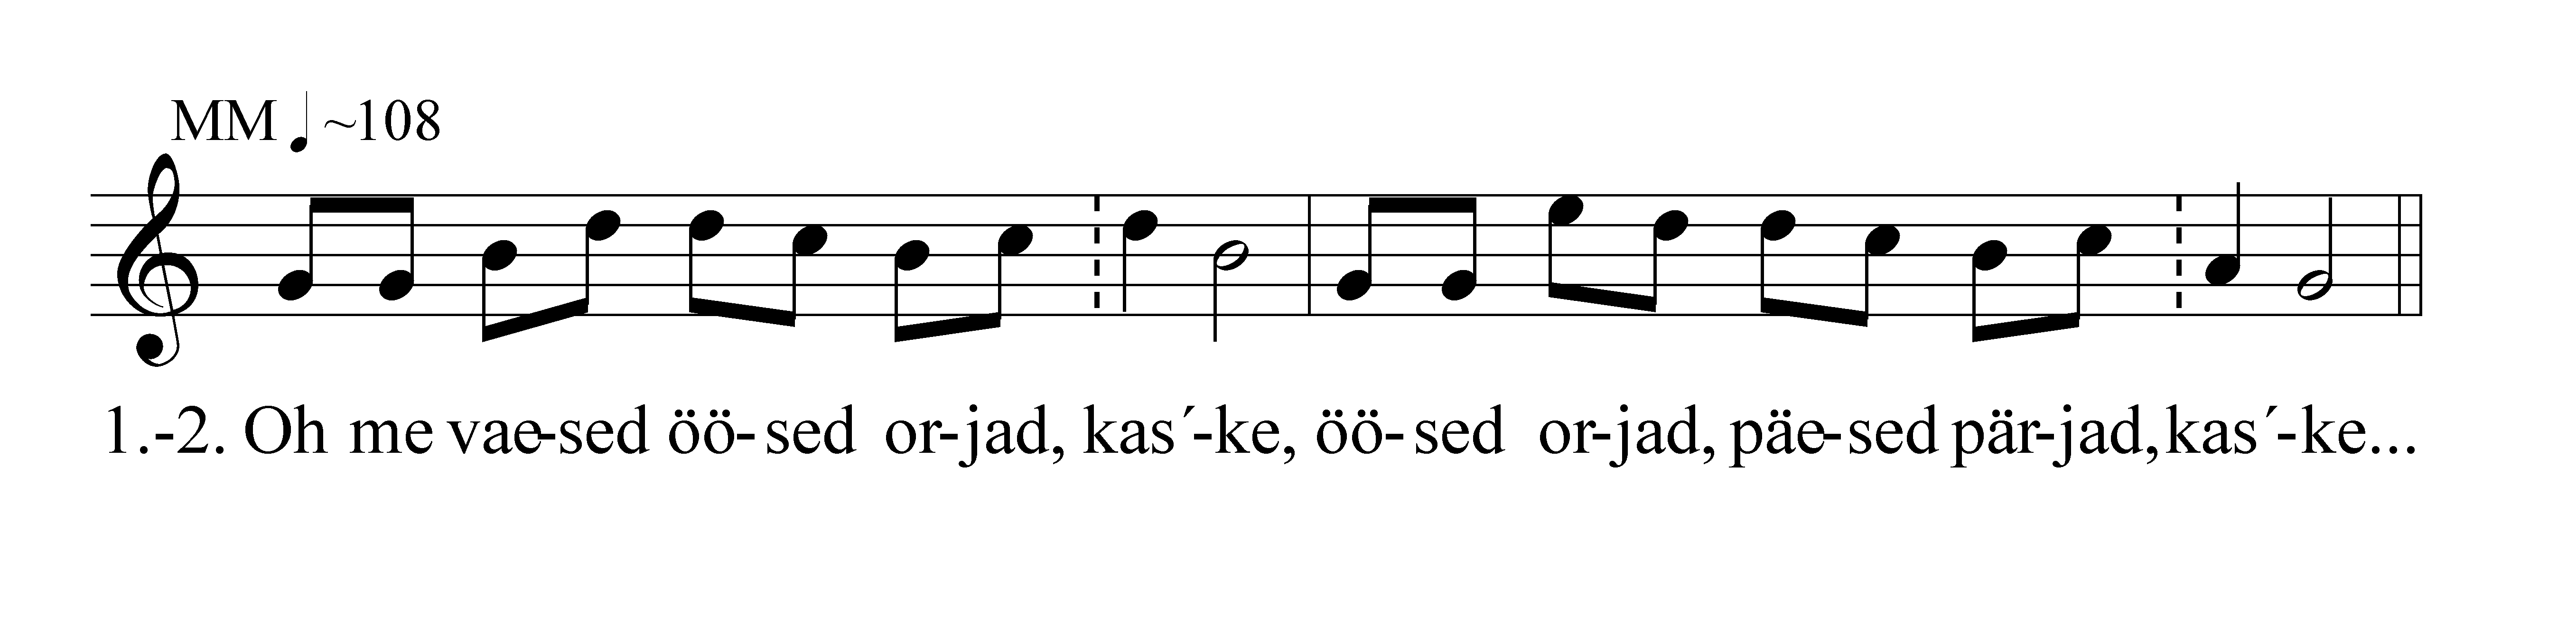
\includegraphics[width=300pt]{figures/069.png}
\caption{default}
\label{default}
\end{center}
\end{figure}

\cite{rossStudyTimingEstonian1989,rossLostProsodicOppositions1994,rossTradeoffQuantityStress1996,sargDoesMelodicAccent2006, sargMelodicAccentEstonian2007,orasMusicalManifestationsTextual2011}

%\chapter{Making the Bibliography with BiB\TeX{}}\label{c:bib}
\index{Making the Bibliography with BiBTeX%
@\emph{Making the Bibliography with BiB\TeX{}}}%

BiB\TeX{} 
\index{BiBTeX@BiB\TeX{}}%
allows one to generate automatically the bibliography 
from a database of bibliographic 
items. You need to do the following:

\begin{enumerate}
\item Create the bibliographic database, 
\index{bibliographic database}%
which is a file whose name ends in \texttt{.bib}. 
\index{.bib@\texttt{.bib}}%
Let us call it \texttt{diss.bib}. Entries in this file are like this:
\begin{verbatim}
@BOOK{knuth:tb,
  author = "Donald K. Knuth",
  title = "The \TeXbook",
  publisher = "Addison-Wesley",
  year = "1984",
}
@TECHREPORT{poorten:sp,
  author = "Alf~J.~van der Poorten",
  title = "Some problems of recurrent interest",
  institution = "School of Mathematics and Physics,
                 Macquarie University",
  address = "North Ryde, Australia 2113",
  number = "81-0037",
  month = "August",
  year = "1981",
}
@ARTICLE{erdos:oap,
 author = "Paul Erd{\"o}s and Paul Turan",
 title = "On a problem in the theory of uniform 
          distribution, {I}", 
 journal = "Indag. Math.",
 volume = "10",
 year = "1948",
 pages = "370--378",
}
\end{verbatim}

\item Include a \cn{bibliographystyle} 
\index{commands!bibliographystyle@\cn{bibliographystyle}}%
command in your \LaTeX{} file, say 

\cn{bibliographystyle\{plain\}} 
and a \cn{bibliography} 
\index{commands!bibliography@\cn{bibliography}}%
command to load the bibliography, 
in this case \cn{bibliography\{diss\}}, at the point of your 
document where the bibliography should be inserted. 

The document at this point will look like this:
\begin{verbatim}
\bibliographystyle{plain}
\bibliography{diss}
\end{verbatim}

\item Run \LaTeX{} on your main file, say \texttt{foo.tex}: 
\texttt{latex foo}. This generates an auxiliary file 
\texttt{foo.aux} with a list of \cn{cite} 
\index{commands!cite@\cn{cite}}
references.

\item Run BiB\TeX{} on your file: \texttt{bibtex foo}. 
BiB\TeX{} reads the auxiliary file, looks up the 
bibliographic database (\texttt{diss.bib}), 
and writes a \texttt{.bbl} 
\index{.bbl@\texttt{.bbl}}%
file with the bibliographic information formated according to
the bibliographic style file (\texttt{.bst}, 
\index{.bst@\texttt{.bst}}%
say \texttt{plain.bst}) 
\index{plain.bst@\texttt{plain.bst}}%
specified.  Messages about resources used and error messages
are written to a \texttt{.blg} 
\index{.blg@\texttt{.blg}}%
file (in the case of this template, disstemplate.blg).

\item Run \LaTeX{} again: \texttt{latex foo}, which now 
reads the \texttt{.bbl} 
\index{.bbl@\texttt{.bbl}}%
reference file.

\item Run \LaTeX{} for a third time: \texttt{latex foo}, 
resolving all references.

\end{enumerate}

This includes all bibliographic items that have been cited 
in the document with a \cn{cite} 
\index{commands!cite@\cn{cite}}%
command. In order to include non cited items in the bibliography,
use the command \cn{nocite}. For example, \cn{nocite\{knuth:tb\}}
anywhere in the document (after \cn{begin\{document\}}) includes 
in the bibliography the item with label \texttt{knuth:tb}. 
In order to include \emph{all} items of the bibliographic 
database, use the command \cn{nocite\{*\}}.
\index{commands!nocite@\cn{nocite}}%

%
%\chapter{Making Tables and Including Figures}
\index{Making Tables and Including Figures@\emph{Making Tables
	and Including Figures}}%

The \emph{tabular} 
\index{commands!environments!tabular}%
environment allows us to create complex 
tables and figures, and draw boundaries around and within it.
The following example illustrates this:

\begin{table}[h]
\begin{center}
\caption{An example of a table.}
\vskip 10pt
\begin{tabular}{|ll|l|ll|l|lll|}
\cline{1-2} \cline{4-5} \cline{7-9}
\multicolumn{2}{|c|} {\textsl{Gegenwart}} & &
\multicolumn{2}{|c|} {\textsl{Imperfekt}} & &
\multicolumn{3}{|c|} {\textsl{Perfekt}} \\
\cline{1-2} \cline{4-5} \cline{7-9}
ich & bin  & & ich & war   & & ich & bin  & gewesen \\
du  & bist & & du  & warst & & du  & bist & gewesen \\
er  &      & & er  &       & & er  &      &         \\
sie & ist  & & sie & wart  & & sie & ist  & gewesen \\
es  &      & & es  &       & & es  &      &         \\
\cline{1-2} \cline{4-5} \cline{7-9}
wir & sind & & wir & waren & & wir & sind & gewesen \\
ihr & seid & & ihr & wart  & & ihr & seid & gewesen \\
sie & sind & & sie & waren & & sie & sind & gewesen \\
\cline{1-2} \cline{4-5} \cline{7-9}
Sie & sind & & Sie & waren & & Sie & sind & gewesen \\
\cline{1-2} \cline{4-5} \cline{7-9}
\end{tabular} \\[10pt]
Note: The assistance of Herr Professor Lothar Frommhold \\
in generating this table of German declensions \\
is gratefully acknowledged.
\vskip -20pt
\end{center}
\end{table}
\index{commands!environments!table}%

This table was created with the following sequence 
of commands:
\begin{verbatim}
\begin{table}[h]
\begin{center}
\caption{An example of a table.}
\vskip 10pt
\begin{tabular}{|ll|l|ll|l|lll|}
\cline{1-2} \cline{4-5} \cline{7-9}
\multicolumn{2}{|c|} {\textsl{Gegenwart}} & &
\multicolumn{2}{|c|} {\textsl{Imperfekt}} & &
\multicolumn{3}{|c|} {\textsl{Perfekt}} \\
\cline{1-2} \cline{4-5} \cline{7-9}
ich & bin  & & ich & war   & & ich & bin  & gewesen \\
du  & bist & & du  & warst & & du  & bist & gewesen \\
er  &      & & er  &       & & er  &      &         \\
sie & ist  & & sie & wart  & & sie & ist  & gewesen \\
es  &      & & es  &       & & es  &      &         \\
\cline{1-2} \cline{4-5} \cline{7-9}
wir & sind & & wir & waren & & wir & sind & gewesen \\
ihr & seid & & ihr & wart  & & ihr & seid & gewesen \\
sie & sind & & sie & waren & & sie & sind & gewesen \\
\cline{1-2} \cline{4-5} \cline{7-9}
Sie & sind & & Sie & waren & & Sie & sind & gewesen \\
\cline{1-2} \cline{4-5} \cline{7-9}
\end{tabular} \\[10pt]
Note: The assistance of Herr Professor Lothar Frommhold \\
in generating this table of German declensions \\
is gratefully acknowledged.
\vskip -20pt
\end{center}
\end{table}
\index{commands!environments!table}%
\end{verbatim}

The argument \texttt{h} indicates the position for the 
table, in this case ``here if possible''. Other values
of this argument are:
\texttt{t} (top of the page),
\texttt{b} (bottom of the page),
\texttt{p} (on the page of floats) and 
\texttt{H} (HERE! - requires using the package float.sty.
Note: When this option is used, LaTeX ignores all of its formatting
rules and does what you say, putting the entire float exactly where
it is defined. Check your output to make sure it is what you want!
If you are having trouble with LaTeX wanting to put a figure that's
larger than roughly half-a-page, as well as all of the figures
following it, at the end of a chapter, try using the command
\cn{clearpage} immediately following the large figure --- and maybe
a \cn{newpage} later.)
It is possible to combine several arguments, such as
\texttt{ht} (``here if possible, otherwise on top of
the page''). The default is \texttt{tbp}.

Figure \ref{f:ex} is a typical example of inclusion of a 
figure contained in an encapsulated PostScript file. 
\index{PostScript}%
\index{encapsulated PostScript}%
In order to use it, it is necessary to include the 
command \cn{usepackage\{psfig\}} 
\index{psfig}%
at the beginning of the document.

\begin{figure}[htb] % Imported eps example.
\begin{center}
\ 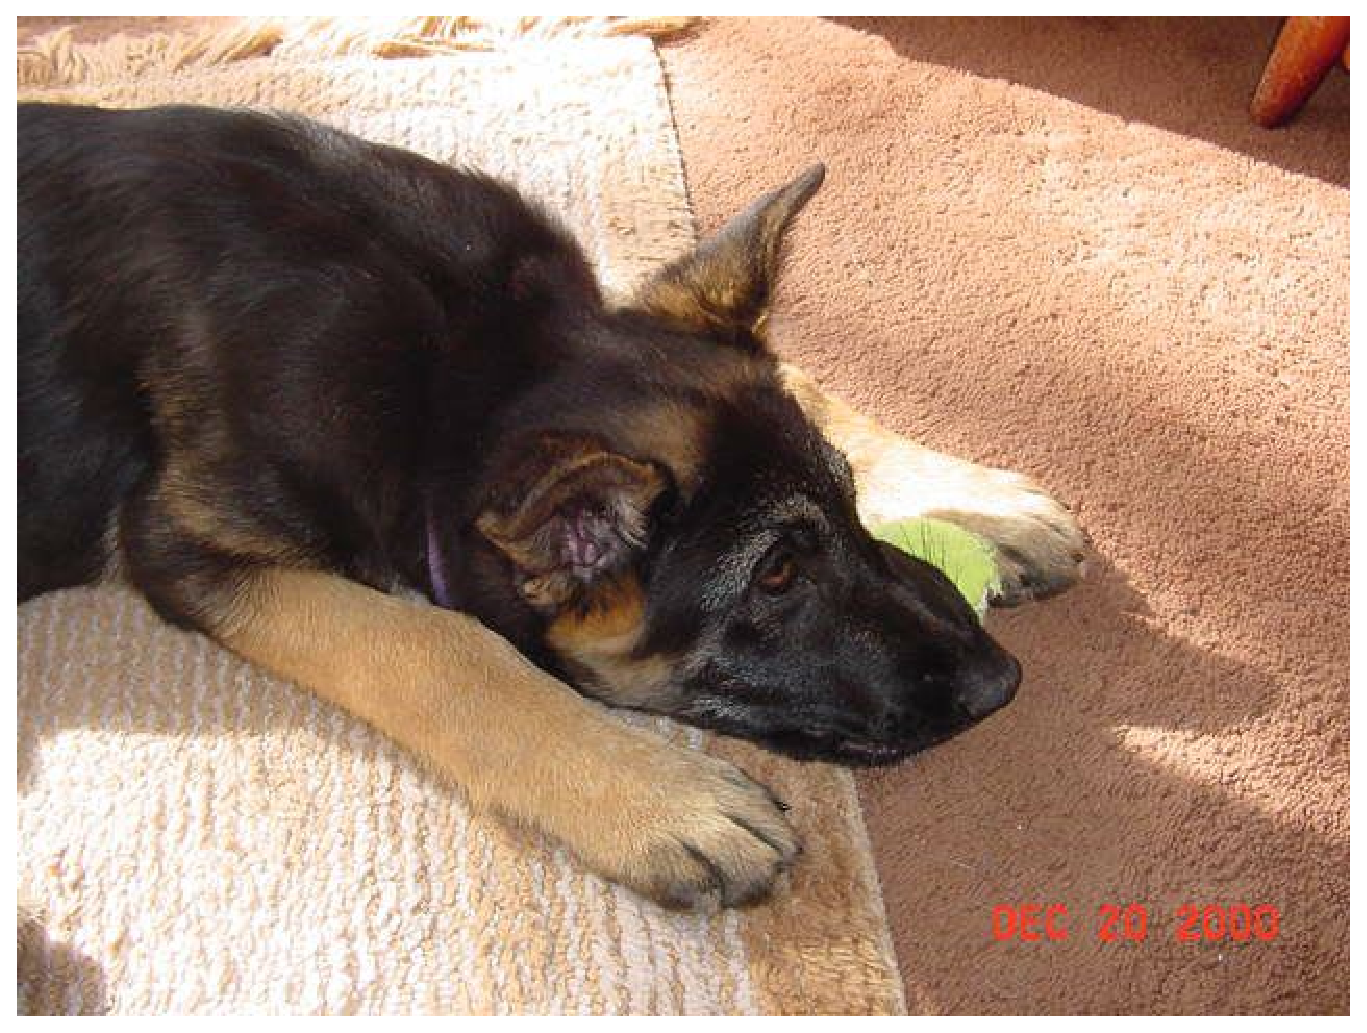
\psfig{file=pup-on-rug.eps,height=1.5in,width=2.0in}
\caption{An example of an imported eps file.}
\label{f:ex}
\end{center}
\end{figure}
\index{commands!environments!figure}%
You can see the commands that generated this
figure in the source file. Look for the line
\cn{begin\{figure\}[htb] \% Imported eps example. }

The command that imports the file is \cn{psfig}, and it also 
controls its size (\texttt{height} and \texttt{width}), and 
can rotate the figure (\texttt{angle}).

Figures can also be drawn by using \LaTeX{} commands. 
Figure \ref{f:circuit} is an example 
(taken from \cite{gms:tlc}).

\begin{figure}[htb] % Picture example.
\begin{center}
   \setlength{\unitlength}{4mm}
   \begin{picture}(12,10)(-2,0)
      \linethickness{0.4pt}
      \qbezier(2.00,6.00)(7.00,6.00)(9.00,3.00)
      \qbezier(2.00,0.00)(7.00,0.00)(9.00,3.00)
      \qbezier(2.00,6.00)(4.00,3.00)(2.00,0.00)
      \qbezier(1.00,6.00)(3.00,3.00)(1.00,0.00)
      \put(9.75,3.00){\circle{1.50}}
      \put(10.50,3.00){\line(1,0){1.50}}
      \put(0.00,5.00){\line(1,0){1.50}}
      \put(0.00,1.00){\line(1,0){1.50}}
   \end{picture}
\caption{An example of a picture}
\label{f:circuit}
\end{center}
\end{figure}
\index{picture}%

The commands that generated this
picture are in the source file following the line
\cn{begin\{figure\}[htb] \% Picture example.  }

The commands used have rather obvious meanings. In particular, 
the command \cn{qbezier} 
\index{commands!qbezier@\cn{qbezier}}%
draws a quadratic Bezier curve, 
defined by its two ending points, and a third point (whose 
coordinates are in the middle) that is used as control point. 
Figure \ref{f:qb} illustrates the effect of the control point:

%\begin{figure}[htb] % Bezier curves example.
\begin{figure}[h] % Bezier curves example.
\begin{center}
   \setlength{\unitlength}{.8mm}
   \begin{picture}(55,55)(-15,0)
      \linethickness{1pt}
      \qbezier(0,0)(-10,30)(50,30)
      \qbezier(0,0)(20,50)(50,30)
      \thinlines
      \put(0,0){\line(-1,3){10}}
      \put(50,30){\line(-1,0){60}}
      \put(0,0){\line(2,5){20}}
      \put(50,30){\line(-3,2){30}}
      \put(0,0){\circle*{1}}
      \put(0,-1){\makebox(0,0)[t]{$A_{0,0}$}}
      \put(-10,30){\circle*{1}}
      \put(-10,31){\makebox(0,0)[b]{$B_{10,30}$}}
      \put(50,30){\circle*{1}}
      \put(58,29){\makebox(0,0)[b]{$C_{50,30}$}}
      \put(20,50){\circle*{1}}
      \put(20,51){\makebox(0,0)[b]{$D_{20,50}$}}
   \end{picture}
\caption{Bezier curves}
\label{f:qb}
\end{center}
\end{figure}
\index{Bezier curves}%


This figure has been generated with the following commands:
\begin{verbatim}
\begin{figure}[htb] % Bezier curves example.
\begin{center}
   \setlength{\unitlength}{.8mm}
   \begin{picture}(55,55)(-15,0)
      \linethickness{1pt}
      \qbezier(0,0)(-10,30)(50,30)
      \qbezier(0,0)(20,50)(50,30)
      \thinlines
      \put(0,0){\line(-1,3){10}}
      \put(50,30){\line(-1,0){60}}
      \put(0,0){\line(2,5){20}}
      \put(50,30){\line(-3,2){30}}
      \put(0,0){\circle*{1}}
      \put(0,-1){\makebox(0,0)[t]{$A_{0,0}$}}
      \put(-10,30){\circle*{1}}
      \put(-10,31){\makebox(0,0)[b]{$B_{10,30}$}}
      \put(50,30){\circle*{1}}
      \put(58,29){\makebox(0,0)[b]{$C_{50,30}$}}
      \put(20,50){\circle*{1}}
      \put(20,51){\makebox(0,0)[b]{$D_{20,50}$}}
   \end{picture}
\caption{Bezier curves}
\label{f:qb}
\end{center}
\end{figure}
\end{verbatim}


%
%\chapter{An Example of Mathematical Writing}
\index{An Example of Mathematical Writing%
@\emph{An Example of Mathematical Writing}}%

\section{Generalized Fatou's Lemma}
\index{Generalized Fatou's Lemma%
@\emph{Generalized Fatou's Lemma}}%

Here we show an application of the following lemma:

\begin{lem}[Generalized Fatou's Lemma] \label{l:fatou}

Let $A$ be a Dedekind ring and $F$ a rational series 
in $A[[X]]$, i.e., $F = p/q$ for some 
$p, q \in A[X]$. Then there exist two polynomials 
$P, Q \in A[X]$ such that $F = P/Q$, 
where $P$ and $Q$ are relatively prime and 
$Q(0) = 1$.

\end{lem}

\proof
See \cite{bertin:psn}, p.~15, theorem~1.3.
\endproof

\begin{thm} \label{l:req}
Let $\{c_n\}_{n=-\infty}^{\infty}$ a set of 
elements from $K$ such that $c_n \in k'$ for every 
$n \geq n_0$, and verifying the following recurrence 
relation of order M:
\begin{equation}
c_n\ =\ r_1\,c_{n-1} + r_2\,c_{n-2} + \dots + r_M\,c_{n-M}
\end{equation}
for every $n \in \mathbb Z$, where $r_1,r_2,\dots,r_M$ are in 
$K$, $r_M \neq 0$. 
Then:

\item{(i)} The coefficients $r_1,r_2,\dots,r_M$ are in 
$k'$, and for every $n \in \mathbb Z$, $c_n \in k'$.

\item{(ii)} If $c_n \in \mathcal O_{k',v}$ 
for every $n \geq n_0$, then the coefficients 
$r_1,r_2,\dots,r_M$ are all in 
$\mathcal O_{k',v}$.

\end{thm}


\proof 

\item{(i)} Let $C_n$ and $R$ be the matrices:

\begin{equation}
C_n\ =
\ \left(
\begin{array}{llll}
              c_n & c_{n+1} & \hdots & c_{n+M-1} \\
              c_{n+1} & c_{n+2} & \hdots  & c_{n+M} \\
              \vdots & \vdots & \ddots & \vdots \\
              c_{n+M-1} & c_{n+M} & \hdots & c_{n+2M-2}
\end{array}
\right)
\end{equation}
and
\begin{equation}
R\ =
\ \left(
\begin{array}{lllll}
              0 & 1 & 0 & \hdots & 0 \\
              0 & 0 & 1 & \hdots & 0 \\
             \vdots & \vdots & \vdots & \ddots & \vdots \\
              0 & 0 & 0 & \hdots & 1 \\
              r_M & r_{M-1} & r_{M-2} & \hdots & r_1 
\end{array}
\right)
\end{equation} 

We have that $C_{n+1} = R\,C_n$. Since the recurrence 
relation is of order M, $C_n$ is non singular. 
On the other hand, $R = C_{n+1}\,C_{n}^{-1}$. Since the 
elements of $C_n$ are in $k'$ for $n \geq n_0$, the entries 
of $R$, and those of $R^{-1}$, will be in $k'$. Since 
$C_{n-1} = R^{-1}\,C_n$, we get that the entries of 
$C_n$ will be in $k'$ also for $n < n_0$. 

\item{(ii)} For each $t \geq n_0$ define the formal 
power series 

\begin{equation}
F_t(X)\ =\ \sum_{n=0}^{\infty} c_{t+n}\,X^n
\end{equation}
which is in $\mathcal O_{k',v}[[X]]$. 
We have $F_t(X) = p_t(X)/q(X)$, 
where $p_t(X),q(X) \in k'[X]$ are the following:
\begin{equation}
p_t(X)\ =\ \sum_{j=0}^{M-1} \Bigl( c_{t+j} - 
                    \sum_{i=1}^{j} r_i\,c_{t+j-i} \Bigr)\,X^j
\end{equation}
\begin{equation}
q(X)\ =\ 1 - r_1\,X - r_2\,X^2 - \dots - r_M\,X^M
\end{equation}
This can be checked by multiplying $F_t(X)$ by $q_t(X)$ 
and using the recurrence relation, which gives 
$F_t(X)\,q(X) = p_t(X)$ (see \cite{poorten:sp}). 

Now we will prove that $p_t(X)$ and $q(X)$ are relatively 
prime. To do so, we will see that they cannot have any 
common root (in $\overline {k'}$). In fact, assume 
that $\alpha$ is a common root of $p_{t_0}(X)$ and $q(X)$ 
for some $t_0 \geq n_0$, i.e.: 
$p_{t_0}(\alpha) = q(\alpha) = 0$. 
Since $q(0)=1$, then $\alpha \neq 0$. Now we have:
\begin{equation}
X\,F_{t_0+1}(X) = F_{t_0}(X) - c_{t_0}
\end{equation}
so:
\begin{multline}
X\,p_{t_0+1}(X) = X\,q(X)\,F_{t_0+1}(X) \\
= q(X)\,(F_{t_0}(X) - c_{t_0}) = p_{t_0}(X) - c_{t_0}\,q(X)
\end{multline}
Hence $p_{t_0+1}(\alpha) = 0$, which means that $\alpha$ is 
also a root of $p_{t_0+1}(X)$. By induction we get that 
$p_t(\alpha) = 0$ for every $t \geq t_0$. Grouping the 
terms of $p_t(X)$ with respect to $c_t,c_{t+1},\dots,c_{t+M-1}$, 
we get:
\begin{equation}
p_t(X) = \sum_{j=0}^{M-1} a_j(X)\,c_{t+j}
\end{equation}
where 
\begin{equation}
a_j(X) = X^j\,\Bigl( 1 - \sum_{i=1}^{M-j-1} r_i\,X^i \Bigr)
\end{equation}
Note that $a_0(X),a_1(X),\dots,a_{M-1}(X)$ do not depend on t. 
On the other hand $p_t(\alpha)=0$ implies
\begin{equation}
\label{e:coldep}
\sum_{j=0}^{M-1} a_j(\alpha)\,c_{t+j} = 0
\end{equation}
for every $t \geq t_0$. Note that $a_{M-1}(\alpha)=\alpha^{M-1}
\neq 0$, so $a_0(\alpha),a_1(\alpha),\dots,a_{M-1}(\alpha)$ 
are not all zero, and (\ref{e:coldep}) means that the columns 
of the matrix $C_{t_0}$ are linearly dependent, so 
$\det C_{t_0}=0$, which contradicts the fact that $C_{t_0}$ 
is non singular. Hence, the hypothesis that $p_t(X)$ and 
$q(X)$ have a common root has to be false. This proves that 
$p_t(X)$ and $q(X)$ are relatively prime. 

By (generalized Fatou's) lemma~\ref{l:fatou}, 
and taking into account that 
$\mathcal O_{k',v}$ is a Dedekind ring, 
we get that there exist two relatively prime 
polynomials $P_t(X)$ and $Q_t(X)$ in 
$\mathcal O_{k',v}[X]$ such that 
$F_t(X) = P_t(X)/Q_t(X)$ and $Q_t(0)=1$. Hence: 
$p_t(X)\,Q_t(X) = q(X)\,P_t(X)$. By unique factorization 
of polynomials in $k'[X]$, there is a $u \in k'$ such that 
$P_t(X) = u\,p_t(X)$ and $Q_t(X) = u\,q_t(X)$. Since 
$Q_t(0)=q(0)=1$, we get that $u=1$, so 
$P_t(X) = p_t(X)$ and $Q_t(X) = q(X)$. 
Hence, the coefficients of $q(X)$ are in 
$\mathcal O_{k',v}$. 

\endproof


\section{Other Examples of Mathematical Writing}

\subsection{An Example of a Commutative Diagram}
\index{An Example of a Commutative Diagram%
@{An Example of a Commutative Diagram}}%

The following is an example of a commutative diagram.
\index{commutative diagram}%
It requires the \texttt{amscd} package.
\index{amscd package@{\texttt{amscd} package}}

\begin{equation*}
\newcommand{\End}{\operatorname{End}}
\begin{CD}
S^{{\mathcal{W}}_\Lambda}\otimes T   @>j>>   T\\
@VVV                                    @VV{\End P}V\\
(S\otimes T)/I                  @=      (Z\otimes T)/J
\end{CD}
\end{equation*}

That diagram has been made with the following commands:

\begin{verbatim}
\newcommand{\End}{\operatorname{End}}
\begin{CD}
S^{{\mathcal{W}}_\Lambda}\otimes T   @>j>>   T\\
@VVV                                    @VV{\End P}V\\
(S\otimes T)/I                  @=      (Z\otimes T)/J
\end{CD}
\end{verbatim}

\subsection{Using AMS Fonts}
\index{Using AMS Fonts@{Using AMS Fonts}}

To use AMS fonts it is necessary to choose from an assortment 
of \LaTeX{} packages. For instance the command 
\cn{usepackage\{amsfonts\}} calls in the \emph{amsfonts} package, 
which provides blackboard bold letters (e.g. $\mathbb{R}$) and 
some math symbols. A superset of that package is 
\emph{amssymb}. Other packages are \emph{eufrak} 
for Frankfurt letters (e.g. $\mathfrak{R}$)
and \emph{eucal} for Euler script 
(e.g. $\mathcal{R}$). 
Consult the \LaTeX{} documentation about this subject 
for additional information.



%%%%%%%%%%%%%%%%%%%%%%%%%%%%%%%%%%%%%%%%%%%%%%%%%%%%%%%%%%%%%%%%%%%%%%
% Appendix/Appendices                                                %
%%%%%%%%%%%%%%%%%%%%%%%%%%%%%%%%%%%%%%%%%%%%%%%%%%%%%%%%%%%%%%%%%%%%%%
%
% If you have only one appendix, use the command \appendix instead
% of \appendices.
%%
%\appendices
%\index{Appendices@\emph{Appendices}}%
%%
%
\chapter{songs} 



\begin{figure}[htbp]
\begin{center}
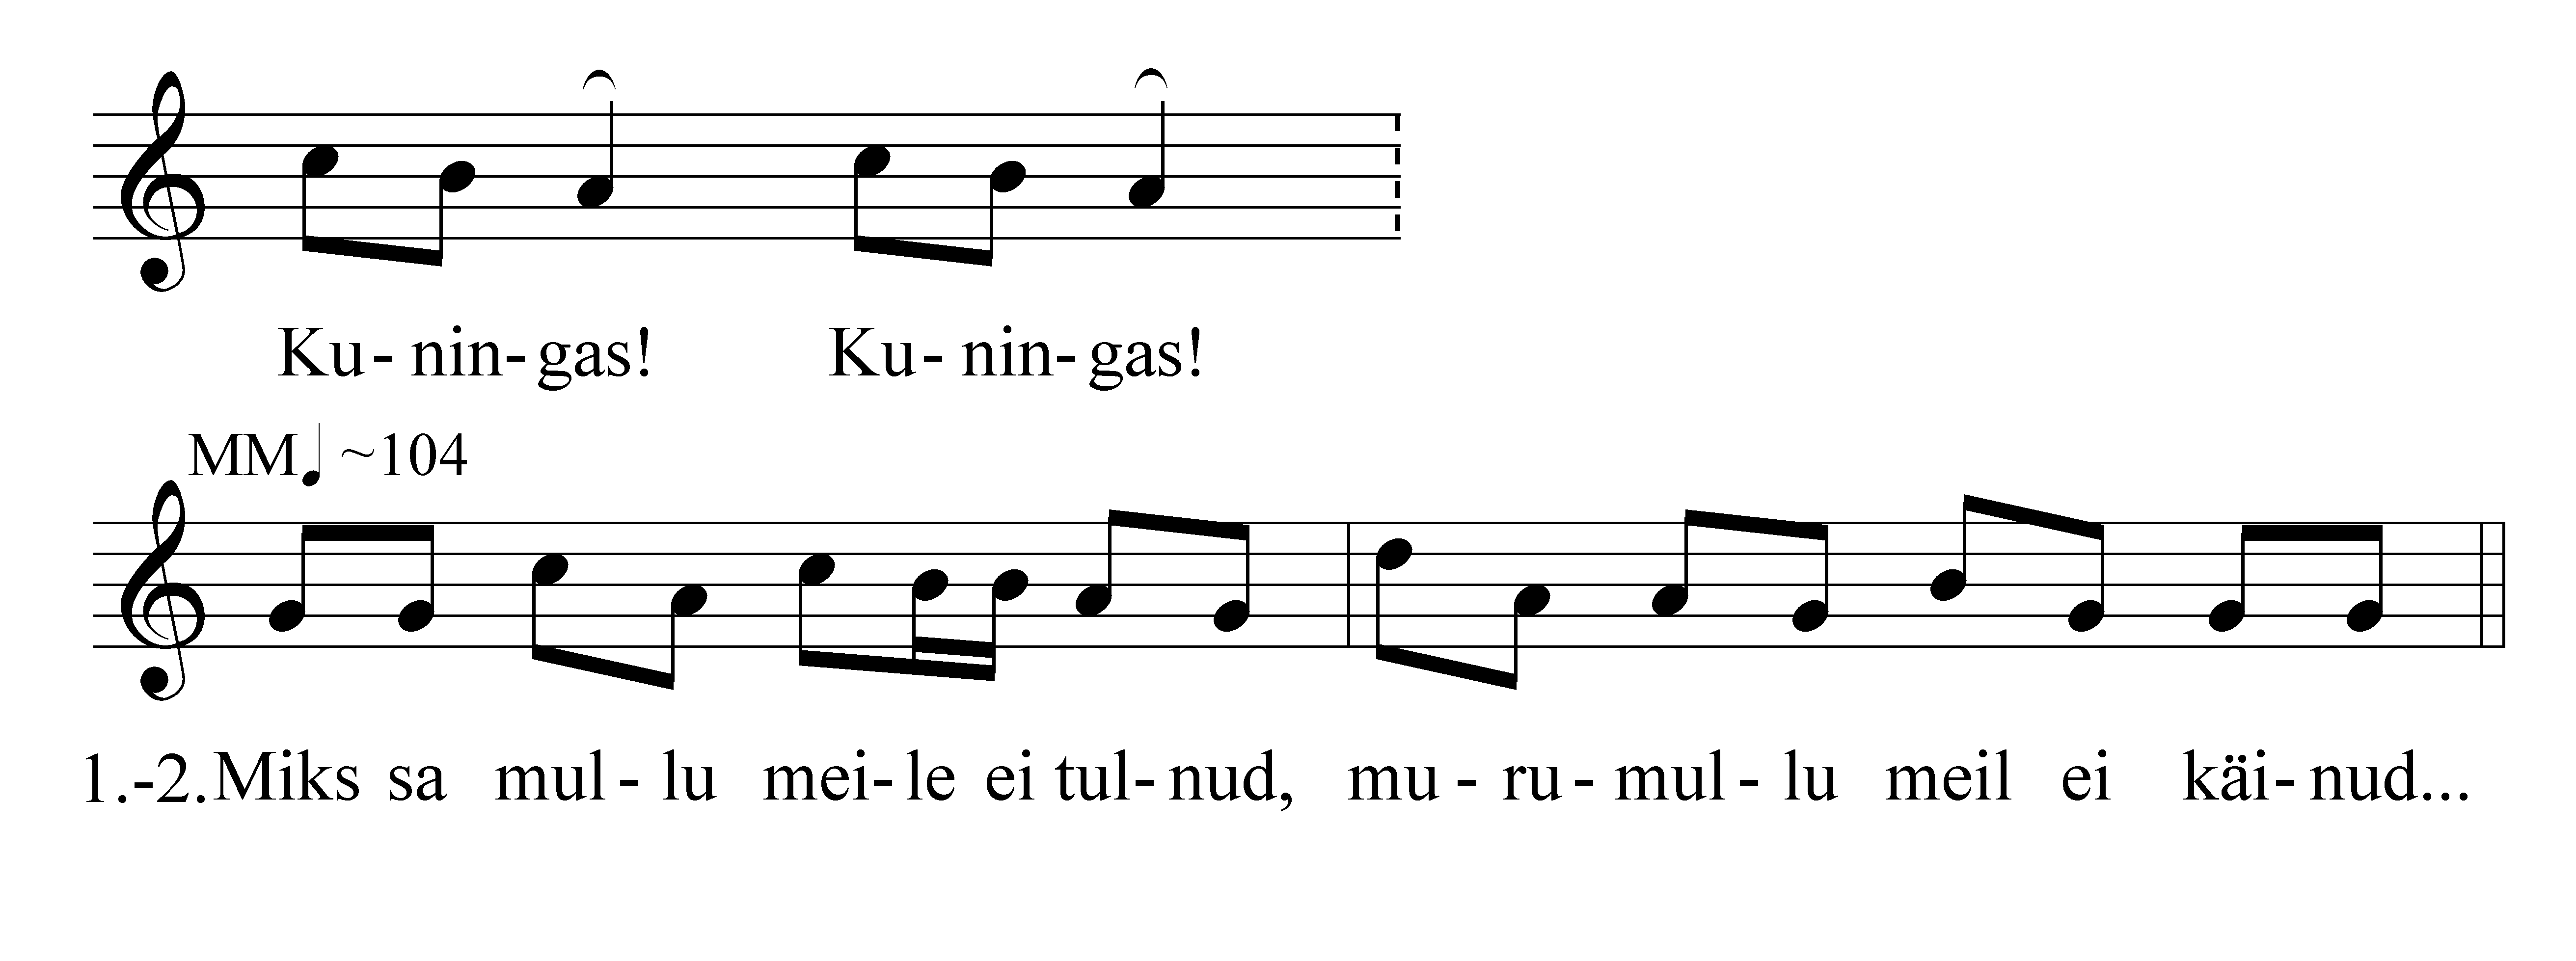
\includegraphics[width=300pt]{figures/094.png}
\caption{Kuningamäng ``The King Game" performed by Liisa Kümmel}
\label{song 94}
\end{center}
\end{figure}


\begin{figure}[htbp]
\begin{center}
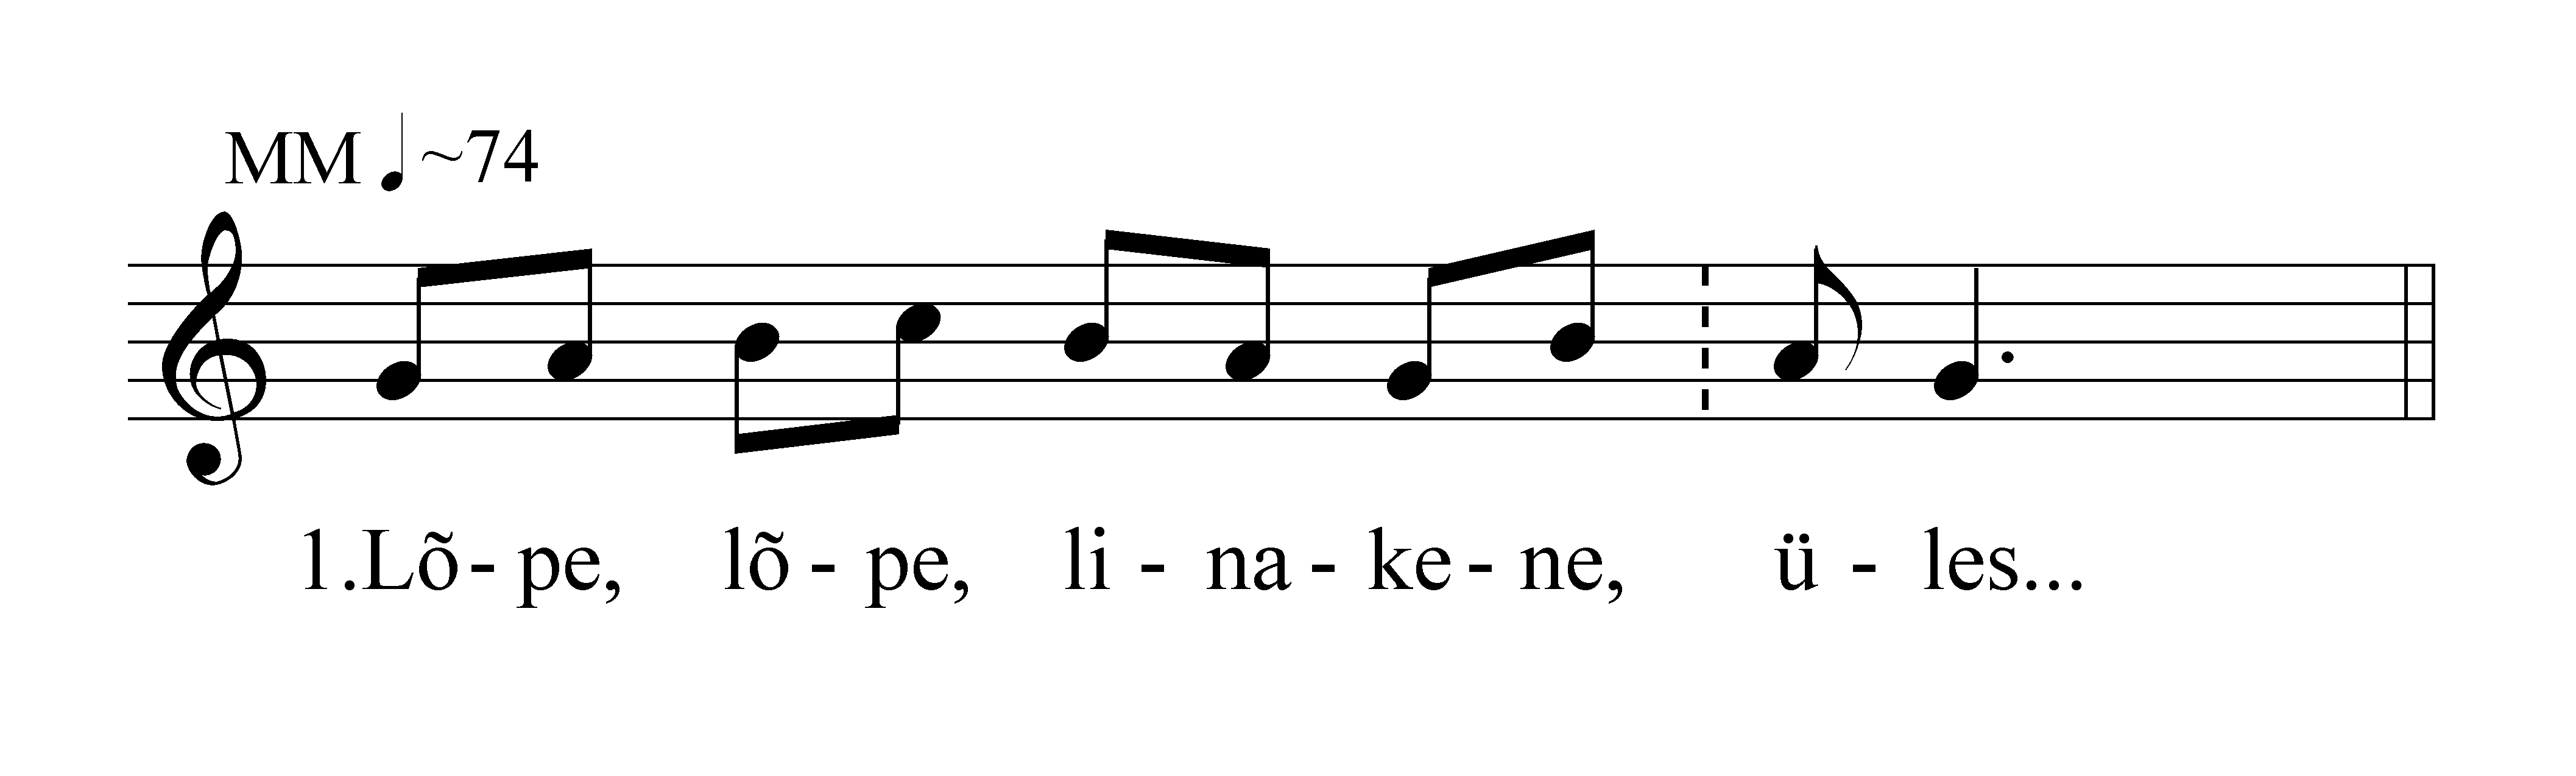
\includegraphics[width=300pt]{figures/009.png}
\caption{Põld lindudele performed by Marie Helimets}
\label{song 9 }
\end{center}
\end{figure}


\begin{figure}[htbp]
\begin{center}
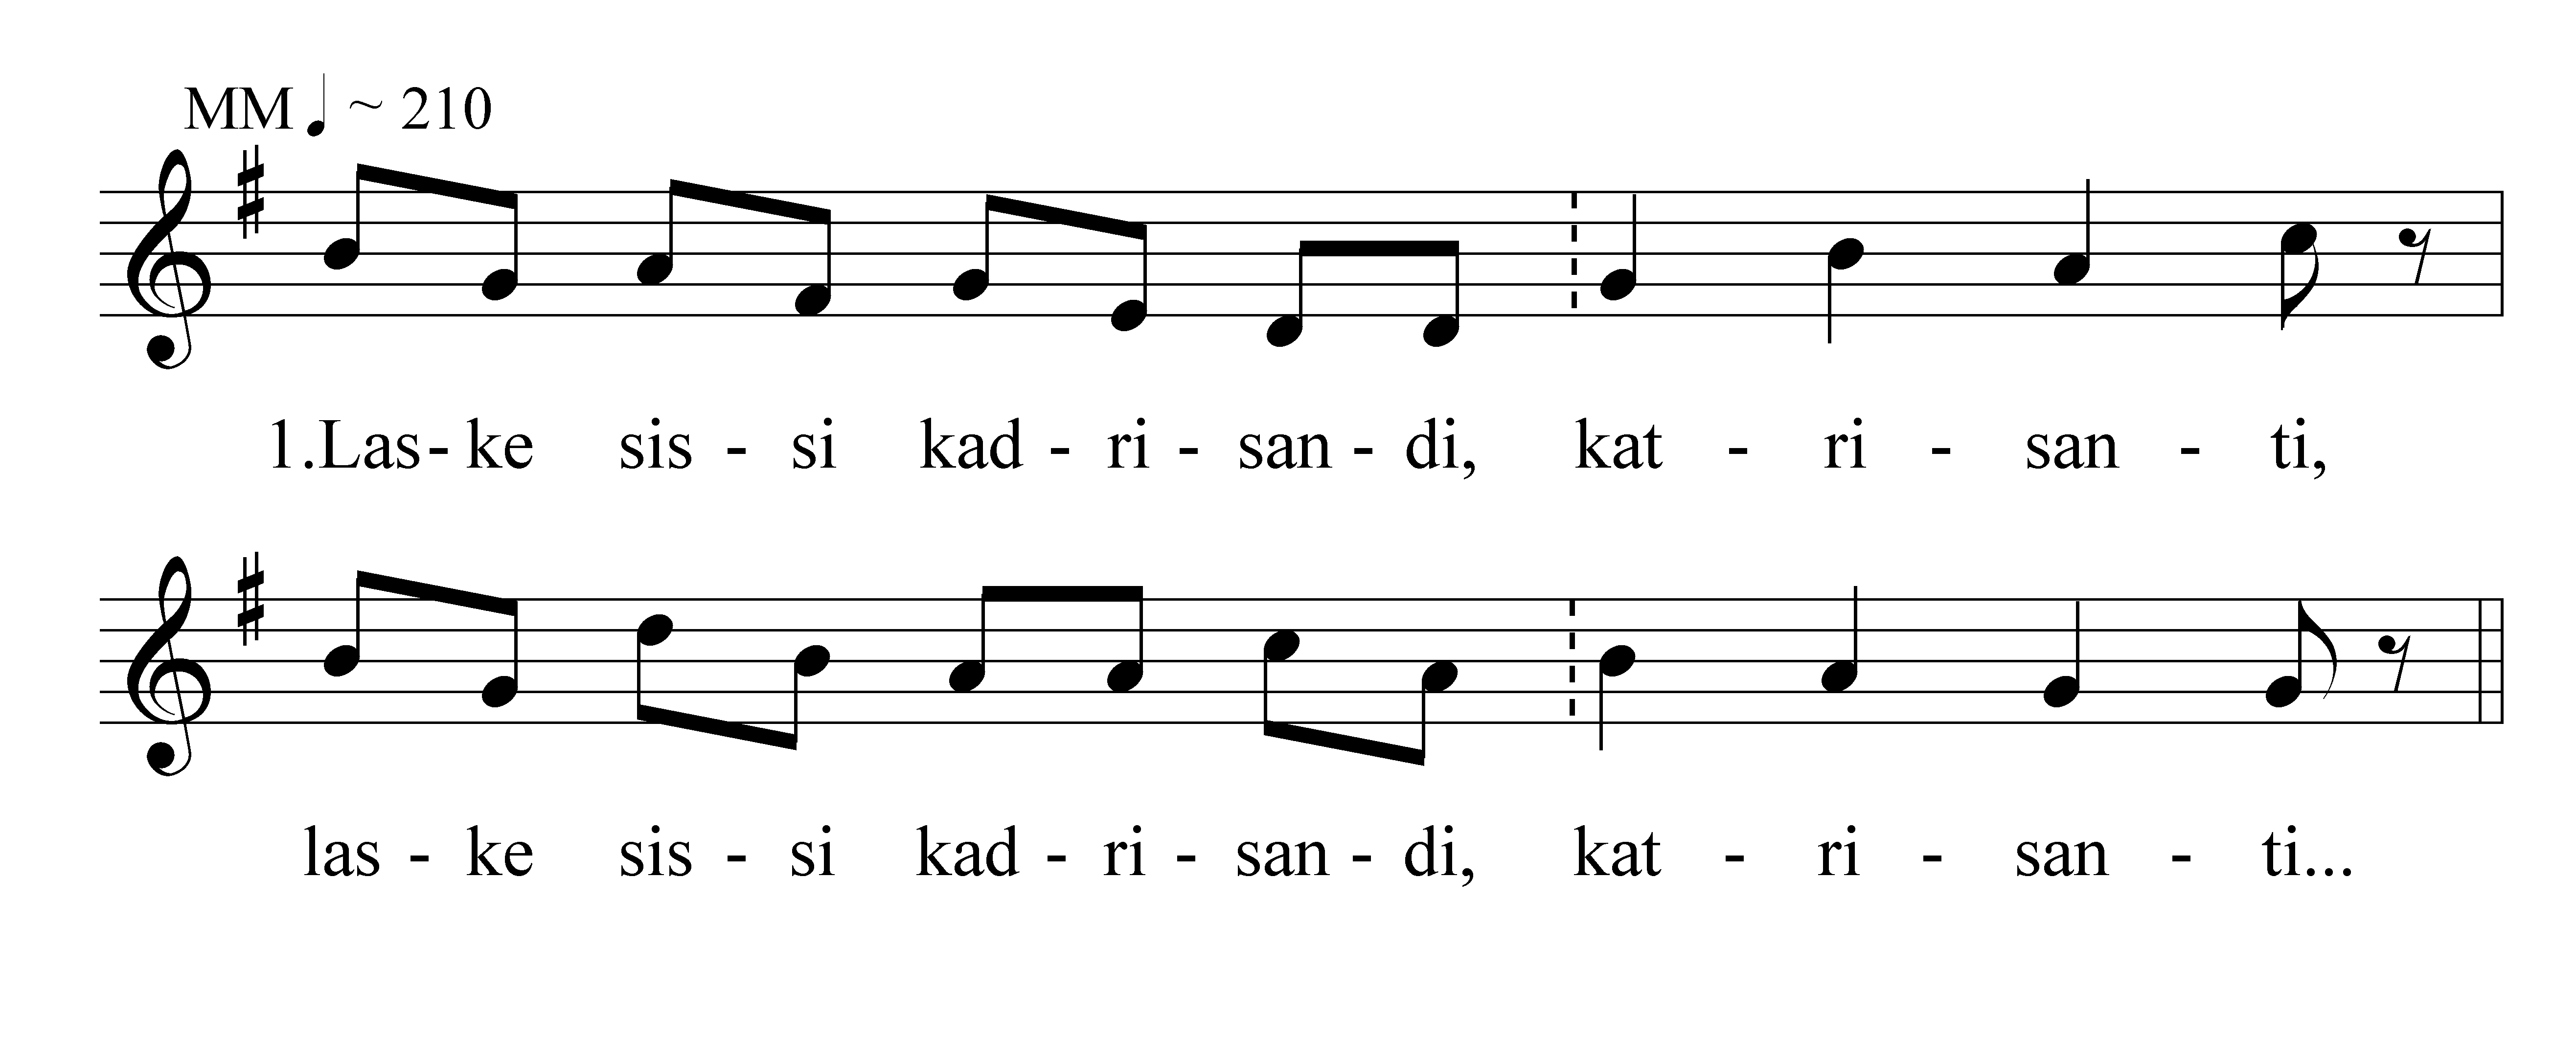
\includegraphics[width=300pt]{figures/018.png}
\caption{Kadrilaul performed by Marie Helimets}
\label{song 18}
\end{center}
\end{figure}


\begin{figure}[htbp]
\begin{center}
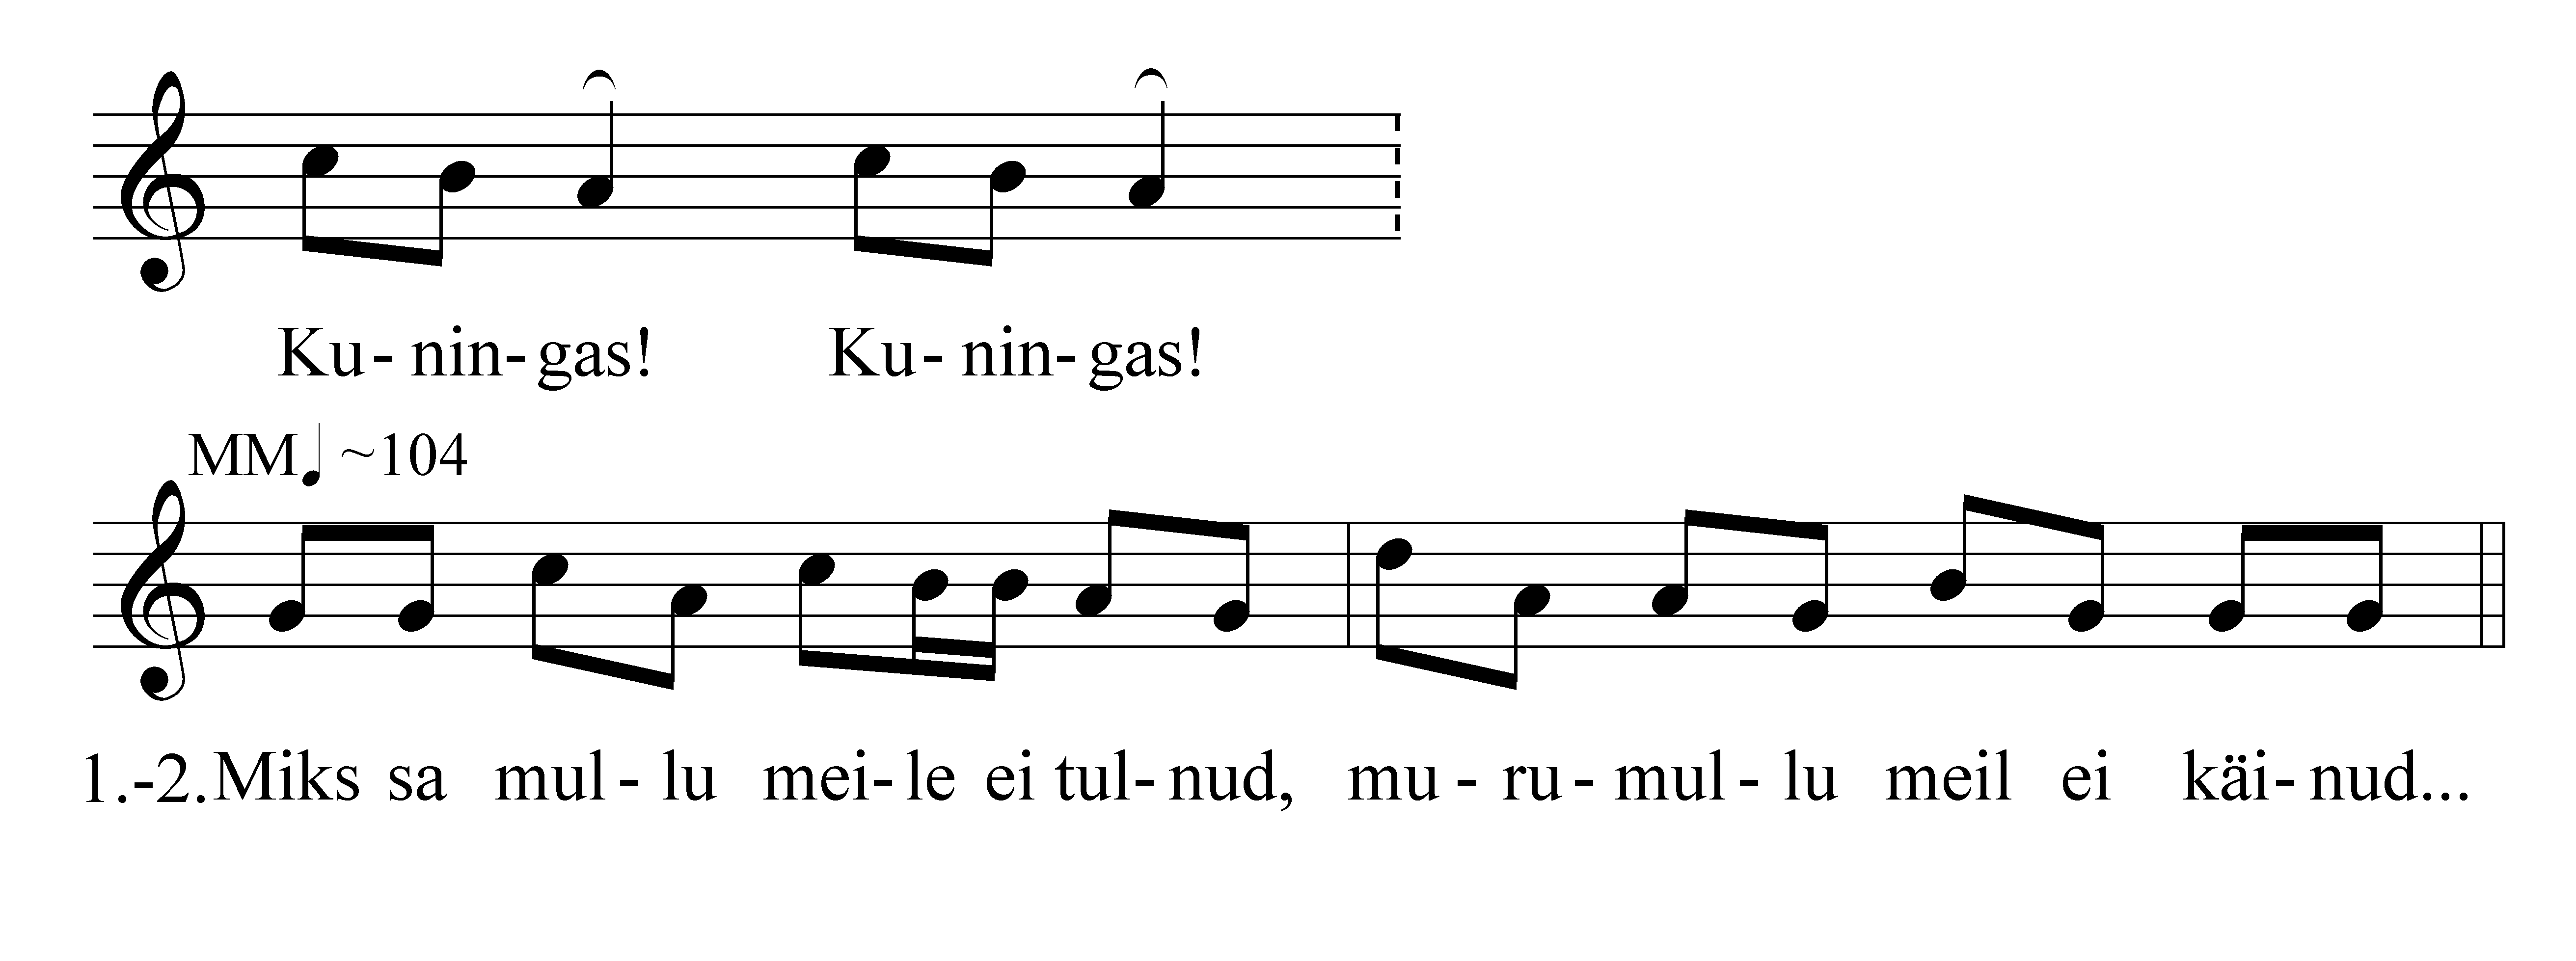
\includegraphics[width=300pt]{figures/094.png}
\caption{default}
\label{94}
\end{center}
\end{figure}


\begin{figure}[htbp]
\begin{center}
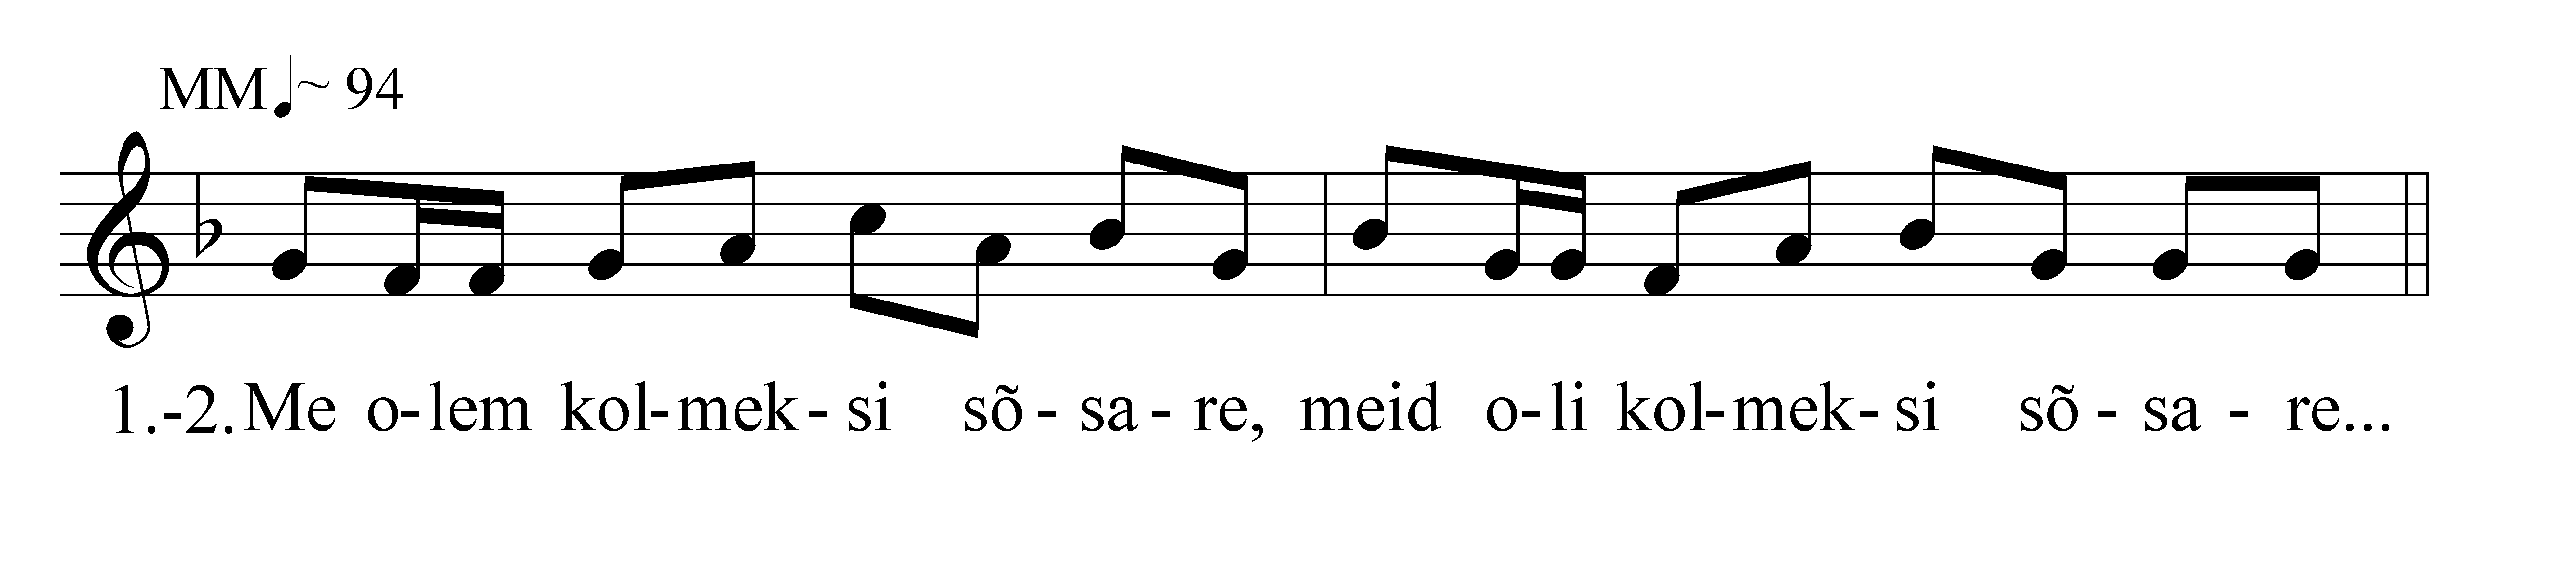
\includegraphics[width=300pt]{figures/081.png}
\caption{Mehetapja (Maielaul) Greete Jents}
\label{81}
\end{center}
\end{figure}


\begin{figure}[htbp]
\begin{center}
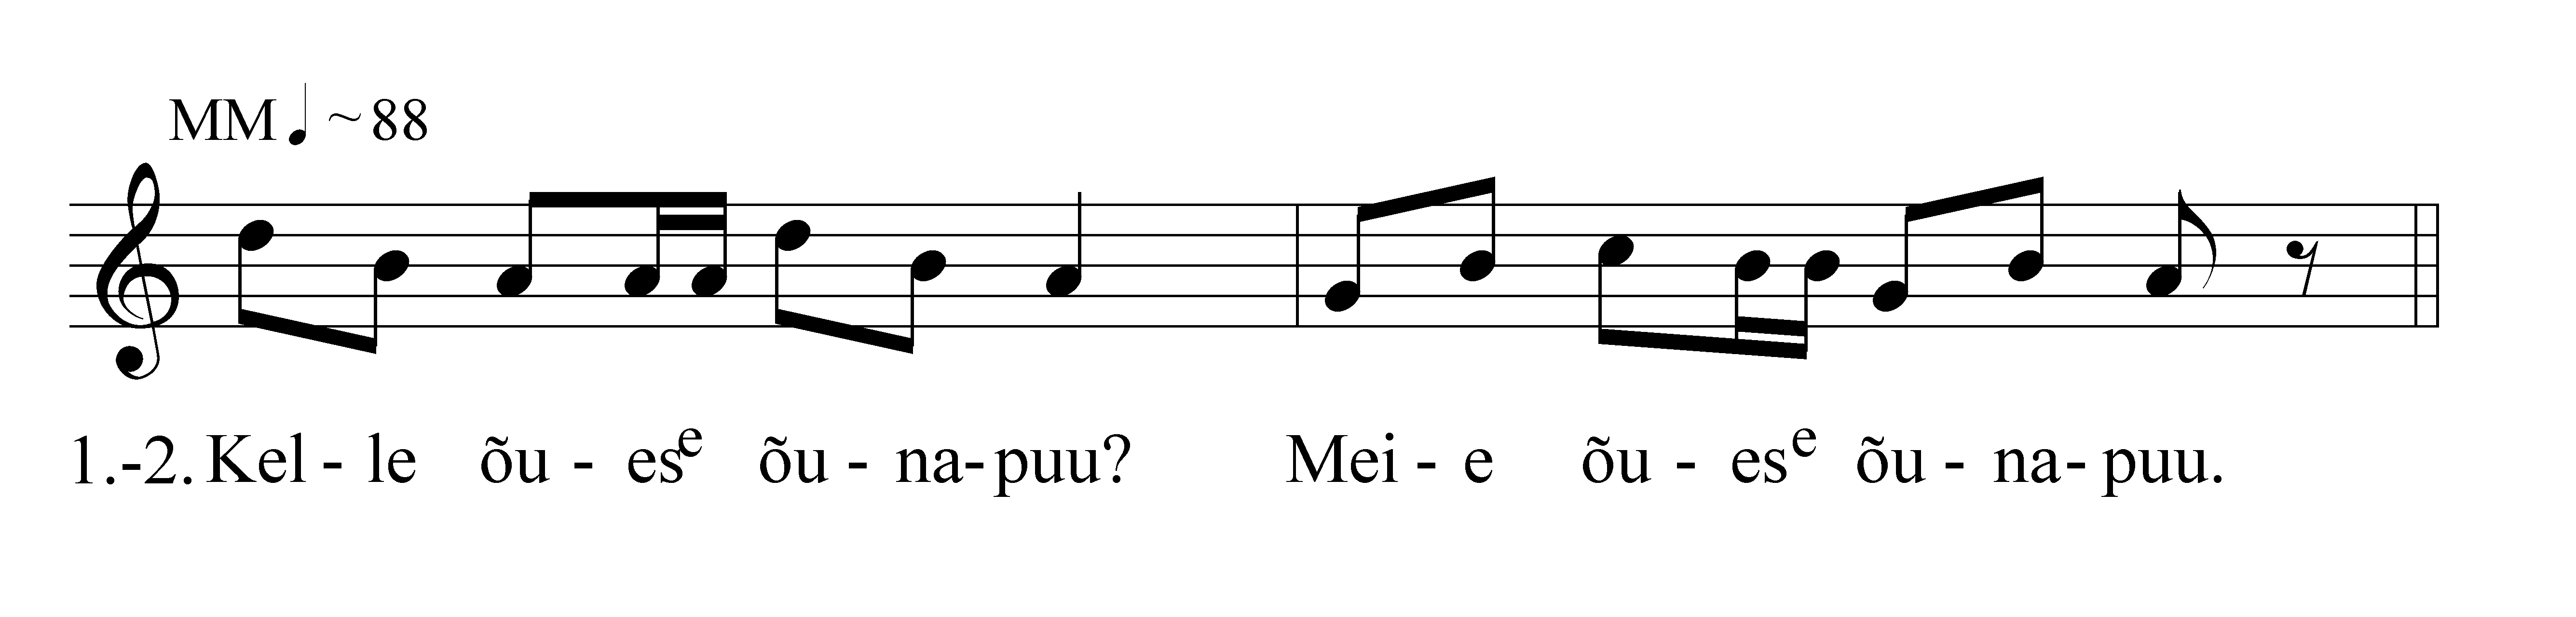
\includegraphics[width=300pt]{figures/077.png}
\caption{{\it Loomine} performed by Liisu Orik }
\label{77}
\end{center}
\end{figure}

\begin{figure}[htbp]
\begin{center}
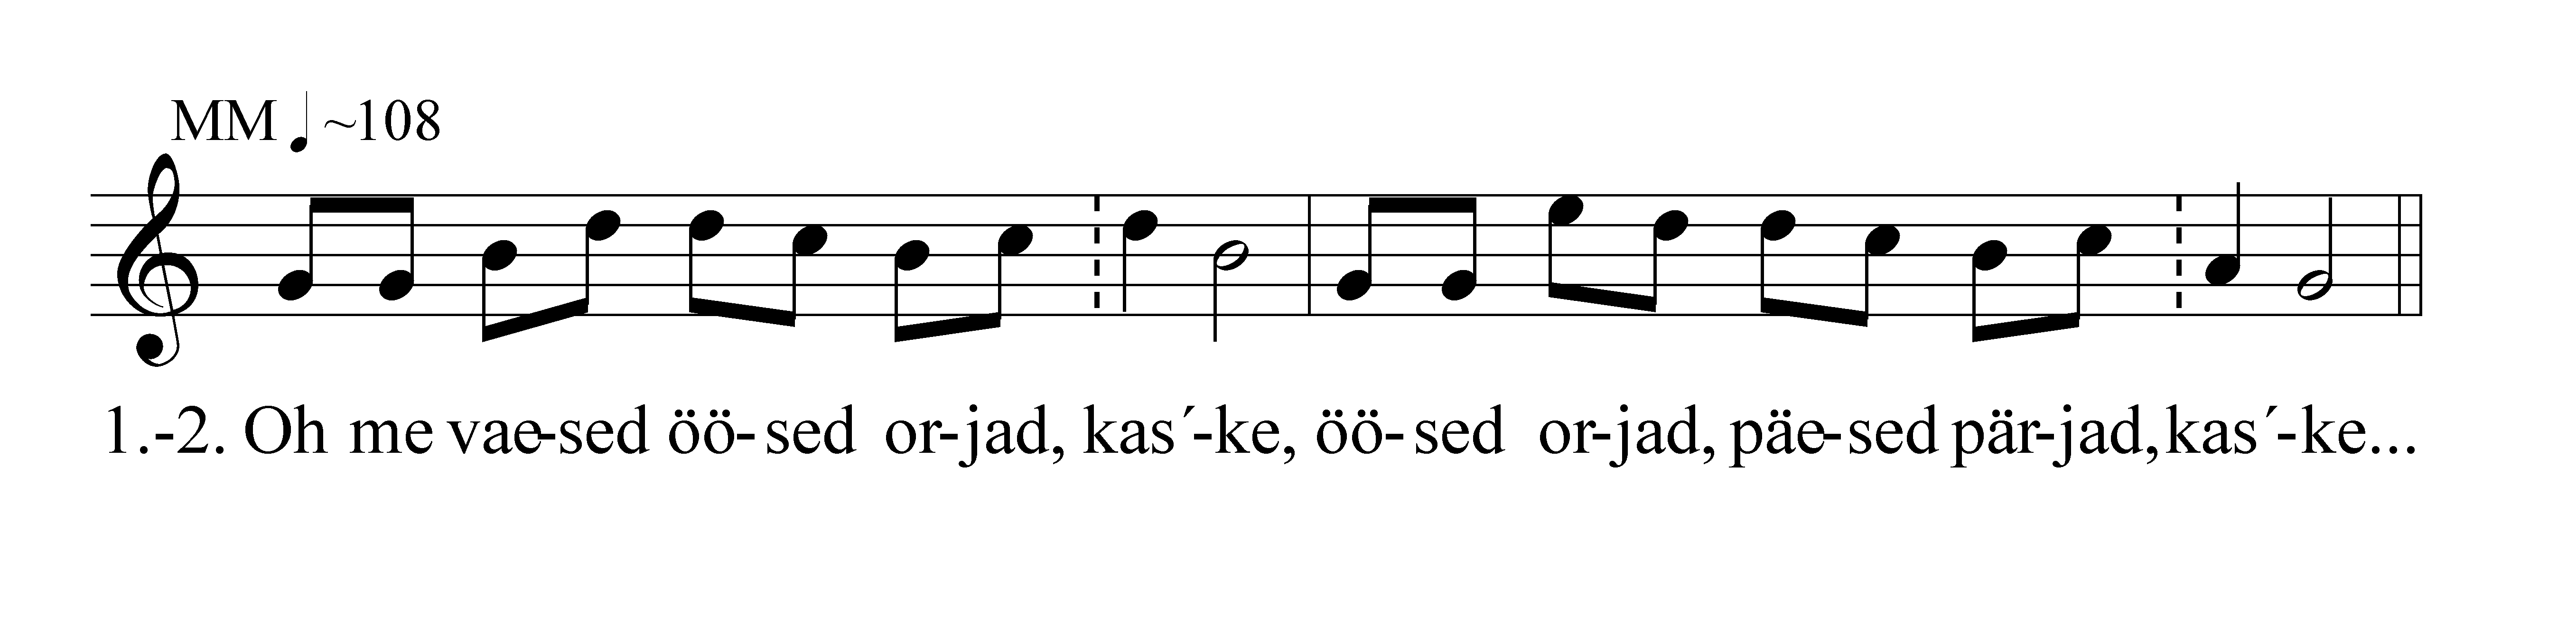
\includegraphics[width=300pt]{figures/069.png}
\caption{default}
\label{default}
\end{center}
\end{figure}

\begin{figure}[htbp]
\begin{center}
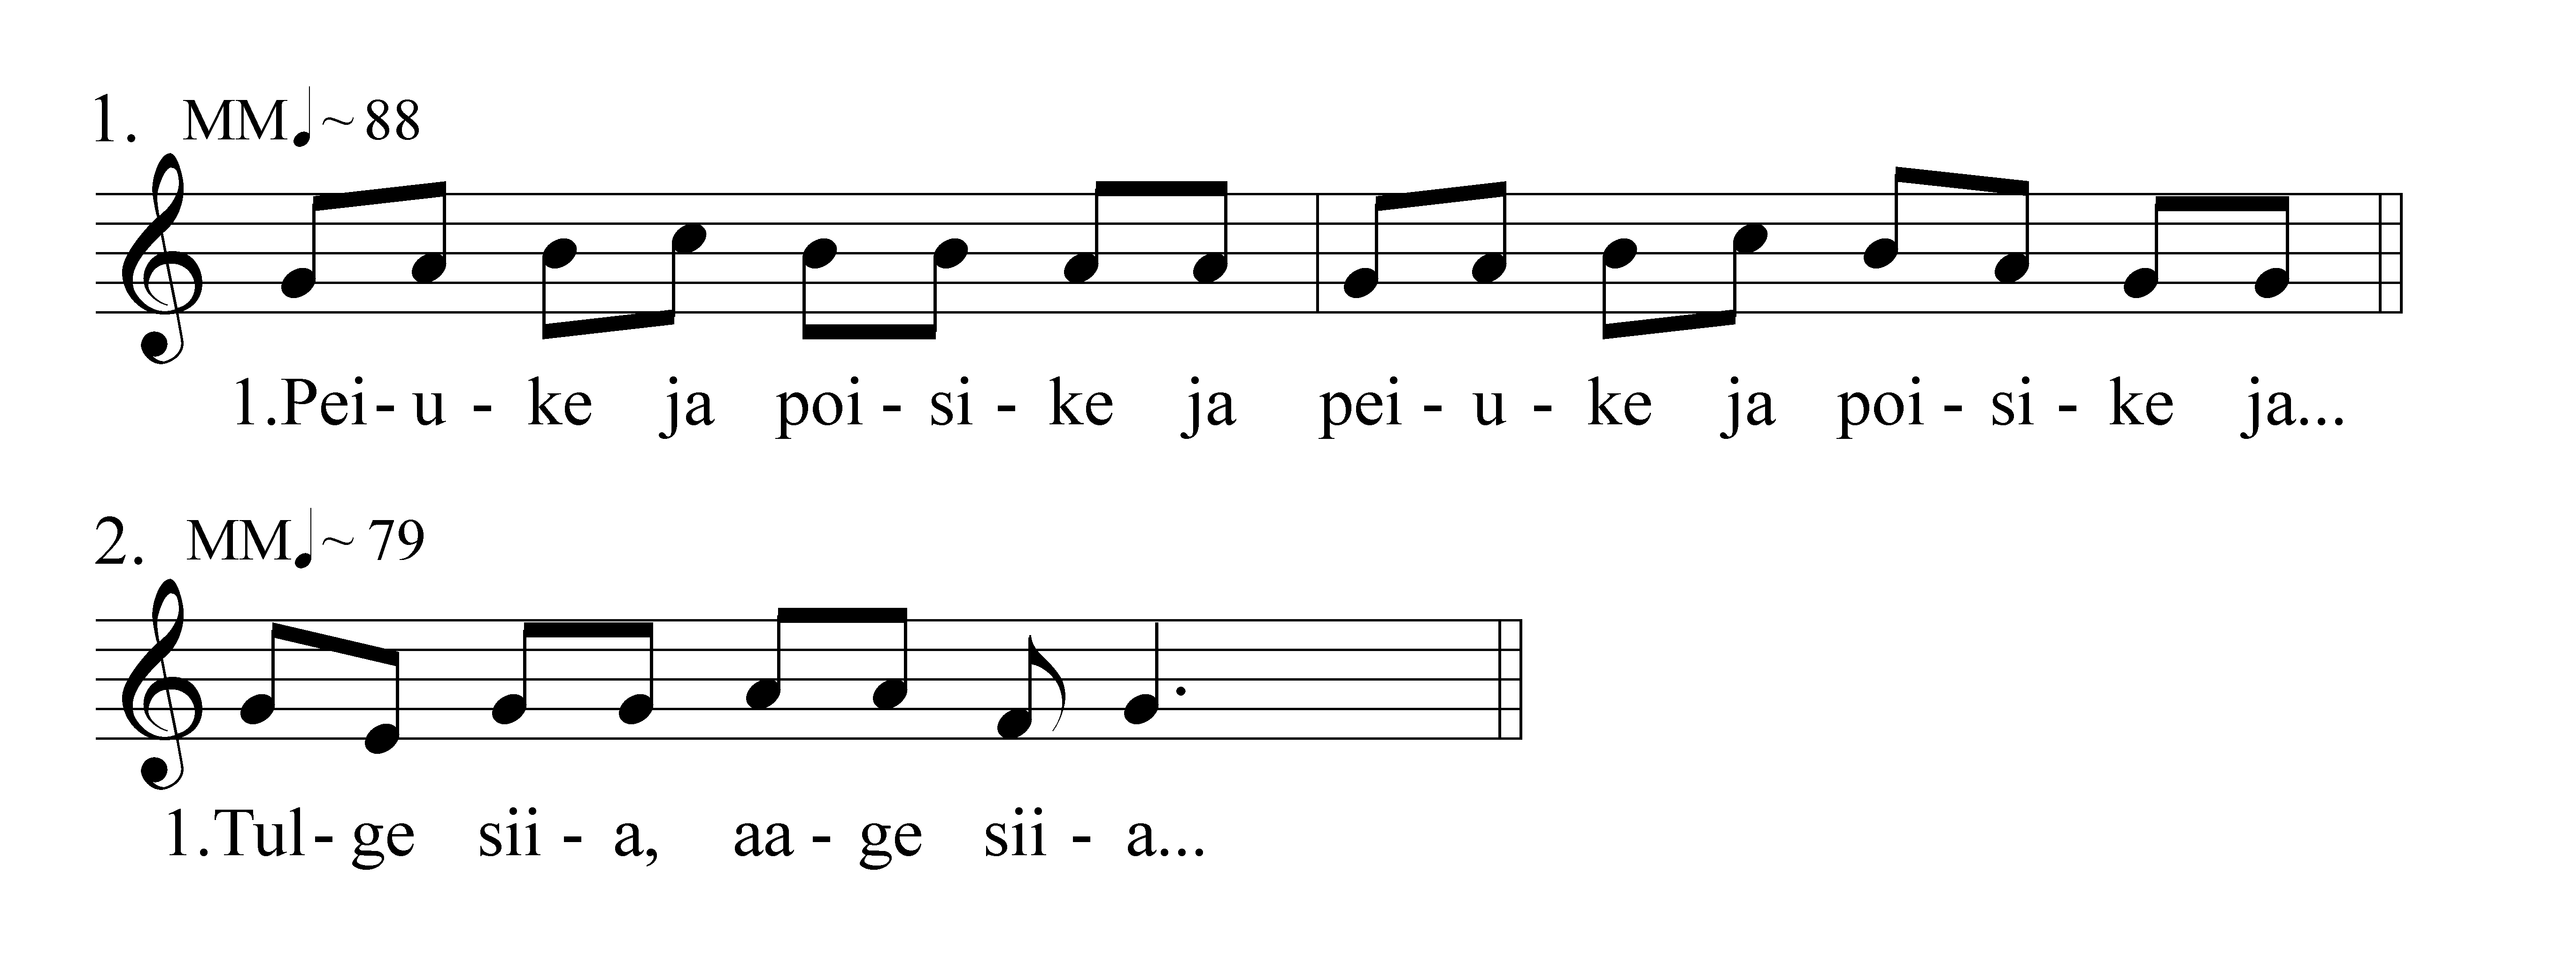
\includegraphics[width=300pt]{figures/045.png}
\caption{default}
\label{default}
\end{center}
\end{figure}






\begin{figure}[htbp]
\begin{center}
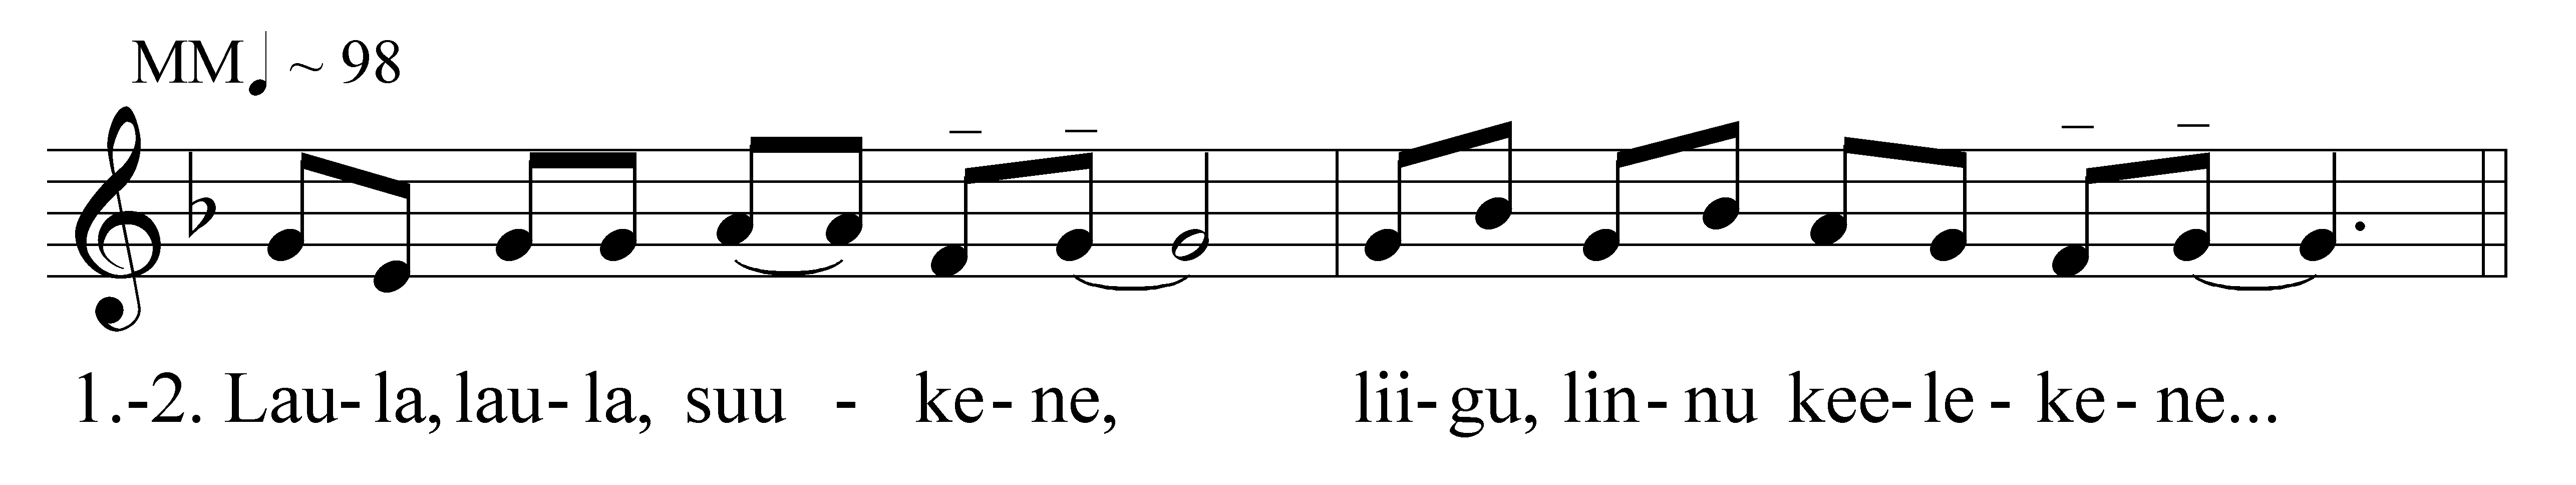
\includegraphics[width=300pt]{figures/055.png}
\caption{default}
\label{default}
\end{center}
\end{figure}



\begin{figure}[htbp]
\begin{center}
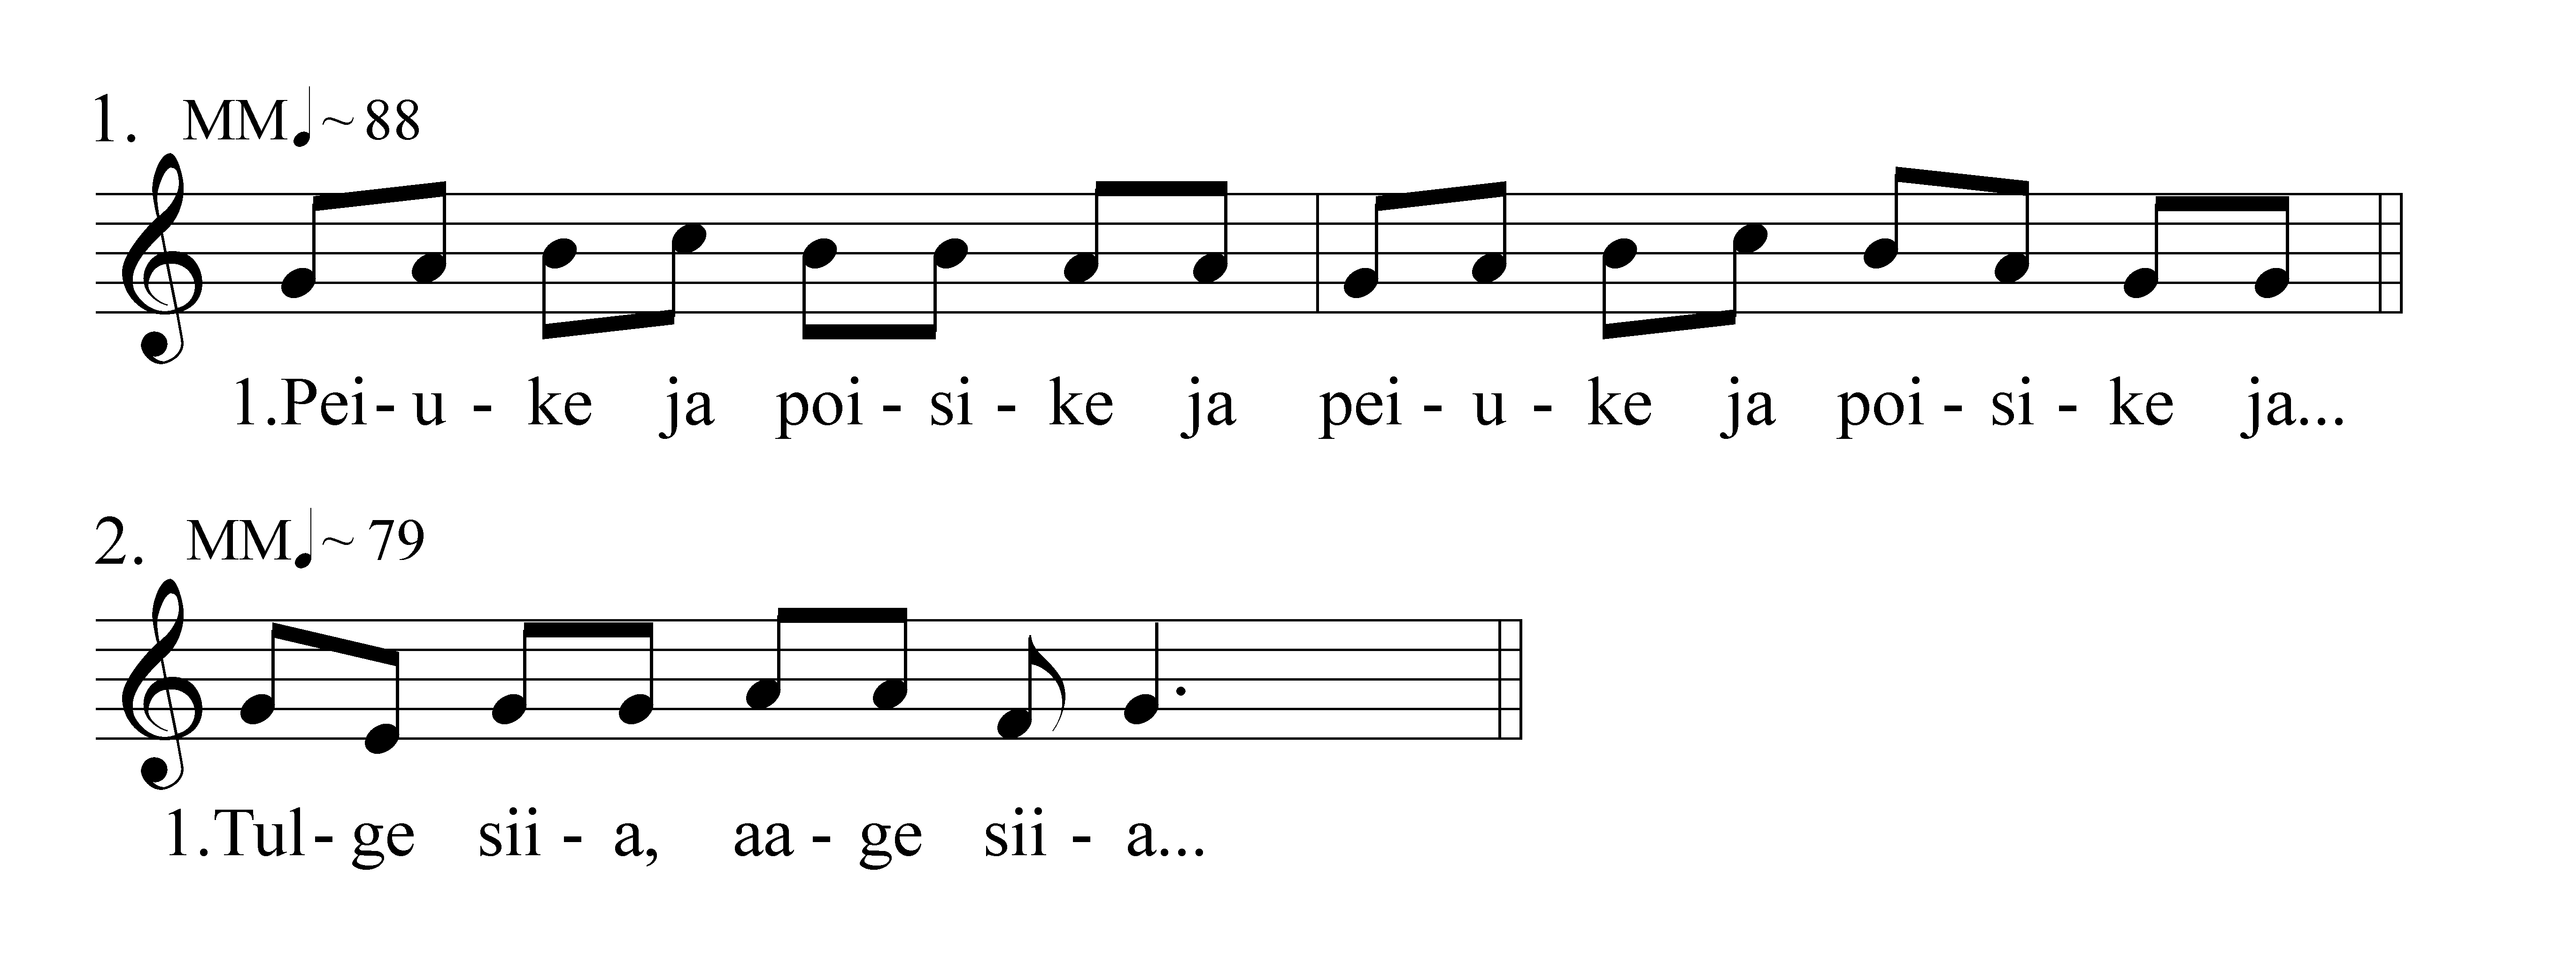
\includegraphics[width=300pt]{figures/045.png}
\caption{default}
\label{default}
\end{center}
\end{figure}
%\chapter{Estonian Folklore Archives}
\begin{figure}[htb]
\begin{center}
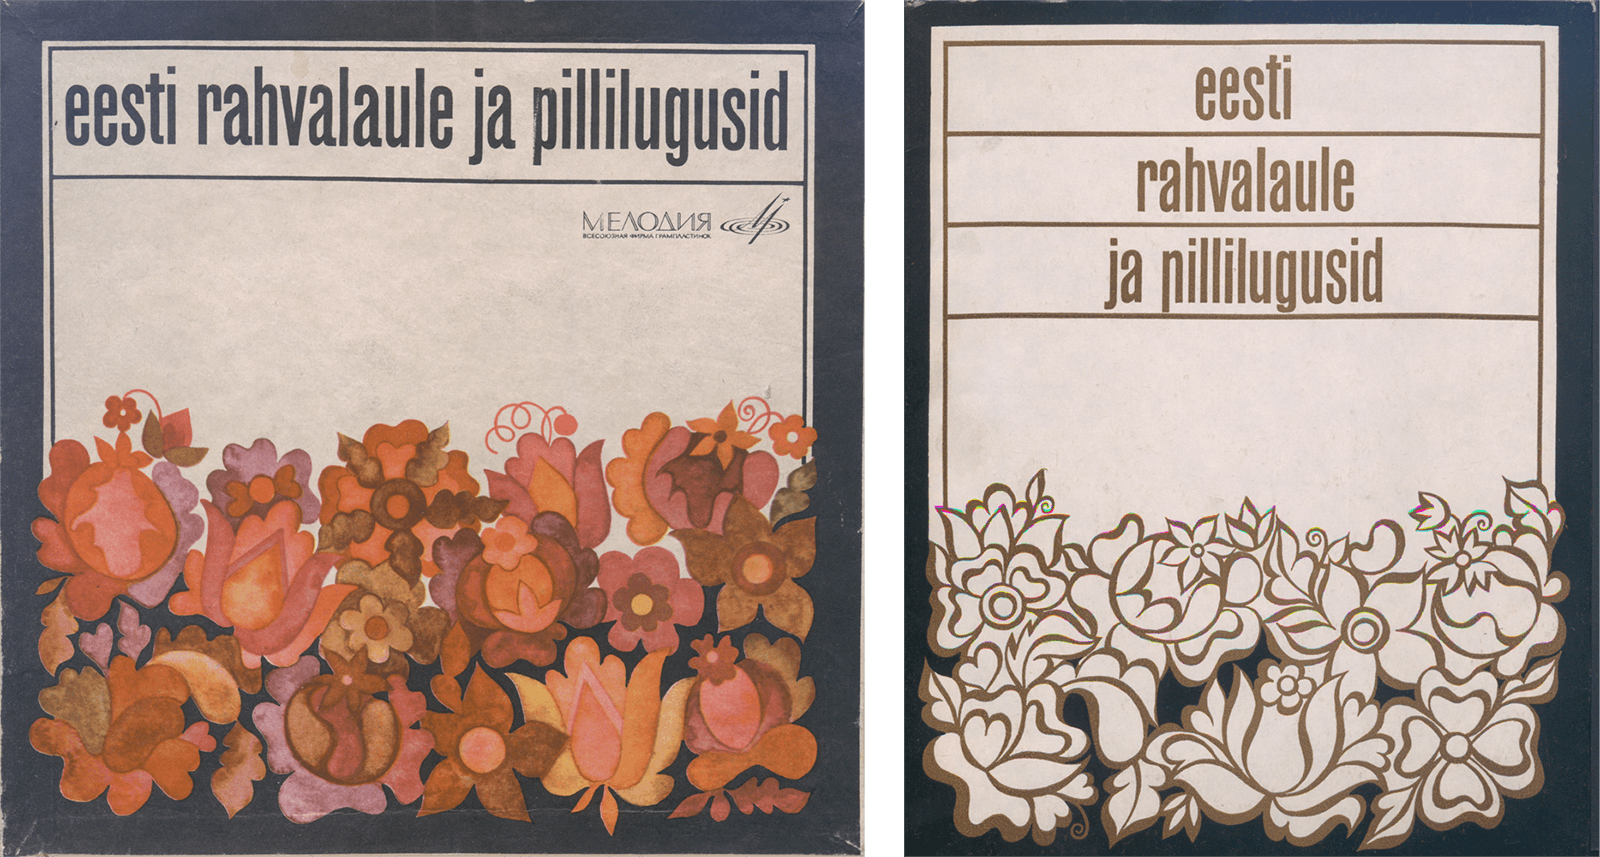
\includegraphics[width=300pt]{figures/vinyyl.png}
\caption{1970 cover art of vinyl anthology}
\label{vinyl1970}
\end{center}
\end{figure}

\begin{figure}[htp]
\centering
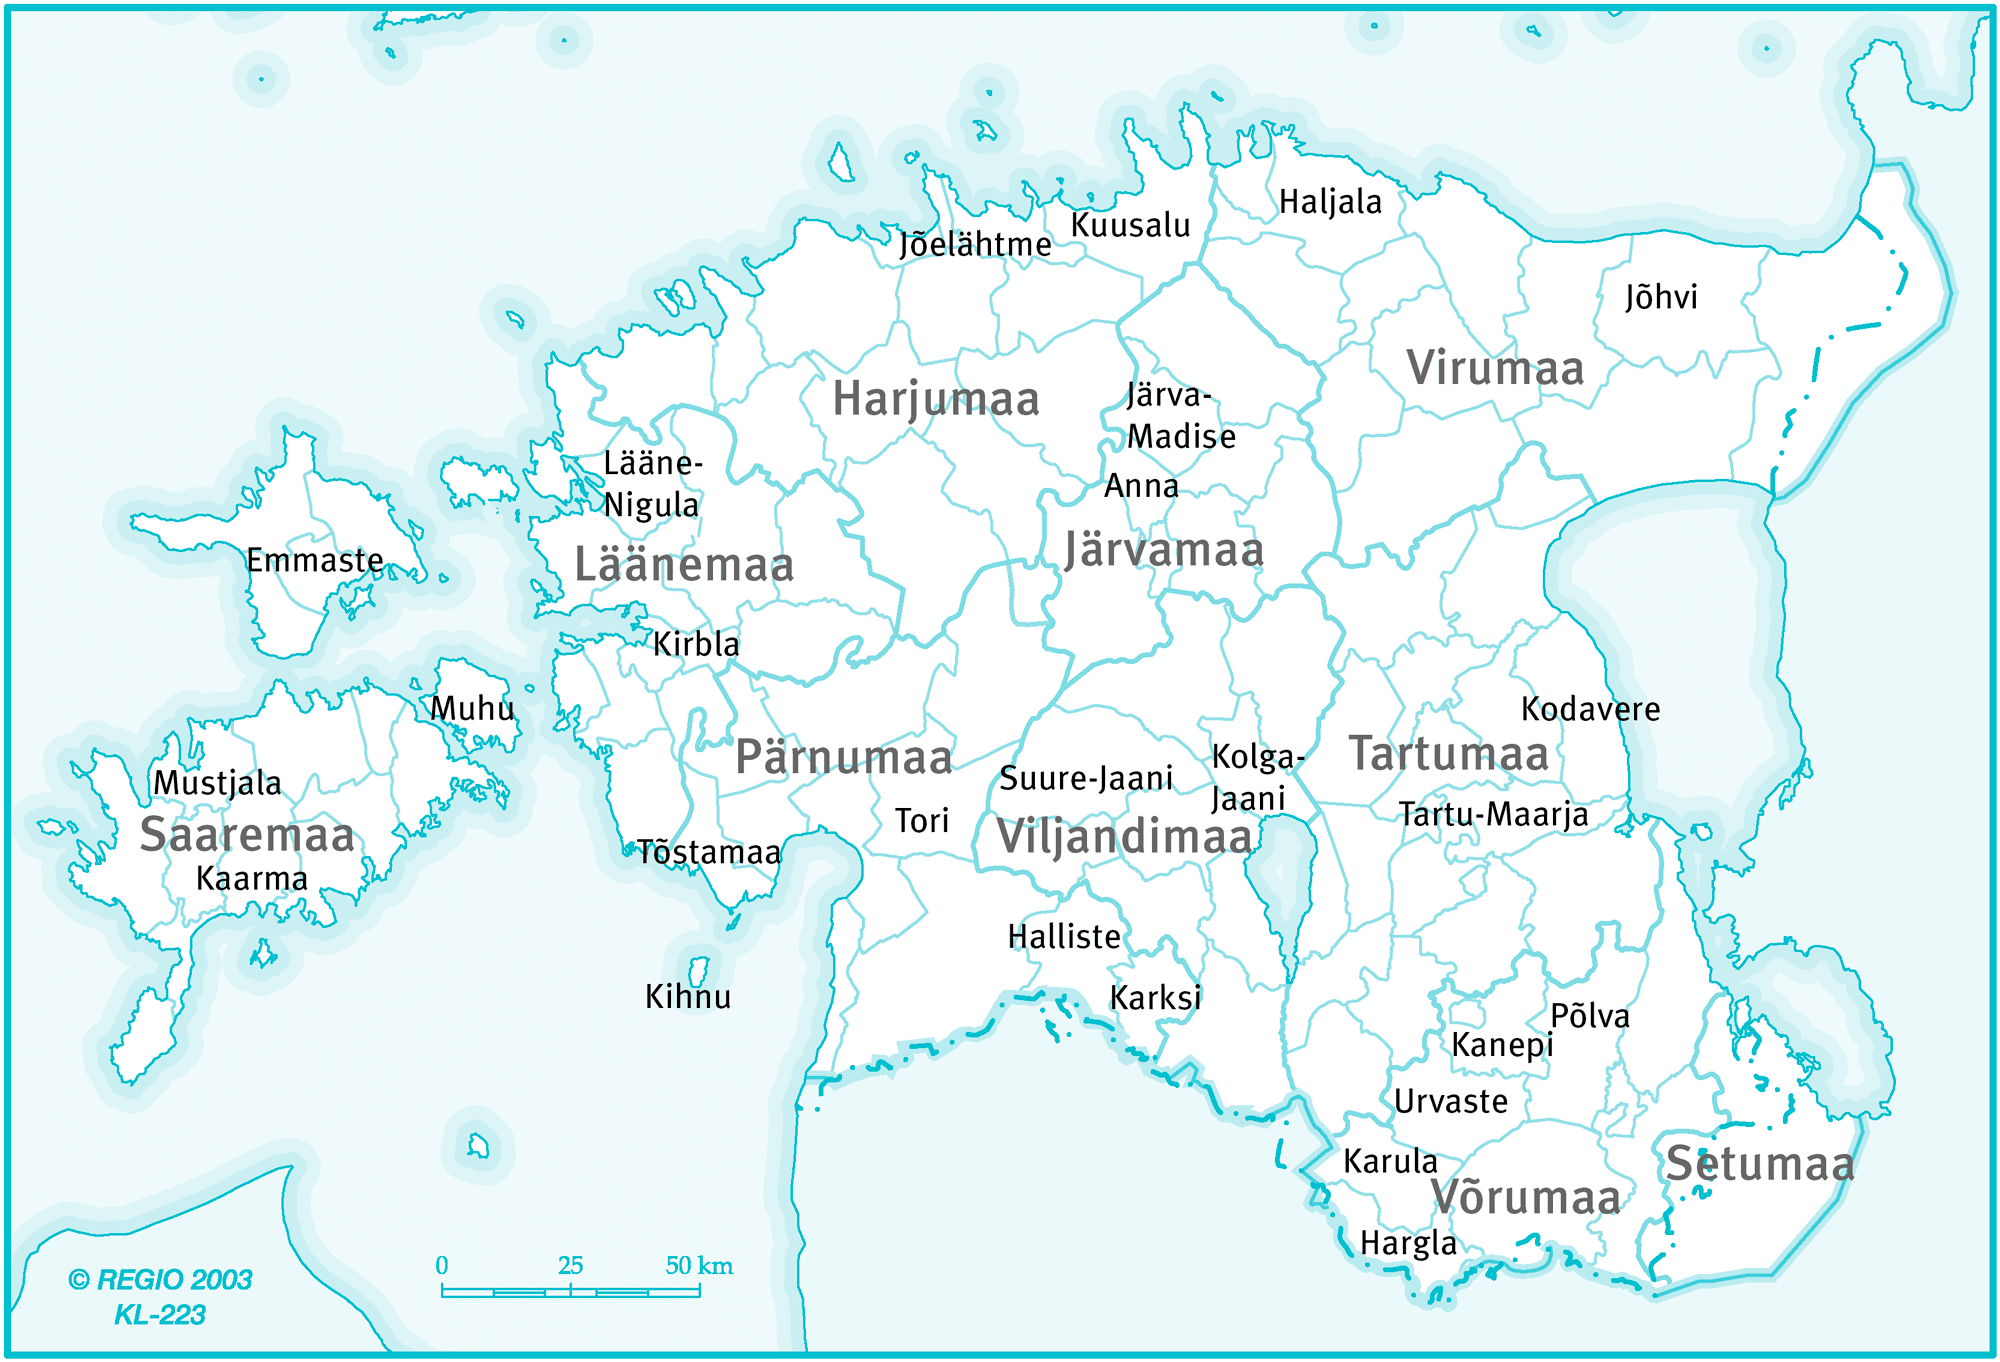
\includegraphics[width=0.9\linewidth]{figures/kihelkonnad}
\end{figure} 

%%song only
% latex table generated in R 4.1.2 by xtable 1.8-4 package
% Fri Aug 12 21:55:13 2022
\begin{longtable}{lrrrrrrrr}
  \toprule
Parameter & Rhat & n\_eff & mean & sd & se\_mean & 2.5\% & 50\% & 97.5\% \\ 
  \midrule
Intercept & 1.001 &  801 & 0.193 & 0.024 & 0.001 & 0.143 & 0.194 & 0.242 \\ 
  ictusoff & 1.000 & 4507 & -0.016 & 0.006 & 0.000 & -0.028 & -0.016 & -0.003 \\ 
  stressed1 & 1.001 & 4042 & 0.047 & 0.007 & 0.000 & 0.034 & 0.047 & 0.060 \\ 
  quantity2 & 1.002 & 3755 & -0.025 & 0.007 & 0.000 & -0.039 & -0.025 & -0.012 \\ 
  quantity3 & 1.002 & 3613 & -0.037 & 0.011 & 0.000 & -0.058 & -0.037 & -0.016 \\ 
  b[(Intercept) song:9] & 1.001 &  889 & 0.094 & 0.025 & 0.001 & 0.044 & 0.093 & 0.145 \\ 
  b[(Intercept) song:18] & 1.001 &  799 & -0.006 & 0.024 & 0.001 & -0.054 & -0.006 & 0.043 \\ 
  b[(Intercept) song:41] & 1.001 &  830 & 0.022 & 0.025 & 0.001 & -0.028 & 0.022 & 0.073 \\ 
  b[(Intercept) song:55] & 1.001 &  846 & -0.037 & 0.026 & 0.001 & -0.088 & -0.036 & 0.015 \\ 
  b[(Intercept) song:65] & 1.001 &  860 & 0.075 & 0.025 & 0.001 & 0.025 & 0.075 & 0.125 \\ 
  b[(Intercept) song:69] & 1.000 & 1211 & -0.042 & 0.031 & 0.001 & -0.105 & -0.042 & 0.016 \\ 
  b[(Intercept) song:77] & 1.001 &  993 & -0.105 & 0.027 & 0.001 & -0.159 & -0.105 & -0.051 \\ 
  b[(Intercept) song:92] & 1.001 &  989 & 0.033 & 0.027 & 0.001 & -0.020 & 0.034 & 0.087 \\ 
  b[(Intercept) song:94] & 1.002 &  878 & -0.039 & 0.025 & 0.001 & -0.089 & -0.039 & 0.011 \\ 
   \bottomrule
\caption{posterier parameters} 
\end{longtable}


%performer & word

% latex table generated in R 4.1.2 by xtable 1.8-4 package
% Fri Aug 12 19:59:47 2022
\begin{longtable}{lrrrrrrr}
  \toprule
Parameter & Rhat & n\_eff & mean & sd & 2.5\% & 50\% & 97.5\% \\ 
  \midrule
Intercept & 1.000 & 1871 & 0.197 & 0.036 & 0.122 & 0.197 & 0.270 \\ 
  ictusoff & 1.000 & 4383 & -0.022 & 0.007 & -0.035 & -0.022 & -0.008 \\ 
  stressed1 & 0.999 & 5726 & 0.050 & 0.006 & 0.038 & 0.050 & 0.062 \\ 
  quantity2 & 0.999 & 4036 & -0.029 & 0.007 & -0.043 & -0.029 & -0.015 \\ 
  quantity3 & 0.999 & 3106 & -0.036 & 0.013 & -0.062 & -0.036 & -0.010 \\ 
  b[(Intercept) word:ää] & 1.000 & 3916 & 0.143 & 0.043 & 0.058 & 0.142 & 0.228 \\ 
  b[(Intercept) word:aga] & 1.000 & 6184 & -0.065 & 0.034 & -0.133 & -0.065 & 0.001 \\ 
  b[(Intercept) word:ahju] & 1.000 & 8703 & -0.020 & 0.034 & -0.088 & -0.021 & 0.047 \\ 
  b[(Intercept) word:aia] & 1.000 & 7218 & 0.034 & 0.040 & -0.043 & 0.034 & 0.112 \\ 
  b[(Intercept) word:ajal,] & 1.000 & 7275 & 0.009 & 0.034 & -0.058 & 0.008 & 0.078 \\ 
  b[(Intercept) word:akkas] & 0.999 & 6375 & -0.032 & 0.034 & -0.101 & -0.032 & 0.035 \\ 
  b[(Intercept) word:allitagu,] & 0.999 & 7450 & 0.000 & 0.034 & -0.065 & 0.001 & 0.065 \\ 
  b[(Intercept) word:anisida,] & 1.000 & 7942 & 0.043 & 0.035 & -0.023 & 0.043 & 0.111 \\ 
  b[(Intercept) word:anna] & 0.999 & 7653 & 0.010 & 0.034 & -0.055 & 0.010 & 0.078 \\ 
  b[(Intercept) word:Anna,] & 1.000 & 7784 & -0.008 & 0.033 & -0.071 & -0.009 & 0.055 \\ 
  b[(Intercept) word:ärmätus] & 1.000 & 8103 & -0.021 & 0.034 & -0.086 & -0.020 & 0.043 \\ 
  b[(Intercept) word:Ega] & 1.000 & 6486 & -0.054 & 0.034 & -0.123 & -0.054 & 0.013 \\ 
  b[(Intercept) word:ei] & 1.000 & 6144 & -0.082 & 0.036 & -0.151 & -0.081 & -0.012 \\ 
  b[(Intercept) word:Ei] & 1.000 & 4695 & 0.120 & 0.043 & 0.037 & 0.120 & 0.203 \\ 
  b[(Intercept) word:esta!] & 0.999 & 7306 & -0.002 & 0.035 & -0.071 & -0.002 & 0.066 \\ 
  b[(Intercept) word:hääre] & 1.000 & 8670 & 0.017 & 0.034 & -0.051 & 0.018 & 0.084 \\ 
  b[(Intercept) word:halgu] & 1.000 & 8538 & -0.020 & 0.040 & -0.100 & -0.019 & 0.057 \\ 
  b[(Intercept) word:ilma,] & 0.999 & 8640 & 0.026 & 0.040 & -0.050 & 0.026 & 0.105 \\ 
  b[(Intercept) word:ilutse,] & 0.999 & 7301 & 0.021 & 0.034 & -0.047 & 0.021 & 0.088 \\ 
  b[(Intercept) word:ja] & 0.999 & 5985 & -0.067 & 0.031 & -0.129 & -0.066 & -0.008 \\ 
  b[(Intercept) word:jäi] & 0.999 & 7571 & -0.035 & 0.041 & -0.119 & -0.036 & 0.045 \\ 
  b[(Intercept) word:jalas] & 1.000 & 7026 & 0.029 & 0.034 & -0.036 & 0.029 & 0.095 \\ 
  b[(Intercept) word:jätan] & 1.000 & 7693 & 0.006 & 0.034 & -0.060 & 0.005 & 0.072 \\ 
  b[(Intercept) word:jätän] & 0.999 & 8537 & -0.005 & 0.035 & -0.074 & -0.005 & 0.063 \\ 
  b[(Intercept) word:Jätän] & 1.000 & 6625 & -0.011 & 0.034 & -0.078 & -0.011 & 0.058 \\ 
  b[(Intercept) word:jätan,] & 0.999 & 7348 & 0.050 & 0.034 & -0.015 & 0.051 & 0.116 \\ 
  b[(Intercept) word:juhate:] & 1.000 & 8309 & -0.022 & 0.034 & -0.086 & -0.022 & 0.043 \\ 
  b[(Intercept) word:juksimaie,] & 1.000 & 7291 & 0.023 & 0.033 & -0.041 & 0.023 & 0.088 \\ 
  b[(Intercept) word:julgust] & 1.000 & 6704 & -0.006 & 0.039 & -0.084 & -0.006 & 0.070 \\ 
  b[(Intercept) word:juure] & 0.999 & 6174 & 0.069 & 0.035 & -0.001 & 0.069 & 0.137 \\ 
  b[(Intercept) word:juuri] & 1.000 & 7542 & 0.031 & 0.032 & -0.032 & 0.031 & 0.094 \\ 
  b[(Intercept) word:Kadri] & 1.000 & 6946 & -0.070 & 0.035 & -0.138 & -0.070 & -0.001 \\ 
  b[(Intercept) word:kadril] & 1.000 & 7841 & 0.010 & 0.033 & -0.055 & 0.009 & 0.075 \\ 
  b[(Intercept) word:kadrisandi,] & 0.999 & 8674 & 0.004 & 0.027 & -0.049 & 0.004 & 0.058 \\ 
  b[(Intercept) word:kaelakardasida,] & 1.000 & 7210 & 0.003 & 0.033 & -0.064 & 0.003 & 0.068 \\ 
  b[(Intercept) word:käinud,] & 1.001 & 7140 & -0.042 & 0.034 & -0.108 & -0.042 & 0.025 \\ 
  b[(Intercept) word:käisid] & 0.999 & 7889 & -0.044 & 0.034 & -0.112 & -0.044 & 0.024 \\ 
  b[(Intercept) word:kakud] & 1.000 & 7280 & -0.058 & 0.034 & -0.124 & -0.057 & 0.008 \\ 
  b[(Intercept) word:kambren] & 1.000 & 7709 & -0.028 & 0.034 & -0.095 & -0.029 & 0.041 \\ 
  b[(Intercept) word:kana] & 1.000 & 8581 & 0.003 & 0.034 & -0.063 & 0.003 & 0.070 \\ 
  b[(Intercept) word:kanaliha\_–] & 1.000 & 7102 & 0.010 & 0.034 & -0.055 & 0.010 & 0.075 \\ 
  b[(Intercept) word:kandijaksa,] & 1.000 & 7895 & 0.004 & 0.034 & -0.063 & 0.003 & 0.071 \\ 
  b[(Intercept) word:kannustenu.] & 0.999 & 7820 & -0.021 & 0.034 & -0.087 & -0.021 & 0.045 \\ 
  b[(Intercept) word:kapi] & 1.000 & 7349 & -0.004 & 0.034 & -0.072 & -0.003 & 0.062 \\ 
  b[(Intercept) word:karask] & 1.000 & 5578 & -0.055 & 0.033 & -0.120 & -0.056 & 0.009 \\ 
  b[(Intercept) word:käsud] & 1.000 & 7050 & -0.022 & 0.034 & -0.090 & -0.021 & 0.044 \\ 
  b[(Intercept) word:kauge] & 0.999 & 9251 & 0.018 & 0.035 & -0.049 & 0.018 & 0.088 \\ 
  b[(Intercept) word:keelekene,] & 1.000 & 7304 & 0.035 & 0.035 & -0.032 & 0.035 & 0.101 \\ 
  b[(Intercept) word:kehval] & 1.000 & 6675 & -0.042 & 0.034 & -0.109 & -0.042 & 0.025 \\ 
  b[(Intercept) word:kevadisel] & 0.999 & 7105 & -0.015 & 0.034 & -0.080 & -0.015 & 0.051 \\ 
  b[(Intercept) word:kinni] & 1.000 & 7442 & -0.056 & 0.028 & -0.109 & -0.056 & -0.001 \\ 
  b[(Intercept) word:kinnikiilutud] & 1.000 & 8761 & 0.010 & 0.034 & -0.056 & 0.011 & 0.078 \\ 
  b[(Intercept) word:kirju] & 1.000 & 7611 & -0.035 & 0.034 & -0.106 & -0.034 & 0.032 \\ 
  b[(Intercept) word:kogemata,] & 1.000 & 5693 & 0.066 & 0.034 & -0.000 & 0.066 & 0.132 \\ 
  b[(Intercept) word:kohlapuida,] & 1.000 & 7280 & 0.043 & 0.034 & -0.023 & 0.044 & 0.109 \\ 
  b[(Intercept) word:kolmas] & 1.000 & 7639 & 0.010 & 0.040 & -0.068 & 0.009 & 0.091 \\ 
  b[(Intercept) word:korjama.] & 0.999 & 6943 & 0.009 & 0.034 & -0.058 & 0.008 & 0.077 \\ 
  b[(Intercept) word:kõrtsi] & 1.000 & 6535 & -0.033 & 0.033 & -0.099 & -0.033 & 0.030 \\ 
  b[(Intercept) word:kübara] & 0.999 & 8841 & 0.023 & 0.034 & -0.042 & 0.023 & 0.091 \\ 
  b[(Intercept) word:kübarast] & 0.999 & 7968 & 0.021 & 0.033 & -0.044 & 0.021 & 0.086 \\ 
  b[(Intercept) word:kui] & 0.999 & 6816 & 0.022 & 0.031 & -0.038 & 0.021 & 0.081 \\ 
  b[(Intercept) word:Kui] & 1.000 & 8489 & 0.028 & 0.040 & -0.052 & 0.028 & 0.109 \\ 
  b[(Intercept) word:kul´li] & 0.999 & 8654 & -0.016 & 0.035 & -0.083 & -0.016 & 0.050 \\ 
  b[(Intercept) word:Küll] & 0.999 & 5194 & -0.067 & 0.030 & -0.126 & -0.067 & -0.007 \\ 
  b[(Intercept) word:külmeteve,] & 1.000 & 8682 & -0.014 & 0.041 & -0.097 & -0.015 & 0.067 \\ 
  b[(Intercept) word:kuningas,] & 0.999 & 7216 & -0.042 & 0.034 & -0.108 & -0.041 & 0.025 \\ 
  b[(Intercept) word:kuningas!] & 1.000 & 7651 & -0.026 & 0.034 & -0.092 & -0.026 & 0.040 \\ 
  b[(Intercept) word:künnirauast] & 0.999 & 8192 & 0.009 & 0.033 & -0.056 & 0.009 & 0.075 \\ 
  b[(Intercept) word:künnirauda,] & 1.000 & 7732 & 0.016 & 0.034 & -0.050 & 0.017 & 0.085 \\ 
  b[(Intercept) word:kus] & 0.999 & 7103 & 0.019 & 0.040 & -0.060 & 0.019 & 0.097 \\ 
  b[(Intercept) word:küüdse] & 0.999 & 7862 & 0.012 & 0.034 & -0.054 & 0.013 & 0.080 \\ 
  b[(Intercept) word:laane] & 1.000 & 8693 & 0.018 & 0.034 & -0.050 & 0.018 & 0.084 \\ 
  b[(Intercept) word:läbi] & 0.999 & 7518 & -0.016 & 0.027 & -0.069 & -0.015 & 0.039 \\ 
  b[(Intercept) word:lapse] & 0.999 & 8175 & -0.019 & 0.034 & -0.083 & -0.019 & 0.050 \\ 
  b[(Intercept) word:lasandi.] & 0.999 & 8789 & -0.017 & 0.034 & -0.085 & -0.017 & 0.049 \\ 
  b[(Intercept) word:Laske] & 1.000 & 7286 & -0.019 & 0.032 & -0.082 & -0.018 & 0.046 \\ 
  b[(Intercept) word:lauade] & 0.999 & 6324 & -0.004 & 0.032 & -0.067 & -0.005 & 0.056 \\ 
  b[(Intercept) word:laudjas] & 1.000 & 6368 & -0.026 & 0.034 & -0.095 & -0.026 & 0.042 \\ 
  b[(Intercept) word:laula,] & 0.999 & 7582 & -0.016 & 0.031 & -0.077 & -0.016 & 0.044 \\ 
  b[(Intercept) word:Laula,] & 0.999 & 8017 & -0.015 & 0.031 & -0.076 & -0.015 & 0.046 \\ 
  b[(Intercept) word:Leidsine] & 1.000 & 7520 & -0.014 & 0.033 & -0.080 & -0.014 & 0.050 \\ 
  b[(Intercept) word:ligi] & 0.999 & 7267 & 0.055 & 0.035 & -0.014 & 0.055 & 0.126 \\ 
  b[(Intercept) word:ligunema.] & 0.999 & 6525 & 0.047 & 0.033 & -0.018 & 0.047 & 0.112 \\ 
  b[(Intercept) word:liigu,] & 1.000 & 9371 & 0.024 & 0.034 & -0.042 & 0.024 & 0.092 \\ 
  b[(Intercept) word:linakene,] & 1.000 & 7885 & 0.039 & 0.034 & -0.025 & 0.038 & 0.105 \\ 
  b[(Intercept) word:linnu] & 1.000 & 7560 & -0.016 & 0.034 & -0.085 & -0.016 & 0.052 \\ 
  b[(Intercept) word:linnukene,] & 0.999 & 8010 & 0.018 & 0.027 & -0.034 & 0.018 & 0.071 \\ 
  b[(Intercept) word:lipa-lapa.] & 1.000 & 7025 & -0.025 & 0.034 & -0.093 & -0.025 & 0.042 \\ 
  b[(Intercept) word:lõhna] & 1.000 & 7544 & -0.015 & 0.027 & -0.067 & -0.015 & 0.039 \\ 
  b[(Intercept) word:lõke] & 1.000 & 7632 & -0.015 & 0.035 & -0.082 & -0.015 & 0.052 \\ 
  b[(Intercept) word:lõmmu] & 0.999 & 8751 & -0.019 & 0.027 & -0.073 & -0.018 & 0.037 \\ 
  b[(Intercept) word:loogakirja,] & 0.999 & 8004 & 0.015 & 0.035 & -0.054 & 0.014 & 0.083 \\ 
  b[(Intercept) word:lõõtsu] & 1.000 & 7054 & -0.003 & 0.034 & -0.069 & -0.003 & 0.062 \\ 
  b[(Intercept) word:Lõpe,] & 0.999 & 7897 & 0.054 & 0.034 & -0.013 & 0.054 & 0.122 \\ 
  b[(Intercept) word:lumi] & 1.000 & 7642 & -0.003 & 0.033 & -0.068 & -0.002 & 0.063 \\ 
  b[(Intercept) word:ma] & 1.000 & 7741 & -0.034 & 0.028 & -0.091 & -0.034 & 0.020 \\ 
  b[(Intercept) word:maada] & 0.999 & 7348 & 0.042 & 0.033 & -0.020 & 0.042 & 0.108 \\ 
  b[(Intercept) word:mal´lika,] & 1.000 & 7942 & -0.018 & 0.041 & -0.101 & -0.018 & 0.063 \\ 
  b[(Intercept) word:mal´likast] & 0.999 & 7726 & -0.021 & 0.041 & -0.101 & -0.022 & 0.058 \\ 
  b[(Intercept) word:man´nipil´li,] & 0.999 & 8491 & -0.009 & 0.035 & -0.076 & -0.009 & 0.062 \\ 
  b[(Intercept) word:mära] & 1.000 & 6982 & -0.054 & 0.041 & -0.134 & -0.054 & 0.026 \\ 
  b[(Intercept) word:marja] & 0.999 & 8294 & 0.000 & 0.034 & -0.066 & 0.001 & 0.068 \\ 
  b[(Intercept) word:mätaste] & 1.000 & 7457 & -0.048 & 0.036 & -0.118 & -0.048 & 0.023 \\ 
  b[(Intercept) word:me] & 1.001 & 7056 & -0.016 & 0.041 & -0.095 & -0.016 & 0.065 \\ 
  b[(Intercept) word:meelekene,] & 1.000 & 6798 & 0.039 & 0.035 & -0.027 & 0.039 & 0.108 \\ 
  b[(Intercept) word:meile(e)i] & 1.000 & 7809 & -0.024 & 0.034 & -0.090 & -0.023 & 0.042 \\ 
  b[(Intercept) word:miks] & 1.000 & 5890 & -0.056 & 0.041 & -0.137 & -0.055 & 0.022 \\ 
  b[(Intercept) word:mind(e)] & 1.000 & 6749 & -0.085 & 0.035 & -0.152 & -0.085 & -0.018 \\ 
  b[(Intercept) word:minna,] & 0.999 & 9109 & -0.027 & 0.033 & -0.091 & -0.027 & 0.039 \\ 
  b[(Intercept) word:mis] & 1.000 & 8126 & -0.033 & 0.041 & -0.112 & -0.032 & 0.045 \\ 
  b[(Intercept) word:mõisa] & 1.000 & 8376 & 0.026 & 0.027 & -0.027 & 0.027 & 0.079 \\ 
  b[(Intercept) word:mõlgu,] & 0.999 & 7236 & -0.023 & 0.035 & -0.091 & -0.023 & 0.044 \\ 
  b[(Intercept) word:mõõduvakk.] & 0.999 & 7630 & 0.035 & 0.033 & -0.031 & 0.035 & 0.100 \\ 
  b[(Intercept) word:mullu] & 1.000 & 7892 & -0.020 & 0.041 & -0.097 & -0.020 & 0.061 \\ 
  b[(Intercept) word:murumullu] & 1.000 & 7215 & -0.049 & 0.034 & -0.116 & -0.049 & 0.019 \\ 
  b[(Intercept) word:näl´lasandi,] & 0.999 & 8850 & -0.007 & 0.041 & -0.084 & -0.007 & 0.073 \\ 
  b[(Intercept) word:neede] & 0.999 & 6197 & -0.028 & 0.029 & -0.085 & -0.029 & 0.027 \\ 
  b[(Intercept) word:neidusida,] & 1.000 & 7910 & 0.044 & 0.040 & -0.035 & 0.043 & 0.121 \\ 
  b[(Intercept) word:neljas] & 0.999 & 8450 & 0.028 & 0.035 & -0.039 & 0.027 & 0.097 \\ 
  b[(Intercept) word:Nii] & 0.999 & 8927 & 0.021 & 0.040 & -0.060 & 0.021 & 0.098 \\ 
  b[(Intercept) word:noori] & 0.999 & 7464 & 0.049 & 0.034 & -0.018 & 0.048 & 0.114 \\ 
  b[(Intercept) word:nüüd] & 0.999 & 7869 & -0.010 & 0.040 & -0.091 & -0.009 & 0.066 \\ 
  b[(Intercept) word:Nüüd] & 0.999 & 7708 & -0.012 & 0.040 & -0.091 & -0.013 & 0.067 \\ 
  b[(Intercept) word:obese.] & 1.000 & 7186 & -0.048 & 0.033 & -0.115 & -0.048 & 0.016 \\ 
  b[(Intercept) word:Obu] & 0.999 & 7521 & -0.055 & 0.034 & -0.123 & -0.055 & 0.010 \\ 
  b[(Intercept) word:õel] & 1.000 & 6463 & 0.045 & 0.034 & -0.023 & 0.044 & 0.113 \\ 
  b[(Intercept) word:ojasse,] & 0.999 & 8936 & -0.003 & 0.034 & -0.070 & -0.003 & 0.061 \\ 
  b[(Intercept) word:ole] & 0.999 & 6739 & -0.070 & 0.025 & -0.120 & -0.070 & -0.021 \\ 
  b[(Intercept) word:olem] & 1.001 & 5195 & -0.096 & 0.035 & -0.165 & -0.095 & -0.026 \\ 
  b[(Intercept) word:oli] & 1.000 & 5262 & -0.096 & 0.019 & -0.135 & -0.096 & -0.059 \\ 
  b[(Intercept) word:olid] & 1.000 & 5432 & -0.084 & 0.025 & -0.133 & -0.083 & -0.034 \\ 
  b[(Intercept) word:om] & 1.000 & 5471 & -0.081 & 0.026 & -0.131 & -0.081 & -0.030 \\ 
  b[(Intercept) word:Ööd] & 1.001 & 5257 & 0.109 & 0.041 & 0.028 & 0.108 & 0.191 \\ 
  b[(Intercept) word:oodakuta!] & 1.000 & 6925 & 0.052 & 0.035 & -0.016 & 0.052 & 0.120 \\ 
  b[(Intercept) word:ööles] & 1.000 & 5605 & 0.089 & 0.035 & 0.021 & 0.089 & 0.157 \\ 
  b[(Intercept) word:öösed] & 0.999 & 8055 & 0.032 & 0.034 & -0.035 & 0.032 & 0.099 \\ 
  b[(Intercept) word:orjad,] & 0.999 & 6709 & -0.010 & 0.035 & -0.078 & -0.011 & 0.056 \\ 
  b[(Intercept) word:orjal] & 0.999 & 7986 & 0.043 & 0.040 & -0.035 & 0.042 & 0.121 \\ 
  b[(Intercept) word:otsa,] & 1.000 & 7429 & 0.011 & 0.033 & -0.055 & 0.012 & 0.076 \\ 
  b[(Intercept) word:õvve] & 1.000 & 6891 & -0.009 & 0.026 & -0.058 & -0.009 & 0.042 \\ 
  b[(Intercept) word:pääl.] & 0.999 & 8652 & 0.009 & 0.040 & -0.069 & 0.009 & 0.087 \\ 
  b[(Intercept) word:pääle] & 1.000 & 6486 & 0.073 & 0.035 & 0.005 & 0.073 & 0.140 \\ 
  b[(Intercept) word:päälta,] & 1.000 & 7009 & 0.008 & 0.033 & -0.055 & 0.007 & 0.071 \\ 
  b[(Intercept) word:päälta!] & 1.000 & 7161 & 0.010 & 0.040 & -0.067 & 0.010 & 0.090 \\ 
  b[(Intercept) word:paari] & 1.001 & 7213 & -0.006 & 0.034 & -0.072 & -0.006 & 0.060 \\ 
  b[(Intercept) word:pääsukesel] & 1.000 & 6909 & 0.071 & 0.034 & 0.004 & 0.070 & 0.137 \\ 
  b[(Intercept) word:päivä] & 1.000 & 6670 & 0.048 & 0.034 & -0.019 & 0.048 & 0.114 \\ 
  b[(Intercept) word:paju] & 1.000 & 6496 & 0.058 & 0.034 & -0.007 & 0.058 & 0.124 \\ 
  b[(Intercept) word:palada,] & 1.000 & 7578 & 0.030 & 0.034 & -0.036 & 0.030 & 0.099 \\ 
  b[(Intercept) word:pandi] & 0.999 & 7285 & -0.036 & 0.035 & -0.106 & -0.036 & 0.031 \\ 
  b[(Intercept) word:pani] & 1.000 & 6068 & -0.053 & 0.035 & -0.122 & -0.054 & 0.013 \\ 
  b[(Intercept) word:partisida,] & 1.000 & 7431 & -0.031 & 0.035 & -0.100 & -0.032 & 0.038 \\ 
  b[(Intercept) word:peks(a)\_–] & 1.001 & 6348 & -0.041 & 0.034 & -0.106 & -0.040 & 0.026 \\ 
  b[(Intercept) word:penki!] & 1.000 & 7572 & -0.009 & 0.035 & -0.077 & -0.009 & 0.058 \\ 
  b[(Intercept) word:Perenaine,] & 1.000 & 6371 & 0.071 & 0.028 & 0.016 & 0.071 & 0.126 \\ 
  b[(Intercept) word:petsariinist] & 1.000 & 7436 & -0.003 & 0.034 & -0.070 & -0.003 & 0.063 \\ 
  b[(Intercept) word:piakene?] & 1.000 & 7625 & 0.020 & 0.034 & -0.045 & 0.020 & 0.085 \\ 
  b[(Intercept) word:pihta] & 0.999 & 7090 & -0.036 & 0.033 & -0.101 & -0.036 & 0.027 \\ 
  b[(Intercept) word:piigakesi.] & 1.000 & 6129 & 0.080 & 0.035 & 0.015 & 0.080 & 0.150 \\ 
  b[(Intercept) word:pirdu] & 1.000 & 7710 & -0.033 & 0.027 & -0.085 & -0.032 & 0.019 \\ 
  b[(Intercept) word:pistussenna,] & 0.999 & 7848 & -0.013 & 0.033 & -0.079 & -0.013 & 0.050 \\ 
  b[(Intercept) word:pistussesta,] & 0.999 & 8949 & -0.018 & 0.034 & -0.085 & -0.018 & 0.048 \\ 
  b[(Intercept) word:põrmandulle,] & 1.000 & 7597 & -0.023 & 0.034 & -0.092 & -0.023 & 0.044 \\ 
  b[(Intercept) word:pühkijaksa,] & 1.000 & 8211 & -0.028 & 0.026 & -0.079 & -0.027 & 0.025 \\ 
  b[(Intercept) word:puhu] & 0.999 & 7510 & 0.019 & 0.034 & -0.048 & 0.019 & 0.084 \\ 
  b[(Intercept) word:puksu] & 1.000 & 7147 & -0.009 & 0.034 & -0.079 & -0.009 & 0.057 \\ 
  b[(Intercept) word:punapõs\_ki] & 1.000 & 5494 & 0.083 & 0.034 & 0.017 & 0.083 & 0.149 \\ 
  b[(Intercept) word:räästa] & 0.999 & 8138 & -0.023 & 0.034 & -0.090 & -0.022 & 0.044 \\ 
  b[(Intercept) word:rabadaie.] & 1.000 & 6674 & 0.059 & 0.034 & -0.008 & 0.059 & 0.127 \\ 
  b[(Intercept) word:raiumaie,] & 0.999 & 7297 & 0.056 & 0.034 & -0.010 & 0.057 & 0.122 \\ 
  b[(Intercept) word:ranitsa] & 0.999 & 8436 & -0.000 & 0.033 & -0.066 & -0.001 & 0.066 \\ 
  b[(Intercept) word:ranitsast] & 1.000 & 6332 & -0.003 & 0.034 & -0.067 & -0.002 & 0.063 \\ 
  b[(Intercept) word:rapsuvitsa] & 1.000 & 7175 & -0.015 & 0.033 & -0.079 & -0.015 & 0.049 \\ 
  b[(Intercept) word:riide'eida,] & 0.999 & 8611 & -0.011 & 0.040 & -0.090 & -0.011 & 0.070 \\ 
  b[(Intercept) word:riimuka,] & 0.999 & 7603 & 0.011 & 0.033 & -0.054 & 0.012 & 0.074 \\ 
  b[(Intercept) word:riimukast] & 0.999 & 7402 & -0.019 & 0.033 & -0.084 & -0.019 & 0.048 \\ 
  b[(Intercept) word:riisud] & 0.999 & 7643 & -0.020 & 0.035 & -0.090 & -0.020 & 0.049 \\ 
  b[(Intercept) word:rikkus] & 0.999 & 7122 & -0.029 & 0.027 & -0.082 & -0.029 & 0.022 \\ 
  b[(Intercept) word:rindasõl´ge,] & 0.999 & 8130 & -0.019 & 0.034 & -0.086 & -0.019 & 0.048 \\ 
  b[(Intercept) word:rindasõlesta] & 0.999 & 8144 & -0.009 & 0.034 & -0.077 & -0.010 & 0.060 \\ 
  b[(Intercept) word:roogu] & 1.000 & 8113 & 0.014 & 0.034 & -0.052 & 0.013 & 0.082 \\ 
  b[(Intercept) word:sa] & 1.000 & 5825 & -0.071 & 0.035 & -0.141 & -0.071 & -0.003 \\ 
  b[(Intercept) word:saagu,] & 1.000 & 7776 & -0.029 & 0.027 & -0.083 & -0.030 & 0.024 \\ 
  b[(Intercept) word:Saagu,] & 0.999 & 8214 & 0.007 & 0.027 & -0.047 & 0.007 & 0.060 \\ 
  b[(Intercept) word:saaniteki,] & 0.999 & 7846 & 0.026 & 0.035 & -0.042 & 0.026 & 0.094 \\ 
  b[(Intercept) word:saare] & 1.000 & 8585 & 0.056 & 0.034 & -0.010 & 0.056 & 0.124 \\ 
  b[(Intercept) word:saarekirja.] & 0.999 & 6118 & 0.084 & 0.036 & 0.016 & 0.083 & 0.154 \\ 
  b[(Intercept) word:sadu] & 0.999 & 8344 & 0.026 & 0.034 & -0.039 & 0.027 & 0.093 \\ 
  b[(Intercept) word:sain] & 0.999 & 5427 & -0.040 & 0.023 & -0.085 & -0.040 & 0.004 \\ 
  b[(Intercept) word:sajad] & 1.000 & 7673 & -0.042 & 0.034 & -0.108 & -0.041 & 0.023 \\ 
  b[(Intercept) word:sajatan:] & 1.001 & 5854 & -0.027 & 0.027 & -0.082 & -0.028 & 0.026 \\ 
  b[(Intercept) word:san´dil] & 1.000 & 7068 & -0.028 & 0.040 & -0.106 & -0.028 & 0.050 \\ 
  b[(Intercept) word:sarapuida,] & 1.000 & 7437 & 0.057 & 0.033 & -0.007 & 0.057 & 0.122 \\ 
  b[(Intercept) word:see] & 1.000 & 6842 & -0.007 & 0.040 & -0.086 & -0.007 & 0.072 \\ 
  b[(Intercept) word:seenetagu,] & 0.999 & 8658 & 0.010 & 0.034 & -0.055 & 0.010 & 0.076 \\ 
  b[(Intercept) word:sei] & 1.000 & 7735 & 0.035 & 0.042 & -0.045 & 0.035 & 0.116 \\ 
  b[(Intercept) word:siia] & 0.999 & 7259 & 0.003 & 0.026 & -0.049 & 0.003 & 0.054 \\ 
  b[(Intercept) word:siin] & 1.000 & 7308 & 0.034 & 0.034 & -0.033 & 0.033 & 0.100 \\ 
  b[(Intercept) word:Siin] & 1.001 & 6517 & 0.026 & 0.040 & -0.052 & 0.025 & 0.103 \\ 
  b[(Intercept) word:siis] & 0.999 & 7207 & -0.026 & 0.039 & -0.104 & -0.025 & 0.053 \\ 
  b[(Intercept) word:sina] & 1.000 & 7707 & -0.062 & 0.027 & -0.114 & -0.062 & -0.010 \\ 
  b[(Intercept) word:sinu] & 1.000 & 5954 & -0.087 & 0.034 & -0.153 & -0.087 & -0.021 \\ 
  b[(Intercept) word:sipa-sopa,] & 0.999 & 7016 & -0.021 & 0.035 & -0.089 & -0.020 & 0.047 \\ 
  b[(Intercept) word:sissi] & 0.999 & 7492 & -0.015 & 0.027 & -0.067 & -0.016 & 0.036 \\ 
  b[(Intercept) word:sõitsid] & 1.000 & 6096 & -0.039 & 0.040 & -0.119 & -0.039 & 0.038 \\ 
  b[(Intercept) word:sõmera,] & 0.999 & 7193 & 0.049 & 0.035 & -0.018 & 0.049 & 0.116 \\ 
  b[(Intercept) word:sõmerast] & 1.000 & 6709 & 0.032 & 0.032 & -0.031 & 0.032 & 0.095 \\ 
  b[(Intercept) word:sõnumida,] & 0.999 & 9087 & -0.017 & 0.035 & -0.084 & -0.017 & 0.049 \\ 
  b[(Intercept) word:soo] & 0.999 & 7846 & 0.006 & 0.040 & -0.071 & 0.006 & 0.087 \\ 
  b[(Intercept) word:soolavakast] & 0.999 & 8291 & 0.021 & 0.034 & -0.042 & 0.020 & 0.087 \\ 
  b[(Intercept) word:soolavakka,] & 0.999 & 7589 & 0.022 & 0.034 & -0.042 & 0.022 & 0.087 \\ 
  b[(Intercept) word:südämekene!] & 1.000 & 6147 & -0.002 & 0.035 & -0.072 & -0.002 & 0.068 \\ 
  b[(Intercept) word:südant] & 0.999 & 7899 & 0.027 & 0.035 & -0.042 & 0.026 & 0.094 \\ 
  b[(Intercept) word:süia,] & 1.000 & 5080 & 0.096 & 0.035 & 0.028 & 0.096 & 0.165 \\ 
  b[(Intercept) word:sukad] & 1.000 & 8042 & 0.023 & 0.034 & -0.043 & 0.023 & 0.090 \\ 
  b[(Intercept) word:sulased,] & 0.999 & 7266 & -0.003 & 0.035 & -0.072 & -0.003 & 0.064 \\ 
  b[(Intercept) word:sülle] & 1.000 & 6951 & 0.044 & 0.040 & -0.033 & 0.044 & 0.124 \\ 
  b[(Intercept) word:suukene,] & 0.999 & 6005 & 0.093 & 0.035 & 0.025 & 0.093 & 0.163 \\ 
  b[(Intercept) word:tää,] & 0.999 & 7455 & 0.021 & 0.041 & -0.059 & 0.020 & 0.100 \\ 
  b[(Intercept) word:taevudes,] & 0.999 & 6860 & 0.000 & 0.031 & -0.061 & 0.000 & 0.060 \\ 
  b[(Intercept) word:tagant] & 1.000 & 8954 & -0.008 & 0.034 & -0.075 & -0.008 & 0.058 \\ 
  b[(Intercept) word:taha] & 1.000 & 8478 & -0.022 & 0.034 & -0.088 & -0.022 & 0.044 \\ 
  b[(Intercept) word:talu] & 1.000 & 7367 & 0.044 & 0.026 & -0.007 & 0.044 & 0.095 \\ 
  b[(Intercept) word:tamme] & 1.000 & 9268 & 0.011 & 0.034 & -0.055 & 0.011 & 0.078 \\ 
  b[(Intercept) word:tampimaie.] & 0.999 & 8113 & 0.015 & 0.032 & -0.048 & 0.015 & 0.076 \\ 
  b[(Intercept) word:tasane,] & 0.999 & 8388 & 0.003 & 0.034 & -0.061 & 0.003 & 0.070 \\ 
  b[(Intercept) word:teine] & 1.000 & 6153 & 0.068 & 0.033 & 0.004 & 0.068 & 0.132 \\ 
  b[(Intercept) word:tõsta] & 0.999 & 7912 & -0.011 & 0.040 & -0.090 & -0.011 & 0.067 \\ 
  b[(Intercept) word:tõusis] & 0.999 & 6747 & -0.044 & 0.031 & -0.104 & -0.045 & 0.016 \\ 
  b[(Intercept) word:tsirgu] & 1.000 & 8148 & 0.034 & 0.033 & -0.030 & 0.034 & 0.098 \\ 
  b[(Intercept) word:tuastagi,] & 1.000 & 6688 & 0.030 & 0.033 & -0.034 & 0.030 & 0.095 \\ 
  b[(Intercept) word:tubadesse,] & 0.999 & 7485 & 0.009 & 0.034 & -0.056 & 0.008 & 0.075 \\ 
  b[(Intercept) word:tul´lid] & 1.000 & 7723 & -0.039 & 0.041 & -0.120 & -0.039 & 0.039 \\ 
  b[(Intercept) word:tule] & 0.999 & 8225 & 0.032 & 0.034 & -0.036 & 0.032 & 0.099 \\ 
  b[(Intercept) word:tuli] & 0.999 & 7453 & 0.009 & 0.034 & -0.060 & 0.009 & 0.077 \\ 
  b[(Intercept) word:tulla.] & 1.000 & 4612 & 0.082 & 0.041 & 0.001 & 0.081 & 0.163 \\ 
  b[(Intercept) word:tullu] & 1.000 & 8668 & -0.020 & 0.039 & -0.098 & -0.019 & 0.057 \\ 
  b[(Intercept) word:tulnud,] & 1.000 & 8399 & -0.020 & 0.040 & -0.098 & -0.019 & 0.056 \\ 
  b[(Intercept) word:türnapuida,] & 1.000 & 7896 & 0.048 & 0.035 & -0.021 & 0.048 & 0.116 \\ 
  b[(Intercept) word:tütar] & 1.000 & 8146 & -0.033 & 0.034 & -0.101 & -0.033 & 0.034 \\ 
  b[(Intercept) word:tüve] & 1.000 & 7273 & 0.051 & 0.034 & -0.015 & 0.051 & 0.120 \\ 
  b[(Intercept) word:ümmert] & 1.000 & 8661 & -0.007 & 0.028 & -0.062 & -0.007 & 0.047 \\ 
  b[(Intercept) word:uppus] & 1.000 & 7150 & -0.029 & 0.032 & -0.094 & -0.028 & 0.036 \\ 
  b[(Intercept) word:usselinki,] & 1.000 & 8084 & -0.012 & 0.040 & -0.089 & -0.012 & 0.066 \\ 
  b[(Intercept) word:vaesed] & 0.999 & 7031 & -0.020 & 0.030 & -0.079 & -0.020 & 0.038 \\ 
  b[(Intercept) word:vahele,] & 0.999 & 6831 & 0.042 & 0.027 & -0.010 & 0.042 & 0.095 \\ 
  b[(Intercept) word:vaisiküisi,] & 1.000 & 7441 & 0.007 & 0.035 & -0.060 & 0.006 & 0.076 \\ 
  b[(Intercept) word:vaisiküisist] & 0.999 & 7569 & 0.029 & 0.035 & -0.038 & 0.029 & 0.096 \\ 
  b[(Intercept) word:vait] & 1.000 & 7705 & 0.025 & 0.040 & -0.054 & 0.025 & 0.107 \\ 
  b[(Intercept) word:valada,] & 0.999 & 8224 & 0.030 & 0.034 & -0.035 & 0.031 & 0.099 \\ 
  b[(Intercept) word:valge] & 1.000 & 8275 & -0.001 & 0.034 & -0.068 & -0.001 & 0.066 \\ 
  b[(Intercept) word:valutave!] & 0.999 & 8650 & -0.010 & 0.033 & -0.073 & -0.011 & 0.054 \\ 
  b[(Intercept) word:varba] & 0.999 & 7969 & -0.007 & 0.034 & -0.073 & -0.007 & 0.059 \\ 
  b[(Intercept) word:vemmeldada!] & 1.000 & 7262 & -0.030 & 0.034 & -0.095 & -0.030 & 0.038 \\ 
  b[(Intercept) word:vennal] & 1.000 & 7477 & -0.036 & 0.040 & -0.113 & -0.037 & 0.042 \\ 
  b[(Intercept) word:vennanaistel] & 0.999 & 7466 & -0.020 & 0.035 & -0.088 & -0.021 & 0.047 \\ 
  b[(Intercept) word:vihma] & 1.000 & 7646 & 0.044 & 0.035 & -0.024 & 0.043 & 0.110 \\ 
  b[(Intercept) word:vii] & 1.000 & 6638 & -0.005 & 0.035 & -0.075 & -0.005 & 0.065 \\ 
  b[(Intercept) word:virvekirja,] & 1.000 & 8521 & 0.007 & 0.034 & -0.059 & 0.007 & 0.073 \\ 
  b[(Intercept) word:võta] & 1.000 & 6540 & -0.035 & 0.021 & -0.077 & -0.035 & 0.007 \\ 
  b[(Intercept) word:võtke] & 1.000 & 7322 & -0.071 & 0.034 & -0.138 & -0.071 & -0.005 \\ 
  b[(Intercept) word:Võtke] & 1.000 & 6387 & -0.072 & 0.035 & -0.142 & -0.073 & -0.006 \\ 
  b[(Intercept) performer:LK] & 1.000 & 2045 & 0.030 & 0.035 & -0.043 & 0.029 & 0.103 \\ 
  b[(Intercept) performer:LO] & 1.000 & 2076 & -0.046 & 0.035 & -0.120 & -0.046 & 0.025 \\ 
  b[(Intercept) performer:MH] & 1.000 & 1870 & 0.018 & 0.035 & -0.054 & 0.017 & 0.093 \\ 
  sigma & 1.002 & 1795 & 0.062 & 0.003 & 0.057 & 0.062 & 0.067 \\ 
  Sigma[word:(Intercept),(Intercept)] & 1.006 & 1191 & 0.003 & 0.000 & 0.002 & 0.003 & 0.004 \\ 
  Sigma[performer:(Intercept),(Intercept)] & 1.001 & 2557 & 0.004 & 0.006 & 0.000 & 0.002 & 0.020 \\ 
  mean\_PPD & 1.000 & 3927 & 0.201 & 0.004 & 0.194 & 0.200 & 0.208 \\ 
  log-posterior & 1.009 &  673 & 388.413 & 19.776 & 349.271 & 389.028 & 425.331 \\ 
   \bottomrule
\caption{Parameters plot with all word intercepts (shinystan)} 
\end{longtable}
%

%
%%%%%%%%%%%%%%%%%%%%%%%%%%%%%%%%%%%%%%%%%%%
\chapter{My Appendix \#3}
\index{Appendix!My Appendix \#3@\emph{My Appendix \#3}}%

\section{The First Section}
This is the first section.
This is the third appendix.

\section{The Second Section}
This is the second section of the third appendix.





%%%%%%%%%%%%%%%%%%%%%%%%%%%%%%%%%%%%%%%%%%%%%%%%%%%%%%%%%%%%%%%%%%%%%%
% Generate the bibliography.					     %
%%%%%%%%%%%%%%%%%%%%%%%%%%%%%%%%%%%%%%%%%%%%%%%%%%%%%%%%%%%%%%%%%%%%%%
%								     %
% NOTE: For master's theses and reports, NOTHING is permitted to     %
%	come between the bibliography and the vita. The command      %
%	to generate the index (if used) MUST be moved to before      %
%	this section.	
%\printindex%    % Include the index here. Comment out this line      %
%		% with a percent sign if you do not want an index.   %					     %
%								     %
%\nocite{*}      % This command causes all items in the 		     %
                % bibliographic database to be added to 	     %
                % the bibliography, even if they are not 	     %
                % explicitly cited in the text. 		     %
		%						     %
\bibliographystyle{apa-good.bst}  % Here the bibliography 		     %
\bibliography{qp_annotated}        % is inserted.			     %
\index{Bibliography@\emph{Bibliography}}%			     %
%%%%%%%%%%%%%%%%%%%%%%%%%%%%%%%%%%%%%%%%%%%%%%%%%%%%%%%%%%%%%%%%%%%%%%


%%%%%%%%%%%%%%%%%%%%%%%%%%%%%%%%%%%%%%%%%%%%%%%%%%%%%%%%%%%%%%%%%%%%%%
% Generate the index.						     %
%%%%%%%%%%%%%%%%%%%%%%%%%%%%%%%%%%%%%%%%%%%%%%%%%%%%%%%%%%%%%%%%%%%%%%
%								     %
% NOTE: For master's theses and reports, NOTHING is permitted to     %
%	come between the bibliography and the vita. This section     %
%	to generate the index (if used) MUST be moved to before      %
%	the bibliography section.				     %
%								     %

%%%%%%%%%%%%%%%%%%%%%%%%%%%%%%%%%%%%%%%%%%%%%%%%%%%%%%%%%%%%%%%%%%%%%%


%%%%%%%%%%%%%%%%%%%%%%%%%%%%%%%%%%%%%%%%%%%%%%%%%%%%%%%%%%%%%%%%%%%%%%
% Vita page.							     %
%%%%%%%%%%%%%%%%%%%%%%%%%%%%%%%%%%%%%%%%%%%%%%%%%%%%%%%%%%%%%%%%%%%%%%

\begin{vita}
%Sarah Marie Ransom-Laud
%was born in Sarasota, Florida on 11 July 1990. Her early career was as a songwriter and recording artist, releasing several full-length albums combining digital and analog recording methods over the last decade. 
%
%In 2018 she received the Bachelor of Arts degree in Linguistics from the University of Wisconsin, Milwaukee. Upon graduation, she moved to Austin with her partner, Kavi, and taught English as a Second Language (ESL) to adults until her admission into the PhD program in the department of Linguistics at the University of Texas at Austin, where she matriculated in Fall 2019. 


\end{vita}

\end{document}
